% Tigers & Goats: Mathematical Architecture
% Build (twice, for references):  pdflatex TnG_Mathematical_Architecture.tex
% Needs only a basic TeX installation: amsmath, amssymb, amsthm, booktabs, longtable, array, graphicx,
% xcolor, tikz, float, hyperref, lmodern, microtype. Tables in generated/ and figures/*.pdf come from
% make_tables.py, which reads the result files in perfect_play/tables/.
\documentclass[11pt]{article}
\usepackage[utf8]{inputenc}
\usepackage[T1]{fontenc}
\usepackage{lmodern}
\usepackage[letterpaper,margin=1in]{geometry}
\usepackage{amsmath,amssymb,amsthm,bm}
\usepackage{booktabs,longtable,array}
\usepackage{graphicx}
\usepackage{xcolor}
\usepackage{float}
\usepackage{tikz}
\usepackage{microtype}
\usepackage[colorlinks=true,linkcolor=blue!50!black,urlcolor=blue!50!black,citecolor=blue!50!black]{hyperref}

\DeclareUnicodeCharacter{2192}{\ensuremath{\rightarrow}}
\DeclareUnicodeCharacter{2212}{\ensuremath{-}}
\DeclareUnicodeCharacter{2265}{\ensuremath{\geq}}
\DeclareUnicodeCharacter{2264}{\ensuremath{\leq}}
\DeclareUnicodeCharacter{2248}{\ensuremath{\approx}}

\newcommand{\code}[1]{{\small\texttt{#1}}}
\newcommand{\ind}{\mathbf{1}}
% environment knob names: sans serif with a short, thin underscore
\newcommand{\knob}[1]{{\def\_{\kern.05em\rule{.26em}{.45pt}\kern.05em}\mathsf{#1}}}
\makeatletter\newcommand{\tabin}[1]{\@@input #1.tex }\makeatother   % expandable \input for table rows
\newcommand{\Succ}{\operatorname{Succ}}
\newcommand{\Pred}{\operatorname{Pred}}
\newcommand{\W}{\mathsf{W}}
\newcommand{\Lo}{\mathsf{L}}
\newcommand{\D}{\mathsf{D}}
\newcommand{\E}{\mathbb{E}}
\newcommand{\Reach}{\mathcal{R}}
\newcommand{\gt}{\textsc{g}}
\newcommand{\tg}{\textsc{t}}

\theoremstyle{plain}
\newtheorem{theorem}{Theorem}
\newtheorem{lemma}{Lemma}
\newtheorem{proposition}{Proposition}
\theoremstyle{definition}
\newtheorem{definition}{Definition}
\theoremstyle{remark}
\newtheorem{remark}{Remark}

\floatstyle{ruled}
\newfloat{algorithm}{tbp}{loa}
\floatname{algorithm}{Algorithm}

\newenvironment{gamelisting}{\par\begingroup\footnotesize\ttfamily\frenchspacing\raggedright\setlength{\parindent}{0pt}\sloppy}{\par\endgroup}

\setlength{\LTpre}{0.6\baselineskip}
\setlength{\LTpost}{0.6\baselineskip}
\setlength{\parskip}{0.35\baselineskip}
\setlength{\parindent}{0pt}
\renewcommand{\arraystretch}{1.12}
\setlength{\tabcolsep}{4.5pt}
\setcounter{tocdepth}{2}
\emergencystretch=3em
\setlength{\abovecaptionskip}{6pt}
\setlength{\belowcaptionskip}{6pt}

% ── the board ───────────────────────────────────────────────────────────────────────────────────────
% \tngboard{tiger squares}{goat squares}{scale}: square numbers 0..22 as in env_tng.py
\newcommand{\tngnodes}{%
  \coordinate (n0) at (2.5,4);
  \foreach \i/\x in {1/0,2/1,3/2,4/3,5/4,6/5} {\coordinate (n\i) at (\x,3);}
  \foreach \i/\x in {7/0,8/1,9/2,10/3,11/4,12/5} {\coordinate (n\i) at (\x,2);}
  \foreach \i/\x in {13/0,14/1,15/2,16/3,17/4,18/5} {\coordinate (n\i) at (\x,1);}
  \foreach \i/\x in {19/1,20/2,21/3,22/4} {\coordinate (n\i) at (\x,0);}
  \draw[line width=0.7pt,black!55] (n1)--(n6) (n7)--(n12) (n13)--(n18) (n19)--(n22)
     (n1)--(n13) (n6)--(n18) (n2)--(n19) (n3)--(n20) (n4)--(n21) (n5)--(n22)
     (n0)--(n2) (n0)--(n3) (n0)--(n4) (n0)--(n5);}
\newcommand{\tngboard}[3]{%
\begin{tikzpicture}[scale=#3]
  \tngnodes
  \foreach \i in {0,...,22} {\fill[black!55] (n\i) circle (1.6pt);}
  \foreach \i in {#2} {\node[circle,draw=black!70,fill=white,inner sep=0pt,minimum size=#3*0.62cm,font=\tiny] at (n\i) {\i};}
  \foreach \i in {#1} {\node[circle,draw=black,fill=orange!85!red,inner sep=0pt,minimum size=#3*0.62cm,font=\tiny\bfseries] at (n\i) {\i};}
\end{tikzpicture}}

\title{\textbf{Tigers \& Goats: Mathematical Architecture}\\[0.4em]
\large Training from first principles, perfect play by dynamic programming,\\ and how the trained models compare with it}
\author{TNG\_Falcon project}
\date{Version 2.0 \quad$\cdot$\quad 15 November 2026\\[0.3em]
\normalsize Code: \code{env\_tng.py} (v1.3), \code{TnG\_Notebook.ipynb} (v1.3), \code{train.py}, \code{perfect\_play/}, \code{tngviz/}}

\begin{document}
\maketitle

\begin{abstract}
\noindent This document specifies the mathematics of the Tigers \& Goats project in one notation. Part~I defines the game
and the training environment. Part~II derives, from first principles, how the neural-network players are
trained: the decision process, the policy gradient, advantage estimation, proximal policy optimization, action
masking and the legality loss, followed by the exact objective and settings of every saved model. Part~III
solves the game exactly by dynamic programming: all 19{,}017{,}918{,}920 positions receive their
game-theoretic value and the exact number of plies to the end. The game is a draw. It also shows how the
longest forced wins were found and why the stated figures are proven: 213 plies when the goats move first and
214 when the tigers do, among positions a real game can reach. Part~IV compares the models with each other
and with perfect play, move by move, and analyses the numbers.
\end{abstract}

\tableofcontents
\newpage

\section*{Nomenclature}
\addcontentsline{toc}{section}{Nomenclature}
\label{sec:nomenclature}

Symbols are grouped by the part that uses them. A few letters are reused across parts with different
meanings ($k$, $c$, $d$, $n$); the group heading says which meaning applies.

{\small
\begin{longtable}{@{}>{\raggedright\arraybackslash}p{0.27\linewidth}>{\raggedright\arraybackslash}p{0.69\linewidth}@{}}
\toprule
\textbf{Symbol} & \textbf{Meaning} \\
\midrule
\endhead
\multicolumn{2}{@{}l}{\textbf{Abbreviations}} \\
MDP, POMDP & (partially observable) Markov decision process \\
PPO, GAE & proximal policy optimization; generalized advantage estimation \\
SB3 & Stable-Baselines3 and sb3-contrib, the libraries the learners are built on \\
DP & dynamic programming (here: retrograde analysis and backward induction) \\
DTM & distance to the end: plies until the game ends with perfect play (``distance to mate'') \\
BFS & breadth-first search \\
ply & one move by one side; a \emph{turn} is a goat move and a tiger move (2 plies) \\
\midrule
\multicolumn{2}{@{}l}{\textbf{The board and the game (all parts)}} \\
$p \in \{0,\dots,22\}$ & a square of the board (Figure~\ref{fig:board}); square 0 is the hub \code{b0} \\
$d \in \{0,\dots,4\}$ & direction code of an action: 0 places a goat, 1--4 move along the board graph \\
$a = 5p + d \in \mathcal{A}$ & an action; $\mathcal{A} = \{0,\dots,114\}$ \\
$N(p,d)$ & neighbour of $p$ in direction $d$, or $\varnothing$ \\
$Q(d)$ & landing square of a capture from the hub in direction $d$ ($8, 9, 10, 11$) \\
$\mathcal{T}(b)$, $M(b)$ & list of legal tiger moves on board $b$, and its size (tiger mobility) \\
$\mathcal{L}(s)$, $m(s)$ & legal actions in $s$ and the mask $m_a(s) = \ind[a \in \mathcal{L}(s)]$ \\
\midrule
\multicolumn{2}{@{}l}{\textbf{The environment (Parts I, II, IV and Appendix~\ref{app:rewards})}} \\
$t$, $T$ & learner decision index within an episode, and its last value \\
$b_t \in \{0,1,2\}^{23}$ & board: 0 empty, 1 goat, 2 tiger \\
$c_t$, $\phi_t$, $g_t$ & goats captured (0--6), phase (0 placement, 1 movement), goats placed (0--15) \\
$s_t = (b_t, c_t, \phi_t)$ & observation given to the policy, in $\mathbb{Z}^{25}$ \\
$\tau_t$, $n^{\text{mv}}_t$ & turn counter and goat moves made in the movement phase \\
$\omega$, $\mu$ & learner role (goat or tiger), and the opponent policy that replies inside each step \\
$r_t$, $\text{term}_t$, $\text{trunc}_t$ & reward, termination flag and truncation flag after $a_t$ and the reply \\
$\knob{NAME}$ & an environment knob from \code{DEFAULT\_KNOBS}, e.g.\ $\knob{MAX\_TURNS} = 100$ \\
$q$ & probability of the stronger opponent when opponents are mixed \\
\midrule
\multicolumn{2}{@{}l}{\textbf{Learning (Part II)}} \\
$\pi_\theta(a \mid s)$, $z_\theta(s)$ & raw policy and its logits; $\pi_\theta = \operatorname{softmax}(z_\theta)$ \\
$\pi^m_\theta(a \mid s)$ & masked policy: $\pi_\theta$ restricted to $\mathcal{L}(s)$ and renormalized \\
$P_{\mathcal{L}}(s)$ & probability that the raw policy picks a legal action, $\sum_{a \in \mathcal{L}(s)} \pi_\theta(a \mid s)$ \\
$V_\psi(s)$ & value estimate (the critic); $\theta$, $\psi$ are the policy and value parameters \\
$\gamma$, $\lambda$ & discount factor and GAE parameter \\
$G_t$ & return from step $t$: $\sum_{l \ge 0} \gamma^l r_{t+l}$ \\
$J(\theta)$ & expected return of $\pi_\theta$, the quantity training maximizes \\
$V^\pi$, $Q^\pi$, $A^\pi$ & value, action-value and advantage functions of a policy $\pi$ \\
$\delta_t$ & temporal-difference residual $r_t + \gamma V(s_{t+1}) - V(s_t)$ \\
$\hat A_t$, $\tilde A_t$, $\hat R_t$ & advantage estimate, its minibatch-normalized form, and the return target $\hat A_t + V(s_t)$ \\
$\rho_t(\theta)$ & probability ratio $\pi_\theta(a_t \mid s_t) / \pi_{\theta_{\text{old}}}(a_t \mid s_t)$ \\
$\epsilon$ & clip range (PPO) or trust-region width (SPO) \\
$\mathcal{J}^\pi, \mathcal{J}^V, \mathcal{J}^{\mathcal{H}}, \mathcal{J}^{\text{legal}}$ & minimized loss terms: policy, value, entropy, legality \\
$c_{\text{vf}}, c_{\text{ent}}, c_{\text{legal}}$ & weights of the value, entropy and legality terms \\
$\beta$, $d_{\text{targ}}$ & KL-penalty coefficient and its target KL \\
$\mathcal{B}$, $\E_{\mathcal{B}}$ & a minibatch of transitions and its sample mean \\
$N_{\text{env}}, N_{\text{steps}}, B, N_{\text{ep}}$ & parallel environments, rollout length, minibatch size, epochs per rollout \\
$\alpha$, $g_{\max}$ & learning rate and gradient-norm clip \\
$r_{\text{ill}}$ & reward for an illegal move in plain-PPO training \\
\midrule
\multicolumn{2}{@{}l}{\textbf{Perfect play (Part III)}} \\
$x = (T, G, c, n, m)$ & a position: tiger squares $T$, goat squares $G$, goats captured $c$, goats placed $n$, side to move $m \in \{\gt, \tg\}$ \\
$k = |G| = n - c$ & goats on the board; in the movement phase $n = 15$ and $k = 15 - c$ \\
$\Succ(x)$, $\Pred(x)$ & positions one legal move after $x$, and one legal move before it \\
$v(x) \in \{\W, \D, \Lo\}$ & game-theoretic value for the side to move: win, draw, loss \\
$d(x)$ & plies to the end with perfect play (winner as fast as possible, loser as slow), for $v(x) \ne \D$ \\
$\W_j$, $\Lo_j$ & positions the side to move wins, or loses, in exactly $j$ plies \\
$\Lambda^m_k$ & movement layer: all positions with $k$ goats on the board and side $m$ to move \\
$\Pi^m_n$ & placement layer: all positions with $n < 15$ goats placed and side $m$ to move \\
$\operatorname{rank}(T, G)$ & index of a board inside its layer (Section~\ref{sec:indexing}) \\
$f \in \{\gt, \tg\}$ & the side that moves first; $x_0^f$ the opening position \\
$\Reach_f$ & positions reachable from $x_0^f$ by legal play \\
$\delta_f(x)$ & fewest plies from the opening to $x \in \Reach_f$ \\
$\ell^*_f$, $\ell^{200}_f$ & longest forced win over $\Reach_f$, and the longest that still ends by ply 200 \\
\midrule
\multicolumn{2}{@{}l}{\textbf{Evaluation (Part IV)}} \\
$W$ & goat win rate over $G$ evaluation games \\
$\bar P^{\text{ill}}_{\varphi}$ & mean probability the raw policy puts on illegal actions in phase $\varphi$ \\
$\W{\to}\D$, $\W{\to}\Lo$, $\D{\to}\Lo$ & blunders: a move that lowers the exact value of the position for the side that made it \\
\bottomrule
\end{longtable}\addtocounter{table}{-1}
}

\section{Overview}\label{sec:intro}

Tigers \& Goats is a two-player board game on 23 squares. Three tigers start on the board. The goats enter
one at a time until 15 have been placed, and then slide. A tiger captures a goat by jumping over it; six
captures win for the tigers. The goats win by leaving the tigers without a legal move.

The project studies the game in two ways, and this document gives the mathematics of both.

\begin{itemize}
\item \textbf{Learning (Part II).} A neural network plays one side against a fixed opponent and improves by
  trial and error. Section~\ref{sec:fp} derives the method from first principles. Sections
  \ref{old:3}--\ref{old:6} then state exactly what each saved model optimized.
\item \textbf{Solving (Part III).} Dynamic programming computes the true value of every position, with no
  learning and no approximation. Section~\ref{sec:dp} gives the recursion, the algorithms and the proof that
  the tables are right. Section~\ref{sec:longest} finds the longest forced wins and proves them.
\end{itemize}

The two meet in Part IV. Because every position's exact value is known, every move a model makes can be
judged as value-preserving or as a blunder. Section~\ref{sec:comparisons} does this for all models.

\paragraph{Main results.}
\begin{itemize}
\item The game is a draw with perfect play, whichever side moves first.
\item The longest forced win a real game can reach is 213 plies when the goats move first and 214 when the
  tigers do. Both are goat wins. The tigers' longest forced win is 67 plies.
\item No trained model beats a perfect player. Against a perfect tiger that looks for traps, the goat
  models lose between 12\% and 98\% of their games. Against the matching perfect goat, all three tiger
  models lose every game.
\item A perfect player is not the best exploiter of a weak opponent. The models win more often against the
  scripted tigers they were trained on than the perfect goat does.
\item Masking teaches a network nothing about which moves are legal. A supervised legality loss does.
\end{itemize}

\paragraph{Sources.} Parts I, II and IV extend the earlier \code{docs/TRAINING\_MATHEMATICS.md} (v1.2), which this
document replaces. Line numbers of the form \code{env\_tng.py:399} refer to commit \code{11ee06e} (v1.1) of that
file. Two later changes to it are noted where they matter: the option \code{terminate\_on\_invalid} (v1.3) and a
correction to one capture (Section~\ref{sec:rulefix}).


\part{The game}
\section{The game and the environment}\label{old:2}

\begin{figure}[H]
\centering
\tngboard{0,3,4}{}{1.15}
\caption{The board and the opening position. Squares are numbered 0--22 as in \code{env\_tng.py}; the tigers
(filled) start on 0, 3 and 4. Lines are the legal steps. Square 0 is the hub \code{b0}; the rows below it are
\code{a1}--\code{f1} (1--6), \code{a2}--\code{f2} (7--12), \code{a3}--\code{f3} (13--18) and \code{b4}--\code{e4} (19--22).}
\label{fig:board}
\end{figure}

Everything in this section is derived from \code{env\_tng.py} at commit \code{11ee06e} (v1.1); line numbers refer
to that file. \code{TnG\_Notebook.ipynb} carries the same code in its environment cell. The reward functions are
in Appendix~\ref{app:rewards}.

\subsection{State, observation and actions}\label{old:2.1}

{\footnotesize
\begin{longtable}{@{}>{\raggedright\arraybackslash}p{\dimexpr 0.261\linewidth-2\tabcolsep\relax}>{\raggedright\arraybackslash}p{\dimexpr 0.522\linewidth-2\tabcolsep\relax}>{\raggedright\arraybackslash}p{\dimexpr 0.217\linewidth-2\tabcolsep\relax}@{}}
\toprule
\textbf{Symbol} & \textbf{Meaning} & \textbf{Code} \\
\midrule
\endhead
$b_t \in \{0,1,2\}^{23}$ & board before learner decision $t$: 0 empty, 1 goat, 2 tiger & \code{self.board} \\
$c_t \in \{0,\dots,6\}$ & goats captured so far & \code{self.eaten} \\
$\phi_t \in \{0,1\}$ & phase: 0 placement, 1 movement & \code{self.phase} \\
$g_t \in \{0,\dots,15\}$ & goats placed so far & \code{self.goats\_\allowbreak{}placed} \\
$\tau_t$ & turn counter: learner decisions taken before step $t$ ($\tau_0 = 0$) & \code{self.turns} \\
$n^{\text{mv}}_t$ & goat \emph{moves} (not placements) made so far in the movement phase, by whichever side controls the goats & \code{self.move\_\allowbreak{}steps} \\
$s_t = (b_t, c_t, \phi_t) \in \mathbb{Z}^{25}$ & observation given to the policy & \code{get\_\allowbreak{}state}, \code{env\_\allowbreak{}tng.py:399} \\
\bottomrule
\end{longtable}\addtocounter{table}{-1}
}

The observation omits $\tau_t$, $n^{\text{mv}}_t$ and the repeat history. All three enter the reward and the episode endings below, so the process is only partially observed. ($g_t = \#\{i : b_{t,i}=1\} + c_t$ can be recovered from $s_t$.)

\textbf{Actions.} $\mathcal{A} = \{0,\dots,114\}$, with $a = 5p + d$ for position $p \in \{0,\dots,22\}$ and direction $d \in \{0,\dots,4\}$ (\code{encode\_\allowbreak{}action}, \code{env\_\allowbreak{}tng.py:505}). The board graph is the fixed neighbour map $N(p, d) \in \{0,\dots,22\} \cup \{\varnothing\}$ (\code{self.move\_\allowbreak{}map}, \code{env\_\allowbreak{}tng.py:275}). The hub $p = 0$ connects to $2, 3, 4, 5$ through $d = 1,\dots,4$. Tigers start on $\{0, 3, 4\}$ (\code{TIGER\_\allowbreak{}START\_\allowbreak{}POSITIONS}).

\textbf{Legal sets.} $\mathcal{L}_\omega(s)$ for learner role $\omega$; mask $m_a(s) = \ind[a \in \mathcal{L}_\omega(s)]$ (\code{get\_\allowbreak{}action\_\allowbreak{}mask}, \code{env\_\allowbreak{}tng.py:468}).

\[
\mathcal{L}_{\text{goat}}(s) = \begin{cases}
\{\,5p : b_p = 0\,\} & \phi = 0 \text{ (place, } d = 0) \\
\{\,5p + d : b_p = 1,\ N(p,d) \neq \varnothing,\ b_{N(p,d)} = 0\,\} & \phi = 1 \text{ (slide)}
\end{cases}
\]
\[
\mathcal{L}_{\text{tiger}}(s) = \{\,5p + d : (p, q, \kappa, d) \in \mathcal{T}(b)\,\}
\]
$\mathcal{T}(b)$ is the tiger move list (\code{\_\allowbreak{}tiger\_\allowbreak{}moves}, \code{env\_\allowbreak{}tng.py:1675}). For every tiger at $p$ and direction $d$ with $j = N(p,d) \neq \varnothing$:

\begin{itemize}
\item \textbf{slide:} if $b_j = 0$, then $(p, j, \kappa{=}0, d) \in \mathcal{T}(b)$;
\item \textbf{capture:} if $b_j = 1$, the landing is $q = Q(d)$ when $p = 0$ (hub table \code{HUB0\_\allowbreak{}CAPTURE\_\allowbreak{}JUMP}: $Q(1..4) = 8, 9, 10, 11$), otherwise $q = N(j, d)$ (same direction twice). The capture is legal when $q \neq \varnothing$ and $b_q = 0$, except that tigers on $p \in \{2,3,4,5\}$ cannot capture with $d = 1$ (towards the hub; \code{env\_\allowbreak{}tng.py:1708}). It gives $(p, q, \kappa{=}1, d)$ and removes the goat on $j$.
\end{itemize}
A tiger action names only the tiger and direction; the environment decides whether it is a slide or a capture. $M(b) = |\mathcal{T}(b)|$ is \textbf{tiger mobility}.

\subsection{One environment step}\label{old:2.2}

One step is a learner decision and then the opponent's reply: $s_{t+1} \sim P(\cdot \mid s_t, a_t;\, \mu)$ with opponent policy $\mu$. Write $b^{+}_t$ for the board \emph{after the learner action and before the reply}. The reward depends on features measured at $b^{+}_t$, so the timing matters.

\textbf{Goat learner} (\code{\_\allowbreak{}step\_\allowbreak{}goat\_\allowbreak{}transition}, \code{env\_\allowbreak{}tng.py:899}):

\begin{enumerate}
\item $\tau \leftarrow \tau + 1$. Validate $a_t$ (invalid cases in \S\ref{old:2.3}).
\item Apply the placement ($g \leftarrow g+1$; when $g = 15$, $\phi \leftarrow 1$) or the slide ($n^{\text{mv}} \leftarrow n^{\text{mv}} + 1$). This gives $b^+_t$.
\item Compute the shaping features of \S\ref{old:2.5} on $b^+_t$.
\item If $M(b^+_t) = 0$: \textbf{goat win} (no reply).
\item Tiger reply $\mu(b^+_t)$ (\S\ref{old:2.4}); a capture sets $c \leftarrow c + 1$.
\item Check endings in this order: capture threshold, turn limit, repeat stall (\S\ref{old:2.3}).
\end{enumerate}
\textbf{Tiger learner} (\code{\_\allowbreak{}step\_\allowbreak{}tiger\_\allowbreak{}transition}, \code{env\_\allowbreak{}tng.py:1125}):

\begin{enumerate}
\item $\tau \leftarrow \tau + 1$. Validate $a_t \in \mathcal{L}_{\text{tiger}}(s_t)$.
\item Apply the slide or capture. This gives $b^+_t$. Compute $k_t$, $M(b^+_t)$ and the tiger centre score on $b^+_t$.
\item If $c \geq 6$: \textbf{tiger win} (no reply).
\item Goat reply: placement or slide (a goat slide increments $n^{\text{mv}}$). If the goats have no legal action: \textbf{tiger win}.
\item If $M(b_{t+1}) = 0$: \textbf{goat win}. Otherwise check the turn limit. The tiger learner has \emph{no} repeat-stall rule.
\end{enumerate}
\subsection{Episode endings}\label{old:2.3}

{\footnotesize
\begin{longtable}{@{}>{\raggedright\arraybackslash}p{\dimexpr 0.261\linewidth-2\tabcolsep\relax}>{\raggedright\arraybackslash}p{\dimexpr 0.448\linewidth-2\tabcolsep\relax}>{\raggedright\arraybackslash}p{\dimexpr 0.142\linewidth-2\tabcolsep\relax}>{\raggedright\arraybackslash}p{\dimexpr 0.149\linewidth-2\tabcolsep\relax}@{}}
\toprule
\textbf{Outcome (\code{info["reason"]} → \code{winner})} & \textbf{Condition} & \textbf{Flags $(\text{term}, \text{trunc})$} & \textbf{Code} \\
\midrule
\endhead
\code{goat\_\allowbreak{}win\_\allowbreak{}no\_\allowbreak{}tiger\_\allowbreak{}moves} → Goat & goat learner: $M(b^+_t) = 0$; tiger learner: $M(b_{t+1}) = 0$ after the goat reply & $(1, 0)$ & \code{:1043}, \code{:1299} \\
\code{tiger\_\allowbreak{}win\_\allowbreak{}capture\_\allowbreak{}threshold} → Tiger & $c_{t+1} \geq 6$ (\code{GOATS\_\allowbreak{}EATEN\_\allowbreak{}FOR\_\allowbreak{}TIGER\_\allowbreak{}WIN}) & $(1, 0)$ & \code{:1095}, \code{:1221} \\
\code{tiger\_\allowbreak{}win\_\allowbreak{}no\_\allowbreak{}goat\_\allowbreak{}moves} → Tiger & tiger learner only: the goat opponent has no legal action & $(1, 0)$ & \code{:1278} \\
\code{max\_\allowbreak{}timeout} → MaxTimeout & $\tau_{t+1} \geq \knob{MAX\_TURNS}$, after the checks above & $(0, 1)$ & \code{:1101}, \code{:1305} \\
\code{repeat\_\allowbreak{}timeout} → RepeatTimeout & goat learner only: $h_t + 1 \geq \knob{MAX\_REPEATS}$ (see $h_t$ in \S\ref{old:2.5}) & $(0, 1)$ & \code{:1113} \\
\code{invalid\_\allowbreak{}soft} → none & goat: malformed action, or an illegal \emph{placement}; tiger: malformed action & $(0, 1)$ & \code{:924–966}, \code{:1150–1162} \\
\code{invalid\_\allowbreak{}hard} → none & goat: an illegal \emph{slide}; tiger: any $(p,d) \notin \mathcal{L}_{\text{tiger}}$ & $(0, 1)$ & \code{:978}, \code{:1173} \\
\bottomrule
\end{longtable}\addtocounter{table}{-1}
}

In the default mode an invalid action leaves the board unchanged, sets \code{terminate}, and reports the episode as \textbf{truncated, not terminated}. The next call returns \code{already\_\allowbreak{}terminated} with reward 0.

Notes:

\begin{itemize}
\item Stable-Baselines3 bootstraps truncated episodes with $\gamma V(s_{t+1})$, and here $s_{t+1} = s_t$. Under unmasked training the invalid-action penalty is therefore largely cancelled by the bootstrap. Since v1.3 the option \code{terminate\_on\_invalid=True} reports these endings as terminated instead; the control-center notebook uses it for plain PPO with \code{\textquotedbl{}end\_game\textquotedbl{}} handling (\S\ref{old:5.4}).
\item The turn-limit check comes before the repeat check, so a stall on the last turn is reported as \code{max\_\allowbreak{}timeout}.
\end{itemize}
\textbf{``Lose a turn'' variant} (\code{truncate\_\allowbreak{}on\_\allowbreak{}invalid=False}, \code{step}, \code{env\_\allowbreak{}tng.py:389–396}). After an invalid action the board, opponent and repeat history are left as they were ($s_{t+1} = s_t$), but $\tau$ has already been incremented. Then:

\[
(\text{term}_t, \text{trunc}_t) = \big(0,\ \ind[\tau_{t+1} \geq \knob{MAX\_TURNS}]\big)
\]
On the final turn the reason is rewritten to \code{max\_\allowbreak{}timeout} (the original is kept in \code{info["invalid\_\allowbreak{}reason"]}), so the reward of that attempt is the timeout reward of \S\ref{old:2.5}/\S\ref{old:2.6}, not the invalid-action penalty.

\subsection{Opponent policies $\mu$}\label{old:2.4}

All scripted opponents draw from the global \code{random} / \code{np.random} generators, which is why evaluation seeds those as well as the environment.

\begin{itemize}
\item \textbf{Greedy tiger} (\code{\_\allowbreak{}greedy\_\allowbreak{}tiger\_\allowbreak{}move}, \code{env\_\allowbreak{}tng.py:1655}). Let $\mathcal{C} \subseteq \mathcal{T}(b^+)$ be the captures. With probability $\beta = \knob{BASE\_TIGER\_CAPTURE\_BIAS}$ (default 1), and only if $\mathcal{C} \neq \varnothing$, the tiger plays a uniform draw from $\mathcal{C}$. Otherwise it plays a uniform draw from all of $\mathcal{T}(b^+)$, captures included.
\item \textbf{Smart tiger} (\code{\_\allowbreak{}smart\_\allowbreak{}tiger\_\allowbreak{}move}, \code{env\_\allowbreak{}tng.py:1387}). The first rule that applies wins, using the fixed square values $v(\cdot)$ (\code{POS\_\allowbreak{}VALS}; $v = 8$ on $\{0, 9, 10\}$, 7 on $\{3, 4, 8, 11, 15, 16\}$, …, 4 on the rim):
\begin{enumerate}
\item \textbf{Capture:} shuffle $\mathcal{C}$, then take $\arg\max_{(p,q,1)} v(q)$. Ties are broken by the shuffle.
\item \textbf{Anchors:} if no tiger is on 0, or no tiger is on 9 or 10, run a breadth-first search through empty cells from each tiger (except those already holding a satisfied anchor) to the missing anchor(s): $\{0\}$, and the empty cells among $\{9, 10\}$, or both if neither is empty. Take the first step of the shortest path (ties: lowest tiger index, then anchor 0 before $\{9,10\}$). Use it only if it is a legal slide.
\item \textbf{Roam:} take a uniform draw over legal moves with $v(q) \geq 5$. Moves leaving square 0 are excluded, as are moves leaving the only tiger on 9/10.
\item \textbf{Fallback:} take a uniform draw from $\mathcal{T}(b^+)$.
\end{enumerate}
\item \textbf{Random goat} (\code{env\_\allowbreak{}tng.py:1245}): a uniform draw from $\mathcal{L}_{\text{goat}}$.
\item \textbf{Model goat / model tiger:} a callback $f(s, m) \mapsto a$. The notebooks pass a frozen saved policy $\pi_{\bar\theta}$ and play $\arg\max_{a \in \mathcal{L}} \pi_{\bar\theta}(a \mid s)$.
\begin{itemize}
\item If the goat model's answer is missing, illegal or raises an error, the goat falls back to the random goat (\code{env\_\allowbreak{}tng.py:1272–1275}).
\item If the tiger model's answer is illegal or missing, \code{\_\allowbreak{}model\_\allowbreak{}tiger\_\allowbreak{}move} returns \code{None} and the step raises \code{RuntimeError} (\code{env\_\allowbreak{}tng.py:1052–1057}). There is no fallback.
\end{itemize}
\end{itemize}


\part{Training the models}
\section{Learning from first principles}\label{sec:fp}

This section derives the training method step by step. Each step ends with a pointer to the section that
states the exact form used in the code. Nothing here is specific to Tigers \& Goats except the last two
subsections.

\subsection{The game as a decision process}\label{sec:fp-mdp}

Training controls one side, the \emph{learner}. The other side is played by a fixed opponent policy $\mu$
(Section~\ref{old:2.4}). From the learner's point of view the opponent is part of the world: the learner
picks an action $a_t$, the world applies it, lets the opponent reply, and returns the next observation and
a reward. That is a \textbf{Markov decision process}
\[
\mathcal{M}_\mu = \big(\mathcal{S},\ \mathcal{A},\ P_\mu,\ r,\ \gamma\big),
\qquad s_{t+1} \sim P_\mu(\cdot \mid s_t, a_t), \qquad r_t = r(s_t, a_t, s_{t+1}),
\]
with states $\mathcal{S}$, the 115 actions $\mathcal{A}$, transition law $P_\mu$ (which contains the opponent and
its randomness), reward $r$ and discount $\gamma \in (0, 1]$. The subscript matters: a different opponent is a
different decision process.

Strictly, the observation $s_t$ of Section~\ref{old:2.1} is not the full state. It leaves out the turn
counter and the repeat history, which affect rewards and endings, so the process is partially observed. The
policies here ignore that and act on $s_t$ alone.

A \textbf{policy} $\pi_\theta(a \mid s)$ is a probability distribution over actions, computed by a neural network
with parameters $\theta$ (Section~\ref{old:3}). Playing $\pi_\theta$ in $\mathcal{M}_\mu$ produces a random
\emph{trajectory} $\xi = (s_0, a_0, r_0, s_1, a_1, r_1, \dots, s_T)$ with probability
\begin{equation}\label{eq:traj}
p_\theta(\xi) = p_0(s_0) \prod_{t=0}^{T-1} \pi_\theta(a_t \mid s_t)\, P_\mu(s_{t+1} \mid s_t, a_t).
\end{equation}
The \textbf{return} from step $t$ and the \textbf{objective} are
\begin{equation}\label{eq:objective}
G_t = \sum_{l \ge 0} \gamma^{l}\, r_{t+l},
\qquad
J(\theta) = \E_{\xi \sim p_\theta}\big[G_0\big].
\end{equation}
Training means finding $\theta$ that makes $J(\theta)$ large. Three functions describe how good a policy $\pi$
is from a given point:
\[
V^\pi(s) = \E_\pi[G_t \mid s_t = s], \qquad
Q^\pi(s, a) = \E_\pi[G_t \mid s_t = s, a_t = a], \qquad
A^\pi(s, a) = Q^\pi(s, a) - V^\pi(s).
\]
$V^\pi$ is the expected return from $s$; $Q^\pi$ is the same after first taking $a$; the \textbf{advantage} $A^\pi$
says how much better $a$ is than the policy's average choice. They satisfy the Bellman equation
$V^\pi(s) = \E_{a \sim \pi,\, s' \sim P_\mu}\big[r + \gamma V^\pi(s')\big]$, with $V^\pi = 0$ after a terminal state.

\subsection{The policy gradient}\label{sec:fp-pg}

$J$ is an expectation over trajectories whose distribution depends on $\theta$. Its gradient follows from the
identity $\nabla_\theta p_\theta = p_\theta \nabla_\theta \log p_\theta$:
\[
\nabla_\theta J(\theta) = \int \nabla_\theta p_\theta(\xi)\, G_0(\xi)\, d\xi = \E_{\xi \sim p_\theta}\big[\nabla_\theta \log p_\theta(\xi)\ G_0(\xi)\big].
\]
In $\log p_\theta(\xi)$, from \eqref{eq:traj}, only the policy factors depend on $\theta$. The start
distribution, the game rules and the opponent drop out:
\begin{equation}\label{eq:pg-raw}
\nabla_\theta J(\theta) = \E\Big[\sum_{t} \nabla_\theta \log \pi_\theta(a_t \mid s_t)\ G_0\Big].
\end{equation}
So the gradient can be estimated from played games alone, without a model of the rules or the opponent.
Two refinements reduce the noise of \eqref{eq:pg-raw} without changing its expectation.

\textbf{Causality.} An action cannot affect rewards that came before it. The rewards $r_0, \dots, r_{t-1}$
multiply $\nabla \log \pi_\theta(a_t \mid s_t)$ with expectation zero, so $G_0$ can be replaced by
$\gamma^t G_t$.

\textbf{Baseline.} For any function $b(s)$ that does not depend on the action,
\[
\E_{a \sim \pi_\theta(\cdot \mid s)}\big[\nabla_\theta \log \pi_\theta(a \mid s)\ b(s)\big]
 = b(s)\, \nabla_\theta \sum_{a} \pi_\theta(a \mid s) = b(s)\, \nabla_\theta 1 = 0 .
\]
Subtracting $b(s_t)$ from the return therefore leaves the gradient unbiased. The choice $b = V^\pi$ gives the
\textbf{policy gradient theorem} in the form used here:
\begin{equation}\label{eq:pg}
\nabla_\theta J(\theta) = \E\Big[\sum_{t} \gamma^t\, \nabla_\theta \log \pi_\theta(a_t \mid s_t)\ A^{\pi_\theta}(s_t, a_t)\Big].
\end{equation}
Reading: raise the probability of actions that did better than expected, lower it for those that did
worse, in proportion to how much. Like most implementations, the code drops the factor $\gamma^t$ and
weights all time steps equally.

\subsection{Estimating the advantage}\label{sec:fp-gae}

$A^\pi$ is unknown. A second network, the \textbf{critic} $V_\psi(s)$, learns to predict the return, and the
advantage is estimated from it. The \textbf{temporal-difference residual}
\[
\delta_t = r_t + \gamma\, V_\psi(s_{t+1}) - V_\psi(s_t)
\]
compares the critic's prediction before the step with the reward actually received plus the prediction
after it. If the critic were exact, $\E[\delta_t \mid s_t, a_t] = A^\pi(s_t, a_t)$. With an imperfect critic
$\delta_t$ is biased, but its variance is small because it uses one random step. Looking $j$ steps ahead
before trusting the critic gives the estimators
\[
\hat A^{(j)}_t = \sum_{l=0}^{j-1} \gamma^l\, \delta_{t+l} = r_t + \gamma r_{t+1} + \dots + \gamma^{j-1} r_{t+j-1} + \gamma^{j} V_\psi(s_{t+j}) - V_\psi(s_t).
\]
Small $j$ leans on the critic (bias); large $j$ leans on the sampled rewards (variance).
\textbf{Generalized advantage estimation} averages them with weights $(1-\lambda)\lambda^{j-1}$:
\begin{equation}\label{eq:gae}
\hat A_t = (1 - \lambda) \sum_{j \ge 1} \lambda^{j-1} \hat A^{(j)}_t = \sum_{l \ge 0} (\gamma\lambda)^l\, \delta_{t+l},
\qquad\text{computed backwards as}\quad \hat A_t = \delta_t + \gamma\lambda\, \hat A_{t+1}.
\end{equation}
$\lambda = 0$ is the one-step estimate and $\lambda = 1$ the full sampled return minus the baseline. All
models here use $\gamma = 0.99$ and $\lambda = 0.95$. The critic's regression target is
$\hat R_t = \hat A_t + V_\psi(s_t)$.

\textbf{Termination and truncation.} At a real ending (a win or a loss) nothing follows, so the value after it
is zero and the recursion \eqref{eq:gae} stops. At a \emph{truncation} (the turn limit) the game was merely cut
off, so the critic's value of the last state stands in for the missing future. Which endings count as which
has consequences. If an illegal move is reported as a truncation, the bootstrap adds back almost exactly the
value the state had before the move, and the penalty for the illegal move nearly cancels. Section~\ref{old:2.3}
and Section~\ref{old:5.4} return to this. The exact formulas with episode boundaries are in Section~\ref{old:4}.

\subsection{From a gradient to a safe update: PPO}\label{sec:fp-ppo}

The gradient \eqref{eq:pg} is valid only at the parameters that generated the data. One small step per batch
of games would waste most of the data; many steps on the same batch can move the policy so far that the
data no longer describes it. Proximal policy optimization takes several steps while keeping the new policy
close to the old one.

\textbf{Reusing data.} Let $\theta_{\text{old}}$ be the parameters that played the games. For a candidate
$\theta$, importance sampling re-weights each recorded action by the \textbf{probability ratio}
\[
\rho_t(\theta) = \frac{\pi_\theta(a_t \mid s_t)}{\pi_{\theta_{\text{old}}}(a_t \mid s_t)},
\qquad
S(\theta) = \E_{\text{old}}\big[\rho_t(\theta)\, \hat A_t\big].
\]
At $\theta = \theta_{\text{old}}$ the ratio is 1 and $\nabla_\theta S = \E[\nabla_\theta \log \pi_\theta\, \hat A_t]$, the policy
gradient. So maximizing the \emph{surrogate} $S$ starts in the right direction.

\textbf{Why it must stay close.} The exact change in the objective is (Kakade and Langford)
\[
J(\theta) - J(\theta_{\text{old}}) = \E_{\xi \sim \pi_\theta}\Big[\sum_t \gamma^t A^{\pi_{\text{old}}}(s_t, a_t)\Big],
\]
an expectation over the states the \emph{new} policy visits. $S(\theta)$ uses the states the old policy
visited. The two agree to first order, and the gap grows with the distance between the policies. Trust-region
methods bound that distance by the KL divergence. PPO enforces it more simply.

\textbf{The clipped objective.} With clip range $\epsilon$ (0.2 here), PPO maximizes
\begin{equation}\label{eq:clip}
S^{\text{clip}}(\theta) = \E_{\text{old}}\Big[\min\big(\rho_t \hat A_t,\ \operatorname{clip}(\rho_t,\, 1 - \epsilon,\, 1 + \epsilon)\, \hat A_t\big)\Big].
\end{equation}
Take the two cases. If $\hat A_t > 0$ the action was good and the term is $\min(\rho_t, 1 + \epsilon)\, \hat A_t$:
raising its probability is rewarded only up to a factor $1 + \epsilon$. If $\hat A_t < 0$ the term is
$\max(\rho_t, 1 - \epsilon)\, \hat A_t$: lowering its probability is rewarded only down to a factor $1 - \epsilon$.
Beyond those points the gradient is zero, so there is no incentive to move further. Moves in the harmful
direction are never clipped. $S^{\text{clip}}$ is thus a pessimistic lower bound on $S$ that removes the
reward for leaving the trust region. Section~\ref{old:5.3} lists two alternatives used in the experiments, a
KL penalty and the smooth SPO penalty.

\textbf{The complete loss.} Three terms are minimized together on each minibatch $\mathcal{B}$:
\begin{equation}\label{eq:total}
\mathcal{J}(\theta, \psi) =
\underbrace{-\,S^{\text{clip}}(\theta)}_{\mathcal{J}^\pi:\ \text{improve the policy}}
\ +\ c_{\text{vf}} \underbrace{\E_{\mathcal{B}}\big[(\hat R_t - V_\psi(s_t))^2\big]}_{\mathcal{J}^V:\ \text{fit the critic}}
\ +\ c_{\text{ent}} \underbrace{\big(-\E_{\mathcal{B}}\,\mathcal{H}[\pi_\theta(\cdot \mid s_t)]\big)}_{\mathcal{J}^{\mathcal{H}}:\ \text{keep exploring}} .
\end{equation}
The entropy $\mathcal{H}[\pi] = -\sum_a \pi(a) \log \pi(a)$ is largest for a uniform policy. Rewarding it stops
the policy from committing to one move before it has tried the others. Algorithm~\ref{alg:ppo} puts the
pieces together.

\begin{algorithm}[H]
\caption{One training run of PPO (the form used for every model; Sections~\ref{old:4}--\ref{old:5})}\label{alg:ppo}
\begin{tabbing}
\hspace{1.6em}\=\hspace{1.6em}\=\hspace{1.6em}\=\kill
\textbf{repeat} until the step budget is used: \\
\> \textbf{collect:} play $N_{\text{steps}}$ steps in each of $N_{\text{env}}$ games with $\pi_{\theta_{\text{old}}}$; store $s_t, a_t, r_t$, $V_\psi(s_t)$, $\log \pi_{\theta_{\text{old}}}(a_t \mid s_t)$ \\
\> \textbf{estimate:} compute $\hat A_t$ backwards by \eqref{eq:gae} and $\hat R_t = \hat A_t + V_\psi(s_t)$ \\
\> \textbf{for} epoch $= 1, \dots, N_{\text{ep}}$: \\
\>\> shuffle the $N_{\text{env}} N_{\text{steps}}$ transitions and split them into minibatches of size $B$ \\
\>\> \textbf{for} each minibatch $\mathcal{B}$: \\
\>\>\> normalize the advantages in $\mathcal{B}$ to mean 0 and standard deviation 1 \\
\>\>\> take one Adam step on $\mathcal{J}(\theta, \psi)$ of \eqref{eq:total}, with the gradient norm clipped to $g_{\max}$ \\
\> $\theta_{\text{old}} \leftarrow \theta$
\end{tabbing}
\end{algorithm}

\subsection{Illegal moves: masking and what it does not teach}\label{sec:fp-mask}

Most of the 115 actions are illegal in any given position. Two ways to deal with that lead to very
different networks.

\textbf{Masking} removes illegal actions before sampling: the masked policy is the raw policy restricted to the
legal set $\mathcal{L}(s)$ and renormalized, $\pi^m_\theta(a \mid s) = \pi_\theta(a \mid s)\, \ind[a \in \mathcal{L}(s)] / P_{\mathcal{L}}(s)$.
All of the above applies with $\pi^m_\theta$ in place of $\pi_\theta$. Its log-probability has the gradient
\[
\frac{\partial \log \pi^m_\theta(a \mid s)}{\partial z_b} =
\begin{cases} \ind[a = b] - \pi^m_\theta(b \mid s) & b \in \mathcal{L}(s) \\ 0 & b \notin \mathcal{L}(s) \end{cases}
\]
with respect to the logits $z$. The logit of an illegal action receives \emph{no gradient from any term of
the loss}. The network is never told that those actions are bad; the mask does that job at play time, and
the network is useless without it (Section~\ref{old:9.3}, finding 1).

\textbf{No mask} lets the policy sample any action and makes the environment punish illegal ones. The reward
signal is weak for this purpose: it arrives once per mistake and competes with everything else the reward
encodes.

\textbf{The legality loss} adds direct supervision. The mask is known at every visited state, so it can serve
as a label for the event ``the chosen action is legal'':
\[
\mathcal{J}^{\text{legal}}_{\text{nll}} = -\E_{\mathcal{B}}\big[\log P_{\mathcal{L}}(s_t)\big],
\qquad P_{\mathcal{L}}(s) = \sum_{a \in \mathcal{L}(s)} \pi_\theta(a \mid s).
\]
It is added to \eqref{eq:total} with weight $c_{\text{legal}}$. Unlike the reward, it gives a gradient at every
state and on every logit: for an illegal action $b$, $\partial \mathcal{J}^{\text{legal}}_{\text{nll}} / \partial z_b = \pi_\theta(b \mid s) > 0$,
which pushes that logit down. Section~\ref{old:5.4} gives the details and a variant that fails, and
Section~\ref{old:9} measures the effect.

\subsection{What a trained model is, and is not}\label{sec:fp-br}

The objective \eqref{eq:objective} is defined inside $\mathcal{M}_\mu$. Its maximizer is a \textbf{best response}
to the opponent $\mu$ under the shaped rewards of Appendix~\ref{app:rewards}. It is not the game-theoretic
optimum, which must hold against \emph{every} opponent. Two consequences follow, and Part~IV measures both.

\begin{itemize}
\item A best response may win more often against $\mu$ than a perfect player does, because it steers into
  the positions where $\mu$ goes wrong.
\item A best response may lose to an opponent it never met, in positions it never visited.
\end{itemize}

Part~III computes the other object: the value of every position against the best possible opponent.

\section{Policy and value network}\label{old:3}

\subsection{Architecture}\label{old:3.1}

Every model in the project, whether shipped, notebook-trained or from the study, uses Stable-Baselines3's \code{MlpPolicy} with \code{net\_\allowbreak{}arch = [256, 256, 256]}. Since SB3 1.8 this list builds \textbf{two separate trunks} of the same shape, one for the policy and one for the value, with no shared hidden layers. The observation is cast to \code{float32} without normalization: $x = s_t \in \mathbb{R}^{25}$.

\[
h^{\pi}_0 = x, \qquad h^{\pi}_\ell = \operatorname{act}\!\big(W^{\pi}_\ell h^{\pi}_{\ell-1} + \beta^{\pi}_\ell\big),\ \ell = 1,2,3, \qquad z_\theta(s) = W^{\pi}_4 h^{\pi}_3 + \beta^{\pi}_4 \in \mathbb{R}^{115}
\]
\[
h^{V}_0 = x, \qquad h^{V}_\ell = \operatorname{act}\!\big(W^{V}_\ell h^{V}_{\ell-1} + \beta^{V}_\ell\big),\ \ell = 1,2,3, \qquad V_\psi(s) = w^{V\top} h^{V}_3 + \beta^{V}_4
\]
Here $\theta = \{W^\pi_\ell, \beta^\pi_\ell\}$ and $\psi = \{W^V_\ell, \beta^V_\ell, w^V\}$. The activation $\operatorname{act}$ is $\tanh$ (SB3 default: all shipped models and the study's main arm) or ReLU (the two v1.1 notebooks, the control-center default since v1.2, and the study's ReLU arm).

{\small
\begin{longtable}{@{}llr@{}}
\toprule
\textbf{Component} & \textbf{Shape} & \textbf{Parameters} \\
\midrule
\endhead
policy trunk & 25 → 256 → 256 → 256 & 138,240 \\
value trunk & 25 → 256 → 256 → 256 & 138,240 \\
action head & 256 → 115 & 29,555 \\
value head & 256 → 1 & 257 \\
\textbf{total} &  & \textbf{306,292} \\
\bottomrule
\end{longtable}\addtocounter{table}{-1}
}

\textbf{Initialization.} Orthogonal weights, zero biases. Gains: $\sqrt 2$ for both trunks, $0.01$ for the action head (near-uniform initial policy), $1$ for the value head. \textbf{Optimizer.} One Adam optimizer for $(\theta, \psi)$ with learning rate $\alpha$ and $\epsilon_{\text{Adam}} = 10^{-5}$. Before each step the gradient is clipped to global norm $g_{\max}$ (\code{max\_\allowbreak{}grad\_\allowbreak{}norm}).

\subsection{Raw and masked policies}\label{old:3.2}

The \textbf{raw policy} is the network output:

\[
\pi_\theta(a \mid s) = \frac{\exp z_{\theta,a}(s)}{\sum_{b \in \mathcal{A}} \exp z_{\theta,b}(s)}
\]
The \textbf{masked policy} (sb3-contrib \code{MaskableCategorical}) replaces each illegal logit with the constant $-10^{8}$:

\[
\tilde z_a = \begin{cases} z_{\theta,a}(s) & a \in \mathcal{L}(s) \\ -10^{8} & a \notin \mathcal{L}(s) \end{cases}
\qquad
\pi^{m}_\theta(a \mid s) = \operatorname{softmax}(\tilde z)_a = \frac{\pi_\theta(a \mid s)\,\ind[a \in \mathcal{L}(s)]}{P_{\mathcal{L}}(s)}
\]
Two consequences matter for \S\ref{old:9}:

\[
\frac{\partial \tilde z_a}{\partial z_{\theta,a}} = 0 \quad \text{for } a \notin \mathcal{L}(s)
\qquad\text{and}\qquad
\mathcal{H}\big[\pi^m_\theta(\cdot \mid s)\big] = -\sum_{a \in \mathcal{L}(s)} \pi^m_\theta(a \mid s) \log \pi^m_\theta(a \mid s)
\]
No term of a masked loss ever puts a gradient on an illegal logit. Those logits drift only through the shared trunk, so nothing teaches the network that illegal actions are bad.

\textbf{Action selection.}

{\small
\begin{longtable}{@{}>{\raggedright\arraybackslash}p{\dimexpr 0.216\linewidth-2\tabcolsep\relax}>{\raggedright\arraybackslash}p{\dimexpr 0.474\linewidth-2\tabcolsep\relax}>{\raggedright\arraybackslash}p{\dimexpr 0.309\linewidth-2\tabcolsep\relax}@{}}
\toprule
\textbf{Use} & \textbf{Masked} & \textbf{Raw} \\
\midrule
\endhead
training rollouts & $a_t \sim \pi^m_\theta(\cdot \mid s_t)$ & $a_t \sim \pi_\theta(\cdot \mid s_t)$ \\
deterministic play & $\arg\max_{a \in \mathcal{L}(s)} z_{\theta,a}(s)$ & $\arg\max_{a \in \mathcal{A}} z_{\theta,a}(s)$ \\
saved-model opponents & $\arg\max_{a \in \mathcal{L}(s)} z_{\bar\theta,a}(s)$ for frozen $\bar\theta$ & — \\
\bottomrule
\end{longtable}\addtocounter{table}{-1}
}

The control-center notebook computes masked choices on log-probabilities. Its choices were verified to be identical to \code{MaskablePPO.predict} (\S\ref{old:8}).


\section{Data collection, returns and advantages}\label{old:4}

\textbf{Rollouts.}

\begin{itemize}
\item $N_{\text{env}}$ environment copies run in lockstep: \code{DummyVecEnv} (sequential) in the notebooks, or subprocess environments in \code{train.py}.
\item Each update collects $N_{\text{steps}}$ transitions per copy, so a rollout holds $D = N_{\text{env}} N_{\text{steps}}$ transitions.
\item Each transition stores $\big(s_t, a_t, r_t, d_t, V_{\psi_{\text{old}}}(s_t), \log \pi_{\text{old}}(a_t \mid s_t), m(s_t)\big)$, where $d_t$ marks the first step of an episode.
\item Masked training stores $\log \pi^m_{\text{old}}$. The mask is stored by MaskablePPO, and by the control center's plain PPO for its legality loss (\S\ref{old:5.4}).
\end{itemize}
\textbf{Truncation bootstrap (SB3).} If an episode ends with $\text{trunc}_t = 1$ and $\text{term}_t = 0$, the reward is augmented before GAE:

\[
r_t \leftarrow r_t + \gamma\, V_{\psi_{\text{old}}}\big(s^{\text{final}}_{t+1}\big)
\]
Which endings are truncations is set by \S\ref{old:2.3}: timeouts, repeat stalls and (by default) invalid actions. The \code{"end\_\allowbreak{}game"} illegal-move handling (\S\ref{old:5.4}) relabels invalid actions as terminations, so no bootstrap is added.

\textbf{Generalized advantage estimation.}

\[
\delta_t = r_t + \gamma\,(1 - e_{t+1})\,V_{\psi_{\text{old}}}(s_{t+1}) - V_{\psi_{\text{old}}}(s_t),
\]
\[
\hat A_t = \sum_{l \geq 0} (\gamma\lambda)^l \Big(\prod_{j=1}^{l} (1 - e_{t+j})\Big)\,\delta_{t+l},
\]
\[
\hat R_t = \hat A_t + V_{\psi_{\text{old}}}(s_t)
\]
Here $e_{t+1} = 1$ when the episode ended at step $t$. The sum stops at the rollout boundary, where the value of the last observation bootstraps the tail.

\textbf{Optimization schedule.} Each rollout gets $N_{\text{ep}}$ epochs. Each epoch is a pass over a random permutation of the $D$ transitions in minibatches $\mathcal{B}$ of size $B$; it requires $B \mid D$. Within a minibatch the advantages are normalized:

\[
\tilde A_t = \frac{\hat A_t - \operatorname{mean}_{\mathcal{B}}(\hat A)}{\operatorname{std}_{\mathcal{B}}(\hat A) + 10^{-8}}
\]

\section{Objectives}\label{old:5}

Every update minimizes, per minibatch:

\[
\mathcal{J}(\theta, \psi) = \mathcal{J}^{\pi}(\theta) + c_{\text{vf}}\,\mathcal{J}^{V}(\psi) + c_{\text{ent}}\,\mathcal{J}^{\mathcal{H}}(\theta) + c_{\text{legal}}\,\mathcal{J}^{\text{legal}}(\theta)
\]
with $\mathcal{J}^{\mathcal{H}} = -\mathbb{E}_{\mathcal{B}}\big[\mathcal{H}[\pi(\cdot \mid s_t)]\big]$. The algorithms differ in which policy ($\pi^m_\theta$ or $\pi_\theta$) enters the ratio and the entropy, in $\mathcal{J}^\pi$ and $\mathcal{J}^V$, and in whether $c_{\text{legal}} > 0$.

\subsection{Maskable PPO (shipped models, \code{train.py}, \code{TnG\_\allowbreak{}MPPO\_\allowbreak{}Notebook}, control center with \code{"maskable\_\allowbreak{}ppo"})}\label{old:5.1}

\[
\rho_t(\theta) = \frac{\pi^m_\theta(a_t \mid s_t)}{\pi^m_{\theta_{\text{old}}}(a_t \mid s_t)},
\qquad
\mathcal{J}^{\pi}_{\text{clip}} = -\mathbb{E}_{\mathcal{B}}\Big[\min\big(\rho_t \tilde A_t,\ \operatorname{clip}(\rho_t, 1-\epsilon, 1+\epsilon)\,\tilde A_t\big)\Big]
\]
\[
\mathcal{J}^{V}_{\text{mse}} = \mathbb{E}_{\mathcal{B}}\big[(\hat R_t - V_\psi(s_t))^2\big],
\qquad
\mathcal{H} \text{ over } \mathcal{L}(s_t) \text{ only (§3.2)},
\qquad
c_{\text{legal}} = 0
\]
\subsection{MaskablePPO with masking off (\code{TnG\_\allowbreak{}PPO\_\allowbreak{}Notebook}, \code{TRAIN\_\allowbreak{}WITH\_\allowbreak{}MASK = False})}\label{old:5.2}

\code{MaskablePPO.learn(use\_\allowbreak{}masking=False)} stores no masks, so $\pi^m_\theta \equiv \pi_\theta$ everywhere. The objective is \S\ref{old:5.1} with the raw policy in the ratio and the entropy over all 115 actions. It is exactly standard PPO. This notebook trains with the ``lose a turn'' environment (\code{truncate\_\allowbreak{}on\_\allowbreak{}invalid=False}, \S\ref{old:2.3}), and its shipped configuration overrides the invalid-move knobs. Each illegal attempt therefore costs its knob reward and one turn, and play continues.

\code{TnG\_PPO\_Notebook} and \code{TnG\_MPPO\_Notebook} were removed in v1.3; \code{TnG\_Notebook.ipynb} covers both. The last version of \code{TnG\_PPO\_Notebook} on \code{main} added a learner called \code{LegalityPPO}: this section's objective plus the \code{mass} legality term of \S\ref{old:5.4}, with an option to end the episode on an illegal move. In the control center that is plain PPO with \code{PPO\_LEGALITY\_LOSS = "mass"} and \code{"end\_game"} handling.

\subsection{Control-center plain PPO (\code{LossConfigurablePPO}, \code{ALGORITHM = "ppo"})}\label{old:5.3}

The ratio uses the raw policy, $\rho_t(\theta) = \pi_\theta(a_t \mid s_t) / \pi_{\theta_{\text{old}}}(a_t \mid s_t)$, and the entropy runs over all of $\mathcal{A}$. \code{PPO\_\allowbreak{}POLICY\_\allowbreak{}LOSS} selects $\mathcal{J}^\pi$:

{\small
\begin{longtable}{@{}ll@{}}
\toprule
\textbf{Option} & \textbf{$\mathcal{J}^\pi$} \\
\midrule
\endhead
\code{"clip"} & $\mathcal{J}^{\pi}_{\text{clip}}$ as in \S\ref{old:5.1}, with the raw ratio \\
\code{"kl\_\allowbreak{}penalty"} & $-\mathbb{E}_{\mathcal{B}}[\rho_t \tilde A_t] + \beta\,\hat k$, where $\hat k = \mathbb{E}_{\mathcal{B}}\big[(\rho_t - 1) - \log \rho_t\big]$ \\
\code{"spo"} & $-\mathbb{E}_{\mathcal{B}}\Big[\rho_t \tilde A_t - \dfrac{\lvert\tilde A_t\rvert}{2\epsilon}(\rho_t - 1)^2\Big]$ \\
\bottomrule
\end{longtable}\addtocounter{table}{-1}
}

$\hat k$ is Schulman's unbiased, non-negative estimator of $\mathrm{KL}(\pi_{\text{old}} \Vert \pi_\theta)$, and it is differentiable. For \code{"kl\_\allowbreak{}penalty"}, $\beta$ starts at $\beta_0$ (\code{PPO\_\allowbreak{}KL\_\allowbreak{}BETA}) and is adapted once per rollout from the mean $\bar k$ of all minibatch estimates:

\[
\beta \leftarrow \begin{cases} \min(2\beta,\ 10^{4}) & \bar k > 1.5\, d_{\text{targ}} \\ \max(\beta/2,\ 10^{-4}) & \bar k < d_{\text{targ}}/1.5 \\ \beta & \text{otherwise} \end{cases}
\qquad d_{\text{targ}} = \texttt{PPO\_KL\_TARGET}
\]
\code{PPO\_\allowbreak{}VALUE\_\allowbreak{}LOSS} selects $\mathcal{J}^V$: \code{"mse"} as in \S\ref{old:5.1}, or \code{"huber"} with threshold $\delta_H$:

\[
\mathcal{J}^V_{\text{huber}} = \mathbb{E}_{\mathcal{B}}\big[\ell_{\delta_H}(V_\psi(s_t) - \hat R_t)\big],
\qquad
\ell_{\delta_H}(x) = \begin{cases} \tfrac12 x^2 & \lvert x\rvert \leq \delta_H \\ \delta_H\big(\lvert x\rvert - \tfrac12\delta_H\big) & \text{otherwise} \end{cases}
\]
With \code{"clip"}, \code{"mse"} and $c_{\text{legal}} = 0$, the update is identical to SB3 \code{PPO}; this was verified bit-for-bit in \S\ref{old:8}.

\subsection{Legality loss and illegal-move handling (control center)}\label{old:5.4}

The legal-action probability is $P_{\mathcal{L}}(s) = \sum_{a \in \mathcal{L}(s)} \pi_\theta(a \mid s)$. It is computed stably as $\log P_{\mathcal{L}} = \operatorname{logsumexp}_{a \in \mathcal{L}(s)} \log \pi_\theta(a \mid s)$. \code{PPO\_\allowbreak{}LEGALITY\_\allowbreak{}LOSS} selects:

\[
\mathcal{J}^{\text{legal}}_{\text{nll}} = -\mathbb{E}_{\mathcal{B}}\big[\log P_{\mathcal{L}}(s_t)\big]
\qquad\qquad
\mathcal{J}^{\text{legal}}_{\text{mass}} = \mathbb{E}_{\mathcal{B}}\big[1 - P_{\mathcal{L}}(s_t)\big]
\]
\code{"nll"} is the binary cross-entropy of the event ``the sampled action is legal'' with target 1. It is supervised: it uses the stored mask as the label, does not depend on $a_t$ or $\tilde A_t$, and applies to every state in $\mathcal{B}$. Its gradient with respect to the logits is

\[
\frac{\partial \mathcal{J}^{\text{legal}}_{\text{nll}}}{\partial z_a} = \pi_\theta(a \mid s) - \ind[a \in \mathcal{L}(s)]\,\frac{\pi_\theta(a \mid s)}{P_{\mathcal{L}}(s)}
\qquad\qquad
\frac{\partial \mathcal{J}^{\text{legal}}_{\text{mass}}}{\partial z_a} = \pi_\theta(a \mid s)\,\big(P_{\mathcal{L}}(s) - \ind[a \in \mathcal{L}(s)]\big)
\]
For an illegal $a$, the \code{nll} gradient is $\pi_\theta(a \mid s)$, but the \code{mass} gradient is $\pi_\theta(a \mid s)\,P_{\mathcal{L}}(s)$. That vanishes when the policy puts almost no probability on legal moves, which is exactly the state of a fresh network. \S\ref{old:9} shows the predicted failure of \code{"mass"}.

\textbf{Mask alignment.} SB3 calls the step callback after \code{env.step} and before \code{rollout\_\allowbreak{}buffer.add}. The control center records $m(s_t)$ into buffer slot $t$ at that moment, then reads $m(s_{t+1})$ for the next slot, after any automatic reset. \S\ref{old:8} verifies the alignment.

\textbf{Illegal-move handling} (\code{ILLEGAL\_\allowbreak{}MOVE\_\allowbreak{}HANDLING}; plain PPO training only):

{\footnotesize
\begin{longtable}{@{}>{\raggedright\arraybackslash}p{\dimexpr 0.088\linewidth-2\tabcolsep\relax}>{\raggedright\arraybackslash}p{\dimexpr 0.264\linewidth-2\tabcolsep\relax}>{\raggedright\arraybackslash}p{\dimexpr 0.360\linewidth-2\tabcolsep\relax}>{\raggedright\arraybackslash}p{\dimexpr 0.288\linewidth-2\tabcolsep\relax}@{}}
\toprule
\textbf{Option} & \textbf{Transition after $a_t \notin \mathcal{L}(s_t)$} & \textbf{Reward} & \textbf{Flags} \\
\midrule
\endhead
\code{"end\_\allowbreak{}game"} & episode ends, board unchanged (\code{terminate\_\allowbreak{}on\_\allowbreak{}invalid=True}) & $r_{\text{ill}}$ & $(\text{term}, \text{trunc}) = (1, 0)$: no bootstrap \\
\code{"lose\_\allowbreak{}turn"} & $s_{t+1} = s_t$, $\tau_{t+1} = \tau_t + 1$ & $r_{\text{ill}}$ (timeout reward on the last turn, \S\ref{old:2.3}) & $(0, \ind[\tau_{t+1} \geq \knob{MAX\_TURNS}])$ \\
\bottomrule
\end{longtable}\addtocounter{table}{-1}
}

$r_{\text{ill}}$ is \code{PPO\_\allowbreak{}ILLEGAL\_\allowbreak{}MOVE\_\allowbreak{}REWARD}. It is written into both $\knob{REWARD\_INVALID\_SOFT}$ and $\knob{REWARD\_INVALID\_HARD}$ unless a run sets them explicitly. The default is $-3.2$, equal to $\knob{REWARD\_TIGER\_WIN}$, so an illegal move is as bad as losing. Since v1.3 a run or phase can set its own handling and legality weight (\code{"illegal\_move"}, \code{"legality\_coef"}), so one experiment can compare them.


\section{How each model was trained}\label{old:6}

\subsection{Opponent mixing and curricula}\label{old:6.1}

\textbf{Mixing.} A run with mixing probability $q$ (\code{MIX\_\allowbreak{}PROB}, \code{mix\_\allowbreak{}prob}) draws the opponent once per episode, at reset:

\[
\mu \sim \begin{cases} q\,\delta_{\text{smart}} + (1-q)\,\delta_{\text{greedy}} & \omega = \text{goat} \\ q\,\delta_{\text{model goat}} + (1-q)\,\delta_{\text{random goat}} & \omega = \text{tiger} \end{cases}
\]
\textbf{Curricula.} A run with phases $j = 1, \dots, J$ continues one parameter vector:

\begin{itemize}
\item Phase $j$ trains for $T_j$ steps against $\mu_j$ with knobs $\knob{K}_j$.
\item It starts from $(\theta, \psi)$ at the end of phase $j-1$, keeping the optimizer state and step counter.
\item Phases do not inherit settings from each other. Each phase's knobs are the environment defaults, then the global overrides, then the run's overrides, then the phase's own.
\end{itemize}
\textbf{Seeds.} Python, NumPy, PyTorch and the environments are seeded with the run seed. Copy $i$ of the $N_{\text{env}}$ environments uses seed $+\, i$.

\subsection{Shipped models (\code{stable\_\allowbreak{}models/models/})}\label{old:6.2}

All six are MaskablePPO (\S\ref{old:5.1}) with a tanh MLP (\S\ref{old:3}), $\gamma = 0.99$, $\lambda = 0.95$, $\epsilon = 0.2$ (constant), $\alpha = 3\times10^{-4}$ (constant), $c_{\text{ent}} = 0.02$, $c_{\text{vf}} = 0.5$, $g_{\max} = 0.5$ and $N_{\text{env}} = 16$. They were trained in March 2026 with \code{train.py} (then \code{train\_\allowbreak{}abc.py}) on the environment of that time. That environment's reward code predates v1.1, so its knob values may differ. Their evaluations in \S\ref{old:9} use the v1.1 environment.

{\footnotesize
\begin{longtable}{@{}>{\raggedright\arraybackslash}p{\dimexpr 0.244\linewidth-2\tabcolsep\relax}>{\raggedright\arraybackslash}p{\dimexpr 0.047\linewidth-2\tabcolsep\relax}>{\raggedright\arraybackslash}p{\dimexpr 0.472\linewidth-2\tabcolsep\relax}>{\raggedleft\arraybackslash}p{\dimexpr 0.087\linewidth-2\tabcolsep\relax}>{\raggedleft\arraybackslash}p{\dimexpr 0.055\linewidth-2\tabcolsep\relax}>{\raggedleft\arraybackslash}p{\dimexpr 0.047\linewidth-2\tabcolsep\relax}>{\raggedleft\arraybackslash}p{\dimexpr 0.047\linewidth-2\tabcolsep\relax}@{}}
\toprule
\textbf{Model} & \textbf{$\omega$} & \textbf{Opponent schedule} & \textbf{Steps} & \textbf{$N_{\text{steps}}$} & \textbf{$B$} & \textbf{$N_{\text{ep}}$} \\
\midrule
\endhead
\code{mppo\_\allowbreak{}NormalGoat030726} & goat & greedy tiger & 100,007,936 & 4096 & 256 & 10 \\
\code{mppo\_\allowbreak{}SmartGoat030726} & goat & smart tiger & 100,007,936 & 4096 & 256 & 10 \\
\code{mppo\_\allowbreak{}RobustGoat030726} & goat & curriculum: greedy → smart → mix $q = 0.5$, $\approx$20.05M steps each (boundaries at 20,054,016 and 40,108,032 in its logs) & 60,162,048 & 4096 & 256 & 10 \\
\code{best\_\allowbreak{}tiger\_\allowbreak{}vs\_\allowbreak{}normal\_\allowbreak{}goat\_\allowbreak{}10M\_\allowbreak{}\ldots{}} & tiger & model goat (NormalGoat, per name) & 5,005,312 & 512 & 128 & 5 \\
\code{best\_\allowbreak{}tiger\_\allowbreak{}vs\_\allowbreak{}smart\_\allowbreak{}goat\_\allowbreak{}10M\_\allowbreak{}\ldots{}} & tiger & model goat (SmartGoat, per name) & 5,005,312 & 512 & 128 & 5 \\
\code{mppo\_\allowbreak{}RobustTiger030726} & tiger & model goat (RobustGoat), realized model-goat fraction 1.0 in its log & 20,054,016 & 4096 & 256 & 10 \\
\bottomrule
\end{longtable}\addtocounter{table}{-1}
}

The two \code{best\_\allowbreak{}tiger} files say 10M in their names but hold 5.0M steps. They are the best checkpoints of 10M-step runs. Their rollout sizes match \code{train.py}'s CPU preset (\code{DEVICE\_\allowbreak{}MODE = "cpu"}); the others match its GPU preset.

\subsection{Models trained by the notebooks}\label{old:6.3}

{\footnotesize
\begin{longtable}{@{}>{\raggedright\arraybackslash}p{\dimexpr 0.150\linewidth-2\tabcolsep\relax}>{\raggedright\arraybackslash}p{\dimexpr 0.228\linewidth-2\tabcolsep\relax}>{\raggedright\arraybackslash}p{\dimexpr 0.311\linewidth-2\tabcolsep\relax}>{\raggedright\arraybackslash}p{\dimexpr 0.311\linewidth-2\tabcolsep\relax}@{}}
\toprule
\textbf{Notebook} & \textbf{Algorithm} & \textbf{Environment} & \textbf{Defaults} \\
\midrule
\endhead
\code{TnG\_\allowbreak{}MPPO\_\allowbreak{}Notebook} (removed in v1.3) & \S\ref{old:5.1} & default (an illegal move cannot occur) & ReLU, $N_{\text{env}} = 8$, $N_{\text{steps}} = 128$, $B = 64$, $N_{\text{ep}} = 5$, $\alpha = 3\times10^{-4}$, $c_{\text{ent}} = 0.02$, 2,048 steps \\
\code{TnG\_\allowbreak{}PPO\_\allowbreak{}Notebook} (removed in v1.3) & \S\ref{old:5.2} when \code{TRAIN\_\allowbreak{}WITH\_\allowbreak{}MASK = False}, else \S\ref{old:5.1} & lose-a-turn for both training and evaluation & ReLU and the sizes above; 600,000 steps; reward overrides $\knob{REWARD\_GOAT\_WIN} = 6$, $\knob{REWARD\_TIGER\_WIN} = -3$, $\knob{REWARD\_BLOCK\_TIGER} = 0.16$, $\knob{NEAR\_LOCK\_BONUS} = 0.08$, $\knob{REWARD\_INVALID\_SOFT} = -0.5$, $\knob{REWARD\_INVALID\_HARD} = -1$ \\
\code{TnG\_\allowbreak{}Notebook} (control center) & \S\ref{old:5.1}, or \S\ref{old:5.3}--\ref{old:5.4} per run (\code{"algorithm"}) & default for Maskable PPO; \code{ILLEGAL\_\allowbreak{}MOVE\_\allowbreak{}HANDLING} for plain PPO & ReLU, the sizes above, $\lambda = 0.95$, $\epsilon = 0.2$, $c_{\text{vf}} = 0.5$, $g_{\max} = 0.5$; plain PPO: clip, MSE, \code{nll}, $c_{\text{legal}} = 0.5$, $r_{\text{ill}} = -3.2$, \code{"end\_\allowbreak{}game"} \\
\bottomrule
\end{longtable}\addtocounter{table}{-1}
}

Every notebook-trained model saves \code{meta/phase\_\allowbreak{}NN\_\allowbreak{}settings.json} next to it. That file records the algorithm, loss settings, illegal-move handling, seed, activation, every knob in effect ($\knob{K}_j$) and the effective PPO hyperparameters, so \S\ref{old:6.4} can be reproduced from it.

\subsection{Models trained for the legality study (\code{artifacts/legality\_\allowbreak{}study/})}\label{old:6.4}

Common to all 19 runs (control center, run through \code{run\_\allowbreak{}training()}):

\begin{itemize}
\item \textbf{Task:} goat learner against a tiger mix with $q = 0.5$ (\S\ref{old:6.1}), default v1.1 knobs, 10,002,432 steps.
\item \textbf{Rollouts:} $N_{\text{env}} = 8$, $N_{\text{steps}} = 512$, so $D = 4096$; $B = 256$, $N_{\text{ep}} = 5$.
\item \textbf{Hyperparameters:} $\alpha = 3\times10^{-4}$, $\gamma = 0.99$, $\lambda = 0.95$, $\epsilon = 0.2$, $c_{\text{ent}} = 0.02$, $c_{\text{vf}} = 0.5$, $g_{\max} = 0.5$.
\item \textbf{Checkpoints:} 10 per run, every 1M steps.
\item \textbf{Plain PPO only:} $r_{\text{ill}} = -3.2$, $d_{\text{targ}} = 0.01$, $\beta_0 = 1$, $\delta_H = 1$.
\end{itemize}
{\footnotesize
\begin{longtable}{@{}>{\raggedright\arraybackslash}p{\dimexpr 0.268\linewidth-2\tabcolsep\relax}>{\raggedright\arraybackslash}p{\dimexpr 0.107\linewidth-2\tabcolsep\relax}>{\raggedright\arraybackslash}p{\dimexpr 0.116\linewidth-2\tabcolsep\relax}>{\raggedright\arraybackslash}p{\dimexpr 0.054\linewidth-2\tabcolsep\relax}>{\raggedright\arraybackslash}p{\dimexpr 0.134\linewidth-2\tabcolsep\relax}>{\raggedright\arraybackslash}p{\dimexpr 0.214\linewidth-2\tabcolsep\relax}>{\raggedright\arraybackslash}p{\dimexpr 0.054\linewidth-2\tabcolsep\relax}>{\raggedright\arraybackslash}p{\dimexpr 0.054\linewidth-2\tabcolsep\relax}@{}}
\toprule
\textbf{Run} & \textbf{Algorithm} & \textbf{$\mathcal{J}^\pi$} & \textbf{$\mathcal{J}^V$} & \textbf{$\mathcal{J}^{\text{legal}}$, $c_{\text{legal}}$} & \textbf{Illegal move} & \textbf{act} & \textbf{Seeds} \\
\midrule
\endhead
\code{maskable} & Maskable PPO & clip (masked) & MSE & — & impossible & tanh & 42, 7 \\
\code{ppo\_\allowbreak{}clip\_\allowbreak{}nolegal} & plain PPO & clip & MSE & — , 0 & ends game & tanh & 42, 7 \\
\code{ppo\_\allowbreak{}clip\_\allowbreak{}nll05} & plain PPO & clip & MSE & nll, 0.5 & ends game & tanh & 42, 7 \\
\code{ppo\_\allowbreak{}clip\_\allowbreak{}nll2} & plain PPO & clip & MSE & nll, 2 & ends game & tanh & 42 \\
\code{ppo\_\allowbreak{}clip\_\allowbreak{}mass05} & plain PPO & clip & MSE & mass, 0.5 & ends game & tanh & 42 \\
\code{ppo\_\allowbreak{}klpen\_\allowbreak{}nll05} & plain PPO & KL penalty & MSE & nll, 0.5 & ends game & tanh & 42 \\
\code{ppo\_\allowbreak{}spo\_\allowbreak{}nll05} & plain PPO & SPO & MSE & nll, 0.5 & ends game & tanh & 42 \\
\code{ppo\_\allowbreak{}clip\_\allowbreak{}nll05\_\allowbreak{}huber} & plain PPO & clip & Huber & nll, 0.5 & ends game & tanh & 42 \\
\code{relu\_\allowbreak{}maskable} & Maskable PPO & clip (masked) & MSE & — & impossible & ReLU & 42 \\
\code{relu\_\allowbreak{}ppo\_\allowbreak{}clip\_\allowbreak{}nolegal} & plain PPO & clip & MSE & — , 0 & ends game & ReLU & 42 \\
\code{relu\_\allowbreak{}ppo\_\allowbreak{}clip\_\allowbreak{}nll05} & plain PPO & clip & MSE & nll, 0.5 & ends game & ReLU & 42 \\
\code{relu\_\allowbreak{}ppo\_\allowbreak{}clip\_\allowbreak{}nll2} & plain PPO & clip & MSE & nll, 2 & ends game & ReLU & 42 \\
\code{relu\_\allowbreak{}ppo\_\allowbreak{}klpen\_\allowbreak{}nll05} & plain PPO & KL penalty & MSE & nll, 0.5 & ends game & ReLU & 42 \\
\code{relu\_\allowbreak{}ppo\_\allowbreak{}spo\_\allowbreak{}nll05} & plain PPO & SPO & MSE & nll, 0.5 & ends game & ReLU & 42 \\
\code{relu\_\allowbreak{}ppo\_\allowbreak{}clip\_\allowbreak{}nolegal\_\allowbreak{}loseturn} & plain PPO & clip & MSE & — , 0 & loses a turn, $r_{\text{ill}} = -1$ & ReLU & 42 \\
\code{relu\_\allowbreak{}ppo\_\allowbreak{}clip\_\allowbreak{}nll2\_\allowbreak{}loseturn} & plain PPO & clip & MSE & nll, 2 & loses a turn, $r_{\text{ill}} = -1$ & ReLU & 42 \\
\bottomrule
\end{longtable}\addtocounter{table}{-1}
}

The tanh runs were trained with the control center before main was merged in (v1.1), the ReLU runs with v1.2. With tanh, both versions produce bit-identical weights (\S\ref{old:8}, test 7), so activation is the only difference.



\part{Perfect play by dynamic programming}
\section{Solving the game exactly}\label{sec:dp}

Part~II searched for a good policy against one opponent. This part computes, for every position, what
happens when \emph{both} sides play perfectly. There is no learning and no sampling: the result is a table,
and Section~\ref{sec:dp-proof} explains why the table is known to be correct. The code is in
\code{perfect\_play/}.

\subsection{The game as a graph}\label{sec:dp-graph}

\begin{definition}[Position]
A position is $x = (T, G, c, n, m)$: the set $T$ of three tiger squares, the set $G$ of goat squares disjoint
from $T$, the number $c \in \{0, \dots, 5\}$ of goats captured, the number $n \in \{0, \dots, 15\}$ of goats placed,
and the side to move $m \in \{\gt, \tg\}$. The goats on the board number $k = |G| = n - c$. The position is in
the \emph{placement phase} if $n < 15$ and in the \emph{movement phase} if $n = 15$.
\end{definition}

The moves are those of Section~\ref{old:2.1}: a goat turn places a goat on an empty square ($n < 15$) or slides
one along an edge ($n = 15$); a tiger turn slides a tiger or captures. $\Succ(x)$ is the set of positions one
legal move after $x$. The game ends in two ways:
\begin{itemize}
\item a capture that brings $c$ to 6 wins for the tigers at once;
\item a side to move with no legal move loses.
\end{itemize}
A game that never ends is a draw. The solved game has no turn limit and no repeat rule;
Section~\ref{sec:dp-limit} adds them back.

Three facts about this graph shape the solution.
\begin{enumerate}
\item \textbf{Captures are permanent.} $c$ never decreases, and in the movement phase neither does $15 - k$.
  A capture leads from $k$ goats on the board to $k - 1$.
\item \textbf{The placement phase cannot repeat.} Every goat turn raises $n$ by one. Ordering positions by
  $(n, m)$ with $(n, \tg) < (n, \gt) < (n + 1, \tg)$, every move goes strictly forward: the placement phase is a
  directed acyclic graph that ends in the movement phase.
\item \textbf{The movement phase can repeat.} Slides are reversible, so with a fixed number of goats the
  positions form a graph with cycles.
\end{enumerate}

\subsection{Counting and indexing the positions}\label{sec:indexing}

Three tigers on 23 squares and $k$ goats on the remaining 20 give $\binom{23}{3}\binom{20}{k} = 1771 \binom{20}{k}$
boards. Positions are grouped in layers:
\begin{align*}
\Lambda^m_k &: \text{movement, } k \in \{10, \dots, 15\} \text{ goats on the board},\ m \text{ to move}, & |\Lambda^m_k| &= 1771 \tbinom{20}{k}, \\
\Pi^m_n &: \text{placement, } n \in \{0, \dots, 14\} \text{ placed},\ m \text{ to move}, & |\Pi^m_n| &= \sum_{c=0}^{\min(n, 5)} 1771 \tbinom{20}{n - c}.
\end{align*}
The totals are
\[
2 \sum_{k=10}^{15} 1771 \tbinom{20}{k} = 2{,}162{,}284{,}740 \ \text{(movement)}, \qquad
2 \sum_{n=0}^{14} |\Pi^{\gt}_n| = 16{,}855{,}634{,}180 \ \text{(placement)},
\]
together $19{,}017{,}918{,}920$ positions. Every arrangement is included, whether or not a game can reach it
(Section~\ref{sec:longest} deals with that).

A table needs each board to have an address. The \textbf{combinatorial number system} gives one. Write the
tiger squares as $t_1 < t_2 < t_3$. Renumber the 20 other squares $0, \dots, 19$ in increasing order and write the
goats' new numbers as $j_1 < \dots < j_k$. Then
\begin{equation}\label{eq:rank}
\operatorname{rank}(T, G) = \Big[\tbinom{t_1}{1} + \tbinom{t_2}{2} + \tbinom{t_3}{3}\Big] \tbinom{20}{k} + \sum_{i=1}^{k} \tbinom{j_i}{i}
\end{equation}
is a bijection from the boards with $k$ goats onto $\{0, \dots, 1771\binom{20}{k} - 1\}$. Its inverse peels off the
largest binomial coefficient at each step. \code{prove\_rules.py} checks the round trip on every one of the
$\sum_{k=0}^{15} 1771 \binom{20}{k} = 1{,}846{,}054{,}980$ indices. Inside a placement layer the blocks for
$c = 0, 1, \dots$ follow each other, each indexed by \eqref{eq:rank} with $k = n - c$.

\subsection{Values and the recursion}\label{sec:dp-values}

\begin{definition}[Win and loss in $j$ plies]\label{def:wl}
For the side to move, define sets $\Lo_0, \W_1, \Lo_2, \W_3, \dots$ in order of $j$:
\begin{itemize}
\item $x \in \Lo_0$ if $x$ has no legal move.
\item $x \in \W_j$ ($j \ge 1$) if $x$ is in no earlier set and has a move that wins at once (the 6th capture,
  $j = 1$) or a move to a position in $\Lo_{j-1}$.
\item $x \in \Lo_j$ ($j \ge 2$) if $x$ is in no earlier set, has a legal move, every move leads to a position in
  some $\W_i$ with $i < j$, and at least one leads to $\W_{j-1}$.
\end{itemize}
The \textbf{value} is $v(x) = \W$ if $x \in \bigcup_j \W_j$, $v(x) = \Lo$ if $x \in \bigcup_j \Lo_j$, and $v(x) = \D$ (draw)
otherwise. For $v(x) \neq \D$ the \textbf{distance} $d(x)$ is the index $j$ of the set containing $x$.
\end{definition}

The definition says what it should. From a position in $\W_j$ the mover can end the game with a win in at
most $j$ plies whatever the opponent does, and no faster against the best defence. From a position in
$\Lo_j$ the mover loses within $j$ plies and can last exactly that long. Wins have odd $j$ and losses even
$j$, because the winner makes the last move. A drawn position is one from which neither side can force a
win in any number of plies.

Equivalently, $v$ and $d$ satisfy the \textbf{minimax recursion} at every position $x$ with a legal move:
\begin{equation}\label{eq:minimax}
\begin{aligned}
v(x) &= \begin{cases}
\W & \text{if some } y \in \Succ(x) \text{ has } v(y) = \Lo, \text{ or a move wins at once} \\
\Lo & \text{if every } y \in \Succ(x) \text{ has } v(y) = \W \\
\D & \text{otherwise}
\end{cases} \\[0.4em]
d(x) &= \begin{cases}
1 + \min\{d(y) : y \in \Succ(x),\ v(y) = \Lo\} & v(x) = \W \quad (\text{1 for a move that wins at once}) \\
1 + \max\{d(y) : y \in \Succ(x)\} & v(x) = \Lo
\end{cases}
\end{aligned}
\end{equation}
The winner takes the shortest way and the loser the longest. This is the Bellman equation of the game. It is
the two-player, undiscounted counterpart of the equation for $V^\pi$ in Section~\ref{sec:fp-mdp}, with
$\max$ and $\min$ in place of the expectation.

\begin{remark}[Why the ply counts matter]\label{rem:cycles}
On a graph with cycles, the first line of \eqref{eq:minimax} alone does not determine $v$. Take two positions
that can only move to each other. Labelling one $\W$ and the other $\Lo$ satisfies the value equations,
although the true value of both is a draw. The distances rule this out: they would need $d(x) = 1 + d(y)$ and
$d(y) = 1 + d(x)$. Carrying exact ply counts is therefore what makes a table checkable
(Theorem~\ref{thm:certificate}), not just a refinement.
\end{remark}

\subsection{Movement phase: retrograde analysis}\label{sec:dp-movement}

The movement layers are solved in the order $k = 10, 11, \dots, 15$ (five captures first). When layer $k$ is
solved, layer $k - 1$ is already known, so every capture leads to a position with a known value. Inside the
layer, cycles rule out a simple backward pass. \textbf{Retrograde analysis} works outward from the positions
whose value is known, in order of distance (Algorithm~\ref{alg:retro}).

\begin{algorithm}[H]
\caption{Retrograde analysis of one movement layer $k$ (both sides to move)}\label{alg:retro}
\begin{tabbing}
\hspace{1.6em}\=\hspace{1.6em}\=\hspace{1.6em}\=\kill
\textbf{Initialize} every position $x$ of the layer: \\
\> no legal move: label $x$ as lost in 0 \\
\> otherwise: $\text{open}(x) \leftarrow$ number of moves that stay in the layer or capture into a drawn position \\
\> tigers to move: from the captures of $x$ into layer $k - 1$ (or the 6th capture) record \\
\>\> $e_{\W}(x)$ = fastest win through a capture ($1$ for the 6th capture; $1 + d(y)$ for $y$ lost; none if absent) \\
\>\> $e_{\Lo}(x)$ = largest $d(y)$ over captures into positions $y$ the goats win \\
\> tigers to move with $\text{open}(x) = 0$ and no winning capture: label $x$ as lost in $1 + e_{\Lo}(x)$ \\
\textbf{for} level $j = 0, 1, 2, \dots$ until no position is labelled with distance $\ge j$: \\
\> \textbf{for} every position $y$ labelled with distance $j$, and every $x$ in the layer with a slide to $y$: \\
\>\> $y$ is lost: if $x$ is unlabelled, label $x$ as won in $j + 1$ \\
\>\> $y$ is won: $\text{open}(x) \leftarrow \text{open}(x) - 1$; if it reaches 0 and $x$ has no winning capture, \\
\>\>\> label $x$ as lost in $1 + \max(j,\ e_{\Lo}(x))$ \\
\> \textbf{for} every unlabelled tiger position $x$ with $e_{\W}(x) = j + 1$: label $x$ as won in $j + 1$ \\
\textbf{Every position still unlabelled is a draw.}
\end{tabbing}
\end{algorithm}

The predecessors $x$ of $y$ are found by \emph{un-moving}: slides are reversible, so the positions with a slide
to $y$ are obtained by sliding one piece of the side that just moved back to an empty neighbour. Captures
are never un-made, because they are accounted for from the other side, through $e_{\W}$ and $e_{\Lo}$.

\begin{theorem}[Retrograde analysis is exact]\label{thm:retro}
Assume layer $k - 1$ carries the true $(v, d)$. When Algorithm~\ref{alg:retro} stops, every position of layer
$k$ labelled won or lost in $j$ has $v(x) \neq \D$ and $d(x) = j$ with that result, and every unlabelled position
has $v(x) = \D$.
\end{theorem}

\begin{proof}
We show by induction on $j$: (a) every label written with distance at most $j$ is correct, and (b) once the
levels below $j$ have been processed, every position with $d(x) \le j$ is labelled.

\emph{Wins.} Let $d(x) = j + 1$, $v(x) = \W$. By \eqref{eq:minimax}, $x$ has a successor $y$ lost in $j$ and none lost
sooner. If $y$ is in the layer, it is labelled before level $j$ is processed by (b), and processing it labels
$x$. If $y$ is reached by a capture, $e_{\W}(x) = j + 1$ and the last line of the loop labels $x$. No earlier level
labels $x$ as won, since that would need a successor lost sooner. And $x$ is never labelled lost: a lost
successor in the layer is never subtracted from $\text{open}(x)$, and a winning capture blocks the loss label.
Conversely a win label $j + 1$ is written
only when a successor lost in $j$ exists, and only if no smaller label was written first, so it is the
minimum.

\emph{Losses.} Let $d(x) = j + 1$, $v(x) = \Lo$. Every successor is won with distance at most $j$, one of them
exactly $j$. Each successor in the layer decrements $\text{open}(x)$ when its level is processed, so the
counter reaches zero when the last, largest in-layer distance $j'$ is processed, and the label is
$1 + \max(j', e_{\Lo}(x)) = j + 1$. Conversely a loss label is written only when every move of $x$ leads to a won
position, with the largest of their distances.

\emph{Draws.} By (b), a position with a finite distance is labelled once its level is passed. The loop ends
when no labelled distance remains to be processed, so an unlabelled position has no finite distance: it is in
no $\W_j$ or $\Lo_j$, hence a draw by Definition~\ref{def:wl}. The loop ends because the layer is finite.
\end{proof}

\paragraph{On the GPU.} One thread handles one position: it decodes the index by the inverse of
\eqref{eq:rank}, generates predecessors, encodes them by \eqref{eq:rank}, and writes with atomic operations. A
win is written by compare-and-swap, which succeeds only on an unlabelled entry. Counters are 8-bit fields
decremented atomically. The value is stored in 16 bits: 0 for a draw, $2d$ for a win in $d$, $2d + 1$ for a
loss in $d$. After each layer a separate kernel recomputes \eqref{eq:minimax} for every position from its
successors and compares; it found no disagreement. Table~\ref{tab:mvlayers} gives the result. All six layers
take 22 seconds on an RTX 5070 Ti.

\begin{table}[H]
\centering\footnotesize
\caption{Movement phase by layer. $c = 15 - k$ goats are captured. ``Win'' and ``loss'' are for the side to
move; ``max'' is the largest distance $d$ in plies.}\label{tab:mvlayers}
\begin{tabular}{@{}rrr rrrr rrrr@{}}
\toprule
 & & & \multicolumn{4}{c}{goats to move} & \multicolumn{4}{c}{tigers to move} \\
\cmidrule(lr){4-7}\cmidrule(l){8-11}
$k$ & $c$ & boards & win & loss & draw & max & win & loss & draw & max \\
\midrule
\tabin{generated/tab_movement_layers}
\bottomrule
\end{tabular}
\end{table}

With no captures ($k = 15$) the goats win 69\% of the positions in which they are to move and never lose.
With five captures ($k = 10$) they lose 60\%. The tigers have no forced win in any movement position with
fewer than two captures.

\subsection{Placement phase: backward induction}\label{sec:dp-placement}

The placement phase is acyclic (Section~\ref{sec:dp-graph}), so one pass in reverse order solves it:
\[
\Lambda^{\tg}_{15 - c} \ \to\ \Pi^{\gt}_{14} \ \to\ \Pi^{\tg}_{14} \ \to\ \Pi^{\gt}_{13} \ \to\ \dots \ \to\ \Pi^{\gt}_{0} \ \to\ \Pi^{\tg}_{0}.
\]
A goat placement from $\Pi^{\gt}_n$ leads to $\Pi^{\tg}_{n+1}$ (or, for $n = 14$, to the movement layer
$\Lambda^{\tg}_{15-c}$). A tiger move from $\Pi^{\tg}_n$ leads to $\Pi^{\gt}_n$, in the same block for a slide and in
block $c + 1$ for a capture. Each layer is computed from the one before it by applying \eqref{eq:minimax} once
to every position. Since every successor is already exact, so is the result; no iteration is needed.

Each entry is one byte: 0 for a draw, otherwise $d + 1$. The parity of $d$ tells who wins. The largest
distance is 215, so the byte suffices. The pass takes 27 seconds for 16.9 billion positions.
Table~\ref{tab:pllayers} gives the result.

\begin{table}[H]
\centering\scriptsize
\caption{Placement phase by layer ($n$ goats placed). Positions per side; win and loss are for the side to
move; ``max'' is the largest distance in plies.}\label{tab:pllayers}
\begin{tabular}{@{}rr rrrr rrrr@{}}
\toprule
 & & \multicolumn{4}{c}{goats to move} & \multicolumn{4}{c}{tigers to move} \\
\cmidrule(lr){3-6}\cmidrule(l){7-10}
$n$ & positions & win & loss & draw & max & win & loss & draw & max \\
\midrule
\tabin{generated/tab_placement_layers}
\bottomrule
\end{tabular}
\end{table}

\paragraph{The value of the game.} The opening position is in $\Pi^{\gt}_0$ when the goats move first and in
$\Pi^{\tg}_0$ when the tigers do. Both entries are draws. \textbf{With perfect play neither side can force a win.}

\subsection{Why the tables are correct}\label{sec:dp-proof}

Theorem~\ref{thm:retro} proves the algorithm, not the program. A wrong line of GPU code, a race, or a
misread rule would still give a table. Correctness of the actual files rests on two independent facts.

\paragraph{Fact 1: the table satisfies the recursion everywhere, and that is enough.}

\begin{theorem}[Certificate]\label{thm:certificate}
Let $(\hat v, \hat d)$ assign to every position a value in $\{\W, \D, \Lo\}$ and, when the value is not $\D$, a
finite distance. Suppose that at every position: a position with no legal move has $(\Lo, 0)$; and otherwise
$(\hat v, \hat d)$ satisfies \eqref{eq:minimax} with $\hat v, \hat d$ in place of $v, d$ on both sides. Then
$\hat v = v$ and $\hat d = d$ everywhere.
\end{theorem}

\begin{proof}
\emph{Labelled wins and losses are true, with the right distance}, by induction on $\hat d(x)$. If
$\hat d(x) = 0$ then $x$ has no move and is truly lost in 0. If $\hat v(x) = \W$ with $\hat d(x) = j$, then by
\eqref{eq:minimax} some successor $y$ has $(\Lo, j - 1)$ and none has $\Lo$ with a smaller distance. By
induction $y$ is truly lost in $j - 1$, so $x$ is won in at most $j$. If $x$ were won faster, it would have a
successor truly lost in fewer than $j - 1$ plies; the second half of the proof shows that such a position is
labelled $\Lo$ with that distance, a contradiction. The case $\hat v(x) = \Lo$ is the same with $\max$.

\emph{True wins and losses are labelled}, by induction on the true distance $d(x)$. If $d(x) = 0$ the label is
$(\Lo, 0)$ by assumption. If $x$ is truly won in $j$, it has a successor truly lost in $j - 1$, which by
induction is labelled $(\Lo, j - 1)$; then \eqref{eq:minimax} forces $\hat v(x) = \W$, and by the first half the
distance is $j$. If $x$ is truly lost in $j$, all its successors are truly won within $j - 1$ plies and by
induction labelled so; then \eqref{eq:minimax} forces $(\Lo, j)$.

\emph{Draws.} A position labelled $\D$ is not truly won or lost, by the second half. A position truly drawn is
not labelled $\W$ or $\Lo$, by the first half.
\end{proof}

The theorem turns correctness into a local property that can be checked position by position, with no need
to trust how the table was made. \code{check\_all.py} does exactly that for all 19{,}017{,}918{,}920 entries. It
was written separately from the solver, from the rules and the file format only, and runs on the CPU. It
found \textbf{no mismatch}. As a test of the checker itself, 50 deliberately corrupted entries were all reported.

\paragraph{Fact 2: the rules used are the environment's rules.} The checker and the solver could share a
misunderstanding of the game. \code{prove\_rules.py} excludes that by comparing both with \code{TnGEnv} itself,
exhaustively rather than by sampling. The argument is one of locality:
\begin{enumerate}
\item The moves of a piece depend only on squares near it. This is not assumed. Every board square that the
  environment's move code reads is recorded, per piece, and every read lies within two steps of the piece
  (or on a hub landing square).
\item All 433{,}127 distinct local patterns are enumerated, and on each the environment's legal moves and
  capture effects equal those of the solver's rules.
\item Hence the two agree on every board, since any board is a combination of local patterns already
  checked.
\item The checker's move generator equals the solver's on all 1{,}846{,}054{,}980 boards, by direct comparison.
\end{enumerate}

\paragraph{The rule correction this found.}\label{sec:rulefix} Step 2 failed on 1{,}248 patterns at first, all
of one kind: a tiger on \code{d1} (square 4) jumping a goat on \code{c1} (3) to \code{b1} (2). The environment's
function that decides which goat a capture removes matched the path $4 \to 0 \to 2$ through the hub first. It
therefore removed the goat on the hub if there was one, and otherwise none, leaving the jumped goat in
place. The move list was right; only the removal was wrong. \code{env\_tng.py} was corrected on this branch,
and the tables describe the corrected rule. Models trained before the correction saw the old behaviour;
Section~\ref{sec:cmp-fix} measures what that cost them.

\begin{table}[H]
\centering\small
\caption{What establishes the tables.}\label{tab:verification}
\begin{tabular}{@{}p{0.50\linewidth}p{0.26\linewidth}p{0.17\linewidth}@{}}
\toprule
Check & Scope & Result \\
\midrule
Recursion \eqref{eq:minimax} with distances, independent CPU checker & all 19{,}017{,}918{,}920 positions & 0 mismatches \\
Legal moves and capture effects, environment vs.\ solver rules & all 433{,}127 local patterns & 0 mismatches \\
Index bijection \eqref{eq:rank} & all 1{,}846{,}054{,}980 indices & 0 failures \\
Checker's rules vs.\ solver's rules & all 1{,}846{,}054{,}980 boards & 0 mismatches \\
Recursion recomputed on the GPU during the solve & all movement positions & 0 failures \\
Values and distances recomputed in plain Python & 126{,}000 random positions & 0 mismatches \\
Perfect player against scripted and trained opponents & 1{,}200 games in \code{TnGEnv}, 5{,}600 in Section~\ref{sec:comparisons} & never lost \\
\bottomrule
\end{tabular}
\end{table}

\subsection{The turn limit and the repeat rule}\label{sec:dp-limit}

\code{TnGEnv} ends a game after $\knob{MAX\_TURNS} = 100$ turns (200 plies), and, when the goats move first,
at the fourth occurrence of a board. Exact ply counts handle both.

\begin{proposition}\label{prop:limit}
Let $x$ be reached after $t$ plies with $v(x) \neq \D$. Under the 200-ply limit the forced result still happens
if and only if $t + d(x) \le 200$. The moves that are optimal without the limit remain optimal with it. The
repeat rule never interrupts a perfect player's win.
\end{proposition}

\begin{proof}
The winner's fastest line needs at most $d(x)$ plies against any defence, and the loser's best defence lasts
$d(x)$ plies. So the game ends by ply $t + d(x)$ and, against best defence, not before; it beats the limit
exactly when $t + d(x) \le 200$. If some move wins in time, the fastest win does; if the loser can outlast the
limit by some move, the slowest loss does. Along a winning line the distance falls by one every ply, so no
position on it can occur twice.
\end{proof}

In the placement phase $t$ is a function of the position: the game has seen $2n$ plies when the goats are to
move and $2n - 1$ when the tigers are, if the goats moved first, and $2n + 1$ and $2n$ if the tigers did. Of
the 4.25 billion placement positions with a forced result, 1{,}316{,}096 (0.03\%) need more plies than the
limit leaves (Figure~\ref{fig:dtm}).

\begin{figure}[H]
\centering
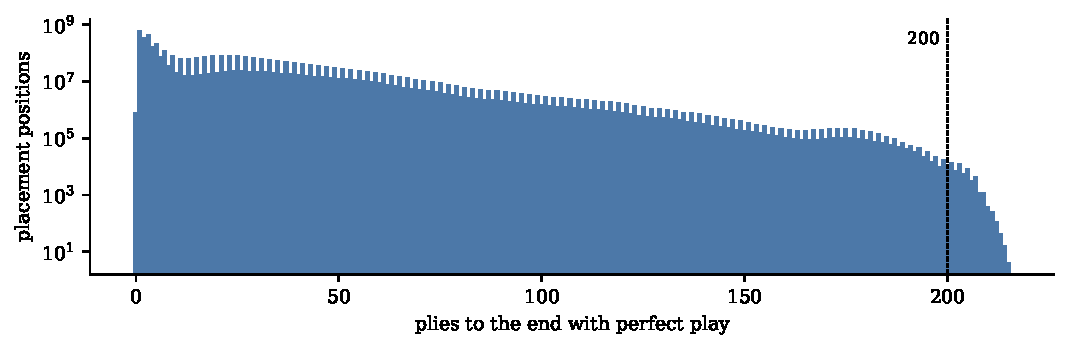
\includegraphics[width=0.95\linewidth]{figures/dtm_histogram.pdf}
\caption{Placement positions with a forced result, by plies to the end (logarithmic scale). Odd distances
are wins for the side to move and even ones losses. Half of these positions end within 9 plies. The count
falls roughly geometrically with the distance, has a shoulder between 160 and 190 plies, and stops at 215.}\label{fig:dtm}
\end{figure}

\section{The longest forced wins}\label{sec:longest}

How long can a won game last when both sides play perfectly, the winner as fast as possible and the loser as
slowly as possible? The tables answer this directly, but one more step is needed to get an answer about
real games.

\subsection{Over all positions: 215 plies, in positions no game reaches}

The largest distance in the tables is $\max_x d(x) = 215$. It occurs in four positions (two mirror pairs),
all with the goats to move after 4 or 5 goats are placed and none captured, for example tigers on
$\{4, 12, 13\}$ and goats on $\{3, 5, 6, 22\}$ (Figure~\ref{fig:records}, right). The goats win, and they have
exactly one winning move.

None of the four can occur in a game. This was noticed by looking at the board, and the argument is short.

\begin{lemma}\label{lem:unreachable}
Let $x$ be a placement position with no captures in which the tigers stand on $T$. Let $\Delta(T)$ be the
smallest total graph distance from the starting squares $\{0, 3, 4\}$ to $T$ over all ways of matching the
three tigers to the three squares. If $\Delta(T)$ exceeds the number of tiger moves made before $x$, then $x$
is unreachable.
\end{lemma}

\begin{proof}
With no capture, every tiger move so far was a slide along one edge, which changes the total distance
travelled by 1. Reaching $T$ needs at least $\Delta(T)$ slides.
\end{proof}

For $T = \{4, 12, 13\}$, $\Delta(T) = 7$. With 4 goats placed and the goats to move, the tigers have made 4
moves if the goats moved first and 5 if the tigers did. The other three positions fail in the same way
($\Delta = 7$ against at most 6 moves).

The tables hold every arrangement of pieces because the recursion needs no more than that, and a position's
value never depends on how it arose. Every stored value is therefore correct. But a maximum taken over all
arrangements is a statement about arrangements, not about games.

\subsection{Reachable positions}

\begin{definition}
For a first mover $f \in \{\gt, \tg\}$, let $x_0^f$ be the opening position (tigers on $\{0, 3, 4\}$, no goats,
$f$ to move). $\Reach_f$ is the smallest set that contains $x_0^f$ and, with every position, all its
successors. For $x \in \Reach_f$, $\delta_f(x)$ is the fewest plies in which a game from $x_0^f$ reaches $x$.
\end{definition}

$\Reach_f$ is computed by a forward search over the same layers and with the same move code as the solver
(\code{reachable.py}; Algorithm~\ref{alg:reach}).

\begin{algorithm}[H]
\caption{Reachable positions and their fewest plies, for first mover $f$}\label{alg:reach}
\begin{tabbing}
\hspace{1.6em}\=\hspace{1.6em}\=\hspace{1.6em}\=\kill
mark $x_0^f$ \\
\textbf{placement, forwards:} for the layers in the order $\Pi^{\tg}_0, \Pi^{\gt}_0, \Pi^{\tg}_1, \Pi^{\gt}_1, \dots, \Pi^{\gt}_{14}$: \\
\> for every marked position of the layer, mark all its successors \\
\textbf{movement, breadth-first:} the successors of $\Pi^{\gt}_{14}$ are the entry positions; set $\delta_f = t_0$ on them \\
\> \textbf{for} $j = t_0, t_0 + 1, \dots$ until nothing new is found: \\
\>\> for every position with $\delta_f = j$ and every successor $y$ without a value: $\delta_f(y) \leftarrow j + 1$
\end{tabbing}
\end{algorithm}

\begin{proposition}\label{prop:reach}
Algorithm~\ref{alg:reach} marks exactly $\Reach_f$, and its $\delta_f$ is the fewest plies from the opening.
In the placement phase the number of plies is the same along every route:
$\delta_f(x) = 2n$ (goats to move) or $2n - 1$ (tigers to move) for $f = \gt$, and $2n + 1$ or $2n$ for $f = \tg$.
\end{proposition}

\begin{proof}
Every placement move goes from a layer to a later one in the stated order (Section~\ref{sec:dp-graph}). When a
layer is processed, all its predecessors' layers are finished, so its marks are final; by induction along
the order the marked set is closed under successors and contains only positions with a marked predecessor
chain to $x_0^f$. The ply count is fixed because each goat turn places exactly one goat and the sides
alternate. In the movement phase every entry position has the same $\delta_f = t_0$ (29 for $f = \gt$, 30 for
$f = \tg$), and breadth-first search from a set of equal depth visits positions in order of distance, so the
first value written is the minimum. The search stops when a level adds nothing, at which point the marked
set is closed under successors.
\end{proof}

Table~\ref{tab:reach} gives the counts. Of the 19.02 billion positions, 18{,}189{,}005{,}282 are reachable when
the goats move first and 18{,}553{,}660{,}020 when the tigers do. Early layers are sparse: after three goats
only 153{,}510 of 2{,}392{,}621 goat-to-move positions can have arisen with the goats first. By the end of
the placement phase, every board with the tigers to move is reachable. The search needs only one more ply to
close: the positions first reached in the movement phase all appear at ply 30 ($f = \gt$) or 31
($f = \tg$). About 1\% of movement positions with the goats to move are never reached; these are boards on
which no tiger can have just moved.

\begin{table}[H]
\centering\scriptsize
\caption{Reachable positions by layer. ``All'' counts every arrangement, per side to move.}\label{tab:reach}
\begin{tabular}{@{}lr rr rr@{}}
\toprule
 & & \multicolumn{2}{c}{goats move first} & \multicolumn{2}{c}{tigers move first} \\
\cmidrule(lr){3-4}\cmidrule(l){5-6}
layer ($n$ placed) & all & goats to move & tigers to move & goats to move & tigers to move \\
\midrule
\tabin{generated/tab_reachable}
\bottomrule
\end{tabular}
\end{table}

\subsection{The longest forced wins of real games}

\begin{definition}
For a first mover $f$ and a winner $w \in \{\gt, \tg\}$,
\begin{align*}
\ell^*_f(w) &= \max\{\, d(x) : x \in \Reach_f,\ w \text{ wins at } x \,\}, \\
\ell^{200}_f(w) &= \max\{\, d(x) : x \in \Reach_f,\ w \text{ wins at } x,\ \delta_f(x) + d(x) \le 200 \,\}.
\end{align*}
\end{definition}

The second quantity is the longest forced win that the 200-ply limit of \code{TnGEnv} does not cut off. By
Proposition~\ref{prop:limit} a win from $x$ survives the limit exactly when the game reached $x$ early enough,
and the earliest it can do so is $\delta_f(x)$.

\begin{theorem}[Longest forced wins]\label{thm:longest}
\begin{center}
\begin{tabular}{@{}lcccc@{}}
\toprule
first mover $f$ & $\ell^*_f(\text{goats})$ & $\ell^{200}_f(\text{goats})$ & $\ell^*_f(\text{tigers})$ & $\ell^{200}_f(\text{tigers})$ \\
\midrule
goats & \textbf{213} & 191 & 67 & 67 \\
tigers & \textbf{214} & 193 & 67 & 67 \\
\bottomrule
\end{tabular}
\end{center}
\end{theorem}

\begin{proof}
The claim has three parts, and each is established by something checked exhaustively.

\emph{(i) The distances are exact.} $d(x)$ in the tables is the true distance for every position, by
Theorem~\ref{thm:certificate} and the full check of Section~\ref{sec:dp-proof}.

\emph{(ii) The set is exact.} The search marks exactly $\Reach_f$ with the true $\delta_f$, by
Proposition~\ref{prop:reach}. Its move generation is the solver's, which equals the environment's on every
board (Section~\ref{sec:dp-proof}).

\emph{(iii) The maximum is taken over all of it.} The program reads $d(x)$ for every marked position and
keeps the largest per winner, and the largest among those with $\delta_f(x) + d(x) \le 200$. Nothing is
sampled. This gives the upper bound: no reachable position has a longer forced win.

\emph{The bound is attained.} For each entry the program outputs a complete game. It walks back from the
record position $x^*$ through marked predecessors to $x_0^f$, which exhibits a legal route of length
$\delta_f(x^*)$, and then plays the perfect line from $x^*$. Each game has been replayed move by move with a
separate implementation of the rules: every move is legal, $x^*$ appears at ply $\delta_f(x^*)$, and the game
ends with the stated winner exactly $d(x^*)$ plies later (Appendix~\ref{app:games}).
\end{proof}

\begin{table}[H]
\centering\small
\caption{The record positions. ``Game'' is the length of the witness game: $\delta_f(x^*) + d(x^*)$.}\label{tab:records}
\begin{tabular}{@{}llp{0.36\linewidth}rrr@{}}
\toprule
$f$ & quantity & position $x^*$ & $\delta_f$ & $d$ & game \\
\midrule
goats & $\ell^*(\text{goats})$ & tigers 1, 5, 8; goats 0, 6, 15, 18, 22; goats to move & 10 & 213 & 223 \\
goats & $\ell^{200}(\text{goats})$ & tigers 4, 5, 8; goats 1, 2, 17; goats to move & 6 & 191 & 197 \\
goats & $\ell^*(\text{tigers})$ & tigers 1, 5, 13; goats 6, 7, 8, 10, 11, 12, 18; 3 captured; tigers to move & 19 & 67 & 86 \\
tigers & $\ell^*(\text{goats})$ & tigers 1, 6, 14; goats 10, 16, 18--22; tigers to move & 14 & 214 & 228 \\
tigers & $\ell^{200}(\text{goats})$ & tigers 0, 5, 7; goats 3, 4, 19; goats to move & 7 & 193 & 200 \\
tigers & $\ell^*(\text{tigers})$ & tigers 1, 5, 13; goats 6, 7, 8, 10, 11, 12, 18; 3 captured; tigers to move & 20 & 67 & 87 \\
\bottomrule
\end{tabular}
\end{table}

\begin{figure}[H]
\centering
\begin{tabular}{ccc}
\tngboard{1,5,8}{0,6,15,18,22}{0.78} & \tngboard{1,6,14}{10,16,18,19,20,21,22}{0.78} & \tngboard{4,12,13}{3,5,6,22}{0.78} \\
\footnotesize goats first: goats to move, & \footnotesize tigers first: tigers to move, & \footnotesize unreachable: goats to move, \\
\footnotesize goats win in 213 & \footnotesize goats win in 214 & \footnotesize goats win in 215
\end{tabular}
\caption{The two record positions of real games, and one of the four positions with the largest distance
over all arrangements. Filled circles are tigers, open circles goats.}\label{fig:records}
\end{figure}

\paragraph{Reading the result.}
\begin{itemize}
\item The reachable records are only one and two plies short of the figure over all arrangements. The
  unreachable positions were not outliers; they sit at the end of a family of very long goat wins.
\item Both records are goat wins that begin early in the placement phase and end with the tigers
  immobilized. The goats' task is slow: they must place eleven or ten more goats and then close the net.
\item The tigers' wins are much shorter. A tiger win is a sequence of captures, and the longest one a game
  can reach takes 67 plies from a position in which three goats are already gone.
\item Both record wins end after ply 200 (at plies 223 and 228 by the shortest route). Under the limit of
  \code{TnGEnv} they would be cut off as draws. The longest win that fits takes 191 plies (goats first) or
  193 (tigers first, ending exactly at ply 200).
\item In the movement phase the largest distance is 210 plies (tigers to move, 15 goats, no captures). That
  position is reachable, but only from ply 29, so its game would last at least 239 plies.
\end{itemize}

\paragraph{Independent checks of this section.} A separate search written in plain Python, sharing no code
with the GPU search, reproduces the reachable counts exactly for the layers with up to four goats placed, for
both first movers (20 layer counts, from 1 to 3{,}295{,}989 positions). All six witness games were replayed
with the visualizer's rule implementation, which is itself tested against \code{TnGEnv}.


\part{Comparisons}
\section{Evaluation protocol and metrics}\label{old:7}

\textbf{Games.}

\begin{itemize}
\item Game $i \in \{0, \dots, G-1\}$ resets every random generator and the environment with seed $s_0 + i$ ($s_0 = 10{,}000$ in the study, \code{EVAL\_\allowbreak{}SEED} in the notebooks), so every model faces the same games.
\item The learner plays deterministically (\S\ref{old:3.2}).
\item The opponent is a fixed tiger, greedy or smart, with no mixing.
\item The study uses $G = 1000$ per cell for final models and $G = 200$ per checkpoint.
\end{itemize}
\textbf{Play modes.}

{\small
\begin{longtable}{@{}lll@{}}
\toprule
\textbf{Mode} & \textbf{Learner action} & \textbf{Illegal move} \\
\midrule
\endhead
masked & $\arg\max_{a \in \mathcal{L}(s)} z_a$ & impossible \\
raw & $\arg\max_{a \in \mathcal{A}} z_a$ & ends the game (IllegalMove) \\
raw, lose a turn & $\arg\max_{a \in \mathcal{A}} z_a$ & costs a turn (\S\ref{old:2.3}) \\
\bottomrule
\end{longtable}\addtocounter{table}{-1}
}

Raw play is deterministic and an illegal attempt leaves $s$ unchanged. In lose-a-turn mode, a model that picks an illegal action therefore repeats it until the turn limit.

\textbf{Metrics.}

{\footnotesize
\begin{longtable}{@{}>{\raggedright\arraybackslash}p{\dimexpr 0.348\linewidth-2\tabcolsep\relax}>{\raggedright\arraybackslash}p{\dimexpr 0.652\linewidth-2\tabcolsep\relax}@{}}
\toprule
\textbf{Metric} & \textbf{Definition} \\
\midrule
\endhead
win rate $W$ & $\#\{\text{Goat wins}\}/G$; standard error $\sqrt{W(1-W)/G} \leq 1.6$ pp at $G = 1000$, $\leq 3.5$ pp at $G = 200$ \\
illegal endings & fraction of raw games ended by an illegal move \\
illegal probability by phase & $\bar P^{\text{ill}}_{\varphi} = \operatorname{mean}\{1 - P_{\mathcal{L}}(s) : s \text{ visited in masked play},\ \phi(s) = \varphi\}$, for $\varphi \in \{0, 1\}$ \\
\code{train/illegal\_\allowbreak{}prob} (TensorBoard) & $\mathbb{E}_{\mathcal{B}}[1 - P_{\mathcal{L}}(s_t)]$ averaged over a rollout's minibatches: on-policy, training states \\
window win rate (TensorBoard) & goat wins over the last 1,000 training episodes. These use sampled actions and the $q = 0.5$ mix, so they are not comparable to $W$ \\
\bottomrule
\end{longtable}\addtocounter{table}{-1}
}


\section{The legality study}\label{old:9}

\textbf{Question.} Can a policy trained \emph{without} the mask learn the rules well enough to play legally on its own? Does that cost or gain playing strength compared with Maskable PPO, and which objective (\S\ref{old:5}) gets there? Setup: \S\ref{old:6.4}. Protocol: \S\ref{old:7}.

\textbf{Which rules.} Every number in this section was measured in \code{TnGEnv} before the capture correction of Section~\ref{sec:rulefix}, the rule under which all these models were trained. Section~\ref{sec:cmp-fix} repeats the comparison under the corrected rule; the conclusions about legality do not depend on it.

\subsection{Final models, tanh (1,000 games per cell)}\label{old:9.1}

$W$ is the goat win rate against each tiger. $\bar P^{\text{ill}}_0, \bar P^{\text{ill}}_1$ are the illegal probabilities in the placement and movement phases (\S\ref{old:7}).

{\footnotesize
\begin{longtable}{@{}>{\raggedright\arraybackslash}p{\dimexpr 0.275\linewidth-2\tabcolsep\relax}>{\raggedleft\arraybackslash}p{\dimexpr 0.122\linewidth-2\tabcolsep\relax}>{\raggedleft\arraybackslash}p{\dimexpr 0.115\linewidth-2\tabcolsep\relax}>{\raggedleft\arraybackslash}p{\dimexpr 0.099\linewidth-2\tabcolsep\relax}>{\raggedleft\arraybackslash}p{\dimexpr 0.092\linewidth-2\tabcolsep\relax}>{\raggedleft\arraybackslash}p{\dimexpr 0.053\linewidth-2\tabcolsep\relax}>{\raggedleft\arraybackslash}p{\dimexpr 0.053\linewidth-2\tabcolsep\relax}>{\raggedleft\arraybackslash}p{\dimexpr 0.191\linewidth-2\tabcolsep\relax}@{}}
\toprule
\textbf{Model} & \textbf{$W$ masked, greedy} & \textbf{$W$ masked, smart} & \textbf{$W$ raw, greedy} & \textbf{$W$ raw, smart} & \textbf{$\bar P^{\text{ill}}_0$} & \textbf{$\bar P^{\text{ill}}_1$} & \textbf{Raw games ended illegally} \\
\midrule
\endhead
Maskable PPO, seed 42 & 0.692 & 0.599 & 0 & 0 & 0.778 & 0.876 & 100\% \\
Maskable PPO, seed 7 & 0.718 & 0.619 & 0 & 0 & 0.790 & 0.805 & 100\% \\
PPO, no legality loss, seed 42 & 0.530 & 0 & 0.525 & 0 & 0.549 & 0.881 & 73.8\% \\
PPO, no legality loss, seed 7 & 0.637 & 0 & 0.576 & 0 & 0.448 & 0.870 & 71.2\% \\
\textbf{PPO + nll 0.5, seed 42} & \textbf{0.754} & \textbf{0.947} & \textbf{0.752} & \textbf{0.947} & 0.0010 & 0.029 & 3.6\% \\
PPO + nll 0.5, seed 7 & 0.547 & 0.023 & 0.536 & 0.023 & 0.0034 & 0.062 & 23.4\% \\
PPO + nll 2, seed 42 & 0.714 & 0.795 & 0.714 & 0.795 & \textbf{0.0002} & \textbf{0.0015} & \textbf{0.1\%} \\
PPO + mass 0.5 & 0.006 & 0 & 0.006 & 0 & 0.0007 & 0.504 & 99.6\% \\
KL penalty + nll 0.5 & 0.566 & 0.445 & 0.564 & 0.445 & 0.0030 & 0.069 & 7.6\% \\
SPO + nll 0.5 & 0.005 & 0 & 0.005 & 0 & 0.0023 & 0.179 & 97.4\% \\
clip + nll 0.5 + Huber & 0.628 & 0.336 & 0.627 & 0.336 & 0.0015 & 0.018 & 1.5\% \\
\emph{shipped NormalGoat (100M, greedy)} & 0.796 & 0.016 & 0 & 0 & 0.977 & 0.973 & 100\% \\
\emph{shipped SmartGoat (100M, smart)} & 0.067 & 0.944 & 0 & 0 & 0.844 & 0.992 & 100\% \\
\emph{shipped RobustGoat (60M, curriculum)} & 0.798 & 0.857 & 0 & 0 & 0.984 & 0.990 & 100\% \\
\bottomrule
\end{longtable}\addtocounter{table}{-1}
}

The raw lose-a-turn win rates equal the raw win rates to three decimals for every model, so the table omits them.

\subsection{Training dynamics (TensorBoard, last \textasciitilde{}40k steps of each run)}\label{old:9.2}

{\small
\begin{longtable}{@{}>{\raggedright\arraybackslash}p{\dimexpr 0.231\linewidth-2\tabcolsep\relax}>{\raggedleft\arraybackslash}p{\dimexpr 0.167\linewidth-2\tabcolsep\relax}>{\raggedleft\arraybackslash}p{\dimexpr 0.222\linewidth-2\tabcolsep\relax}>{\raggedleft\arraybackslash}p{\dimexpr 0.157\linewidth-2\tabcolsep\relax}>{\raggedleft\arraybackslash}p{\dimexpr 0.222\linewidth-2\tabcolsep\relax}@{}}
\toprule
\textbf{Run} & \textbf{\code{train/illegal\_\allowbreak{}prob}} & \textbf{Illegal endings (window)} & \textbf{Win rate (window)} & \textbf{Win rate first ≥ 0.10 at} \\
\midrule
\endhead
Maskable PPO (42 / 7) & — & 0 / 0 & 0.567 / 0.594 & 0.49M / 0.57M \\
no legality loss (42 / 7) & 0.119 / 0.114 & 0.756 / 0.750 & 0.244 / 0.250 & 1.39M / 1.72M \\
nll 0.5 (42 / 7) & 0.004 / 0.020 & 0.084 / 0.440 & 0.798 / 0.152 & 5.00M / 9.26M \\
nll 2 & 0.000 & 0.005 & 0.680 & 3.77M \\
mass 0.5 & 0.049 & 0.999 & 0.001 & never \\
KL penalty + nll 0.5 & 0.022 & 0.489 & 0.163 & 9.34M \\
SPO + nll 0.5 & 0.042 & 0.877 & 0.000 & never \\
clip + nll 0.5 + Huber & 0.006 & 0.119 & 0.324 & 5.98M \\
\bottomrule
\end{longtable}\addtocounter{table}{-1}
}


\begin{figure}[H]
\centering
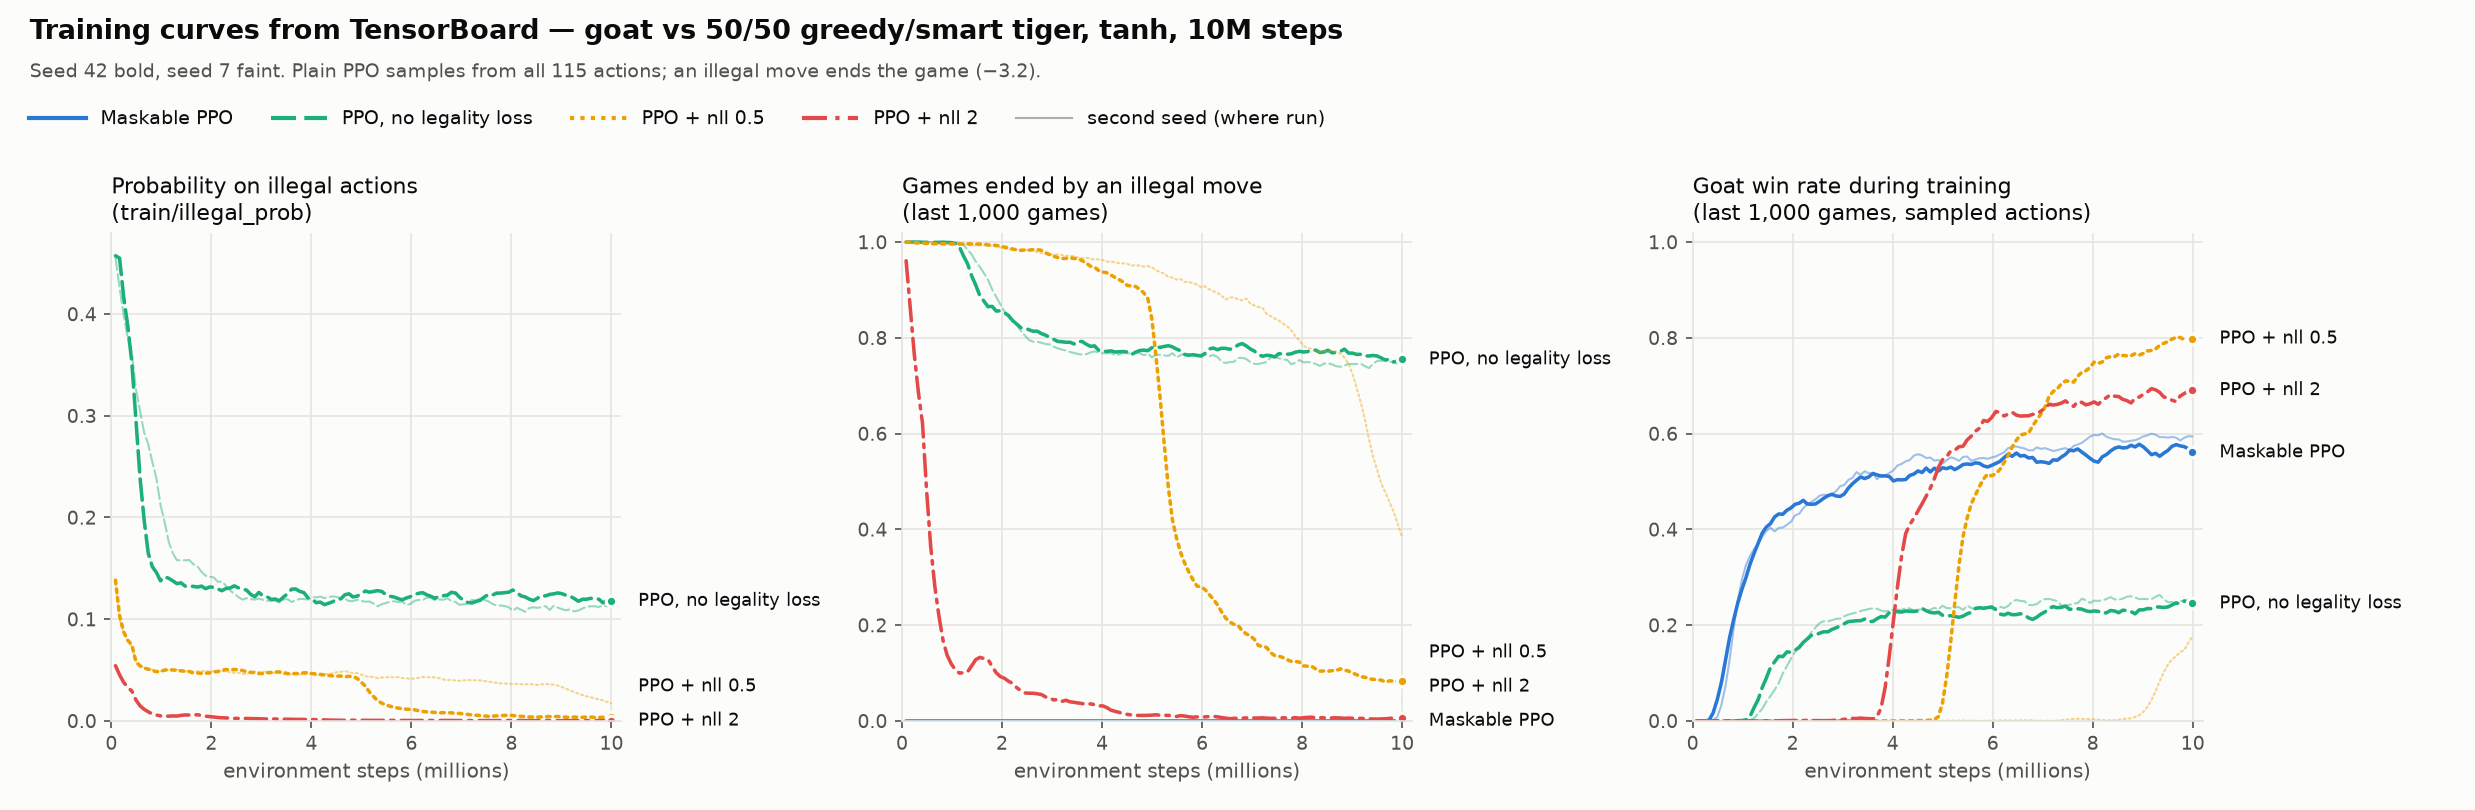
\includegraphics[width=0.98\linewidth]{figures/1_training_curves.png}
\caption{Training curves of the tanh runs of the legality study (TensorBoard).}\label{fig:curves}
\end{figure}

\begin{figure}[H]
\centering
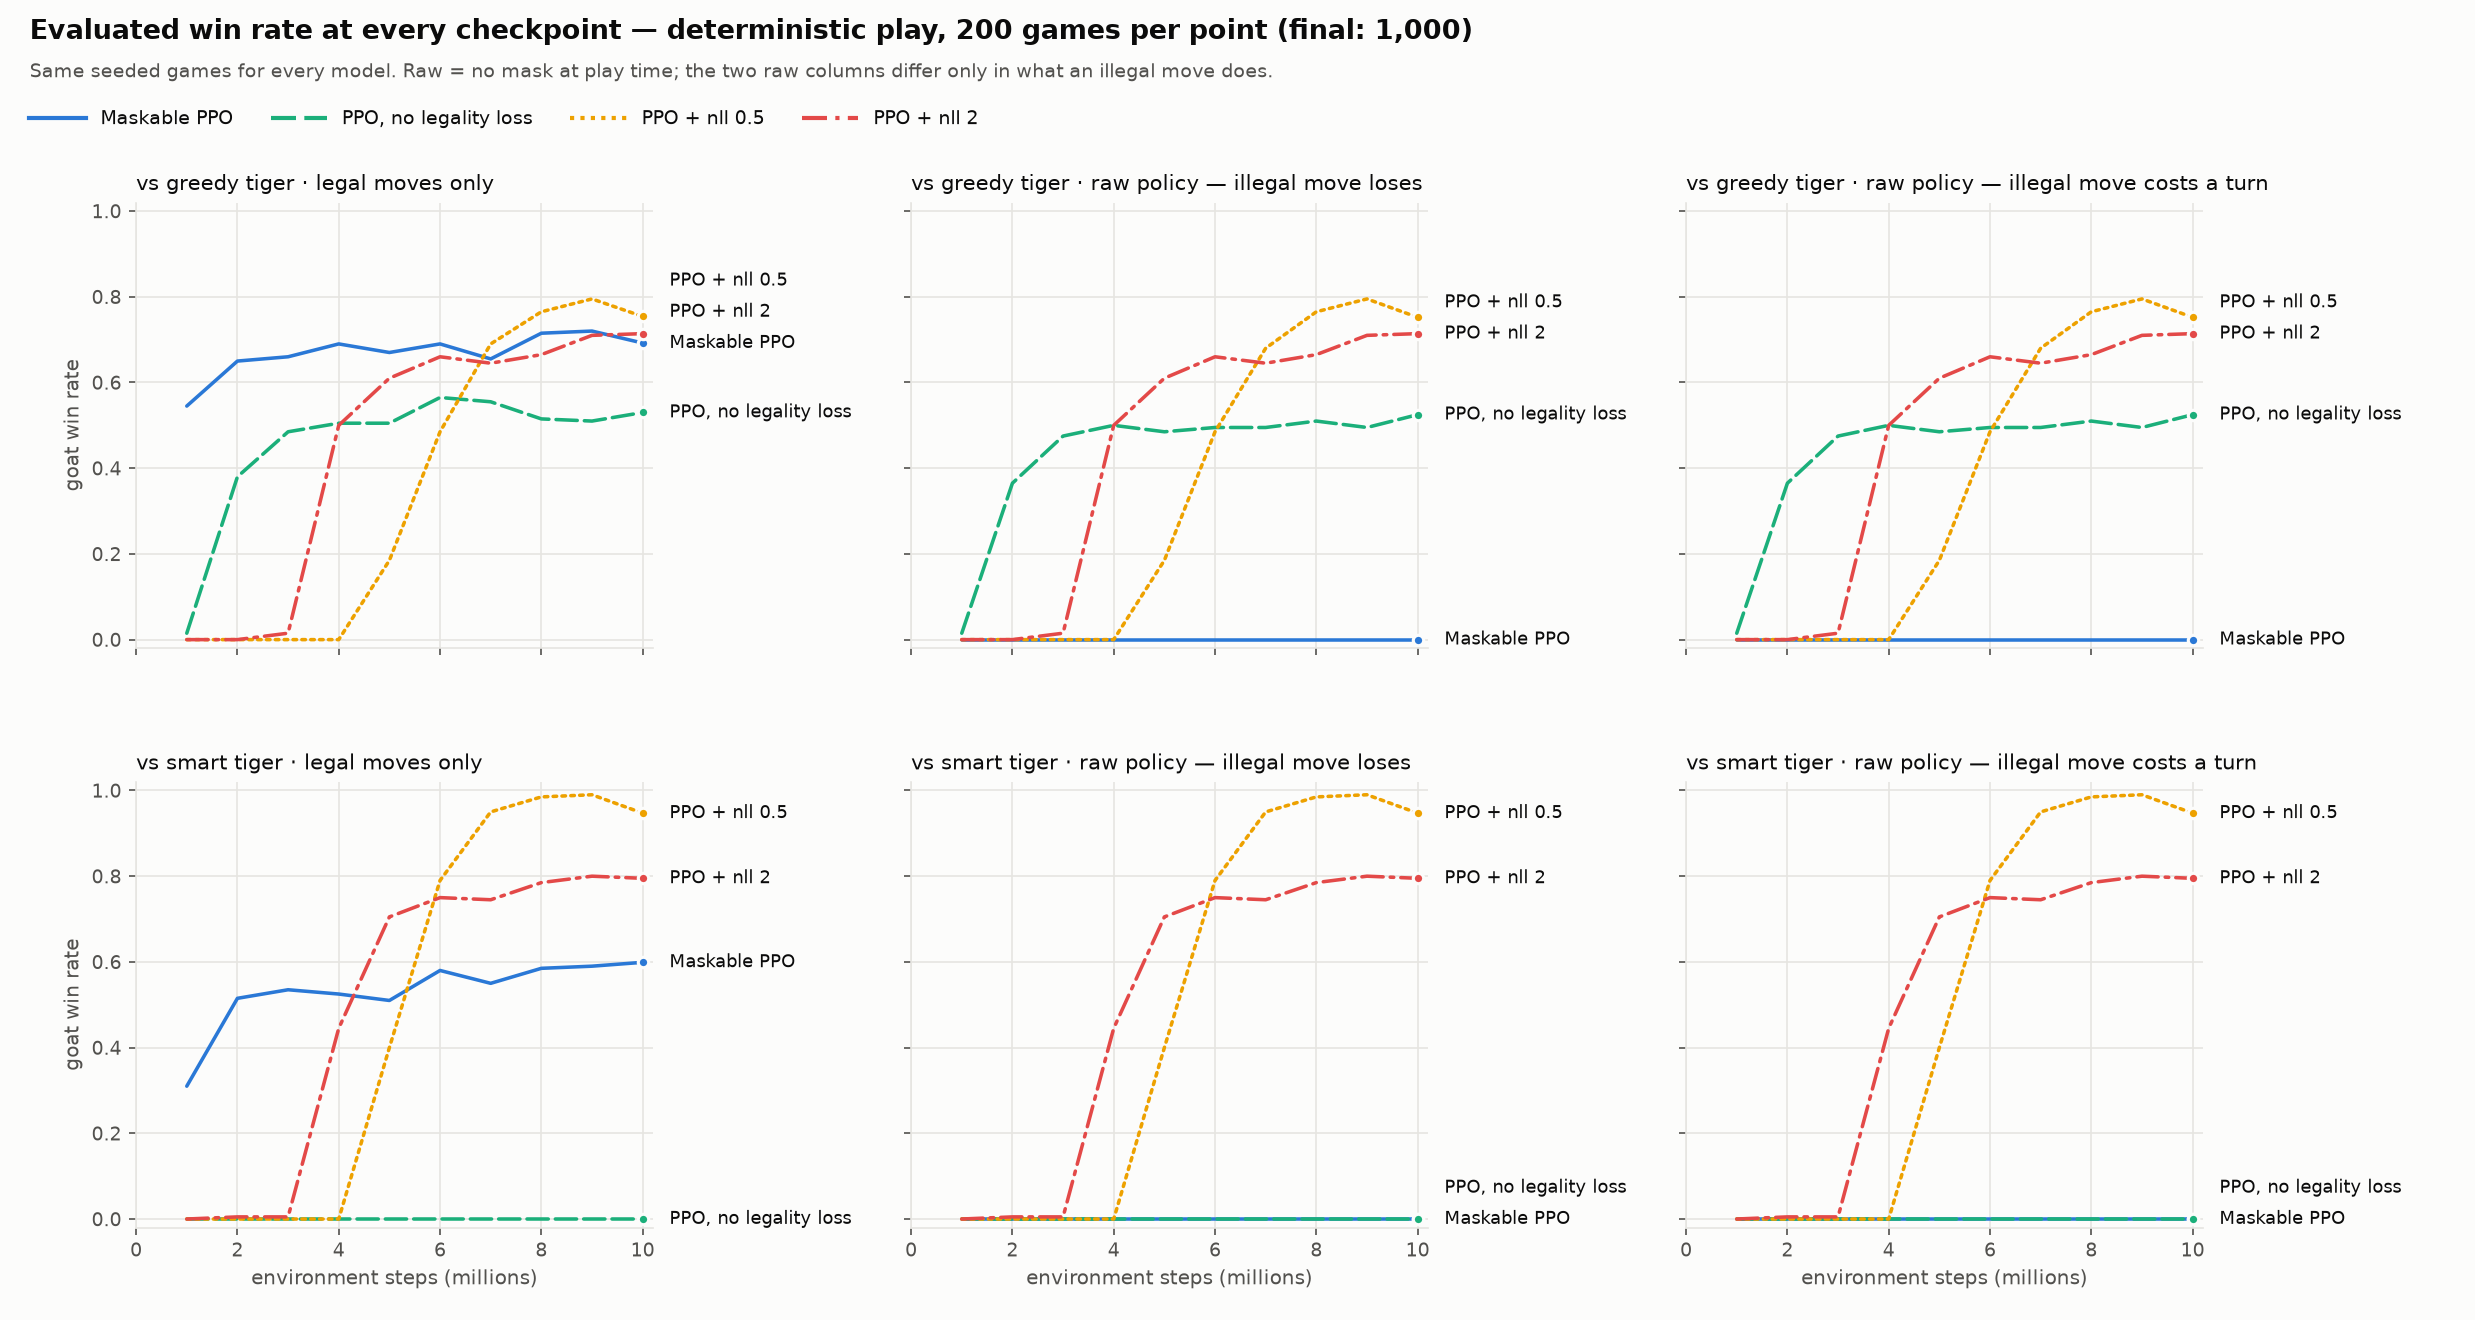
\includegraphics[width=0.98\linewidth]{figures/2_checkpoint_eval.png}
\caption{Checkpoint evaluations every 1M steps (200 games per point).}\label{fig:ckpt}
\end{figure}

\subsection{Findings}\label{old:9.3}

\begin{enumerate}
\item \textbf{Masking teaches the network nothing about legality.} After 10M steps, Maskable PPO still puts 78–88\% of its raw probability on illegal actions. The shipped models put 84–99\% there after 60–100M steps. Without the mask they lose every game. This is the zero-gradient property of \S\ref{old:3.2}: no loss term ever touches an illegal logit.
\item \textbf{The reward alone teaches legality only partly.} Plain PPO with $c_{\text{legal}} = 0$ learns to avoid most illegal moves in deterministic play (53–58\% raw wins against greedy). But it keeps 11–12\% illegal probability on its training states, and 71–74\% of its raw games still end in an illegal move. It never beats the smart tiger.
\item \textbf{The \code{nll} legality loss gives fully legal play and, for seed 42, the strongest goat in the study.} With $c_{\text{legal}} = 0.5$ (seed 42), masked and raw win rates agree to 0.002. Of its 3.6\% illegal raw endings, at most 2 in 2,000 games are games it wins with the mask. Against the smart tiger it wins 94.7\%, against 59.9\% for Maskable PPO at the same budget and 85.7\% for the 60M-step RobustGoat. With $c_{\text{legal}} = 2$ the network is almost perfectly legal ($\bar P^{\text{ill}}_1 = 0.0015$) and still strong (71.4\% / 79.5\%).
\item \textbf{Training under ``end\_game'' has a long plateau, then a sharp take-off.} An illegal move ends the episode, so a winning game needs every move to be legal. With per-move illegal probability $p$, the chance of playing $n$ moves without one is $(1-p)^n$. At $p \approx 0.05$ and $n \approx 25$ moves, that is about 0.28, and the agent almost never reaches the movement phase. The \code{nll} term pushes $p$ down until play survives long enough for winning rewards to appear. The take-off then comes at 3.8M ($c_{\text{legal}} = 2$), 5.0M or 9.3M (two seeds of 0.5). The onset time is very seed-sensitive, which is why seed 7 of \code{nll} 0.5 ends far behind seed 42.
\item \textbf{\code{mass} fails, as \S\ref{old:5.4} predicts.} Its gradient on an illegal logit is $\pi(a \mid s)\,P_{\mathcal{L}}(s)$, which is tiny while $P_{\mathcal{L}}$ is tiny. It cleans up the placement phase ($\bar P^{\text{ill}}_0 = 0.0007$) but leaves half the movement-phase probability illegal, and 99.6\% of games end illegally.
\item \textbf{The policy loss matters.} With the same legality term, SPO never took off and KL penalty took off only at 9.3M. Huber took off at 6M and finished weaker than plain MSE. These are single seeds, and finding 4 shows how much the onset time varies between seeds. So these rank orders are suggestive, not established.
\end{enumerate}
\textbf{Limitations.}

\begin{itemize}
\item Most variants have one seed.
\item Evaluation uses the training opponents (greedy and smart).
\item The shipped models were trained on an earlier environment version (\S\ref{old:6.2}).
\item Win rate is measured with deterministic play only.
\end{itemize}
\subsection{ReLU vs tanh}\label{old:9.4}

Same settings and seed as \S\ref{old:9.1}, with $\operatorname{act} = $ ReLU (\S\ref{old:3.1}). 1,000 games per cell (Figure~\ref{fig:relu}).

{\footnotesize
\begin{longtable}{@{}>{\raggedright\arraybackslash}p{\dimexpr 0.382\linewidth-2\tabcolsep\relax}>{\raggedright\arraybackslash}p{\dimexpr 0.049\linewidth-2\tabcolsep\relax}>{\raggedleft\arraybackslash}p{\dimexpr 0.130\linewidth-2\tabcolsep\relax}>{\raggedleft\arraybackslash}p{\dimexpr 0.122\linewidth-2\tabcolsep\relax}>{\raggedleft\arraybackslash}p{\dimexpr 0.106\linewidth-2\tabcolsep\relax}>{\raggedleft\arraybackslash}p{\dimexpr 0.098\linewidth-2\tabcolsep\relax}>{\raggedleft\arraybackslash}p{\dimexpr 0.057\linewidth-2\tabcolsep\relax}>{\raggedleft\arraybackslash}p{\dimexpr 0.057\linewidth-2\tabcolsep\relax}@{}}
\toprule
\textbf{Model} & \textbf{act} & \textbf{$W$ masked, greedy} & \textbf{$W$ masked, smart} & \textbf{$W$ raw, greedy} & \textbf{$W$ raw, smart} & \textbf{$\bar P^{\text{ill}}_0$} & \textbf{$\bar P^{\text{ill}}_1$} \\
\midrule
\endhead
Maskable PPO & tanh & 0.692 & 0.599 & 0 & 0 & 0.778 & 0.876 \\
Maskable PPO & ReLU & \textbf{0.854} & \textbf{0.856} & 0 & 0 & 0.924 & 0.887 \\
PPO, no legality loss & tanh & 0.530 & 0 & 0.525 & 0 & 0.549 & 0.881 \\
PPO, no legality loss & ReLU & 0.008 & 0 & 0.002 & 0 & 0.010 & 0.843 \\
PPO + nll 0.5 & tanh & 0.754 & 0.947 & 0.752 & 0.947 & 0.0010 & 0.029 \\
PPO + nll 0.5 & ReLU & 0.662 & 0.743 & 0.660 & 0.743 & 0.0010 & 0.0084 \\
PPO + nll 2 & tanh & 0.714 & 0.795 & 0.714 & 0.795 & 0.0002 & 0.0015 \\
PPO + nll 2 & ReLU & 0.694 & 0.851 & 0.692 & 0.851 & 0.0001 & 0.0010 \\
KL penalty + nll 0.5 & tanh & 0.566 & 0.445 & 0.564 & 0.445 & 0.0030 & 0.069 \\
KL penalty + nll 0.5 & ReLU & 0.592 & 0 & 0.588 & 0 & 0.0035 & 0.066 \\
SPO + nll 0.5 & tanh & 0.005 & 0 & 0.005 & 0 & 0.0023 & 0.179 \\
SPO + nll 0.5 & ReLU & 0.009 & 0 & 0.009 & 0 & 0.0044 & 0.169 \\
PPO, no legality loss, lose a turn ($r_{\text{ill}} = -1$) & ReLU & 0.186 & 0.906 & 0.185 & 0.906 & 0.019 & 0.070 \\
PPO + nll 2, lose a turn ($r_{\text{ill}} = -1$) & ReLU & 0.011 & 0 & 0.011 & 0 & 0.0003 & 0.0026 \\
\bottomrule
\end{longtable}\addtocounter{table}{-1}
}

Findings (one seed per cell, so differences within about the seed spread of \S\ref{old:9.1} are not significant):

\begin{enumerate}
\item ReLU helps Maskable PPO the most: it becomes the strongest player under the mask (0.854 / 0.856), but it still needs the mask ($\bar P^{\text{ill}} \approx 0.9$).
\item With the \code{nll} loss, the ReLU and tanh results fall inside the seed-to-seed spread of tanh \code{nll} 0.5 (0.547–0.754 vs greedy, 0.023–0.947 vs smart). \code{nll} 2 is the most consistent across activations (0.69–0.71 vs greedy, 0.80–0.85 vs smart), with almost no illegal probability.
\item Without a legality loss, ReLU with ``end\_game'' handling never learned to win. With ``lose a turn'', the same learner reached 0.906 against the smart tiger but only 0.186 against greedy. \code{nll} 2 with ``lose a turn'' failed to win at all, although it plays legally. Under ``lose a turn'' an illegal attempt does not end the game, so the pressure to be legal comes only from the $-1$ reward and the legality loss.
\end{enumerate}

\begin{figure}[H]
\centering
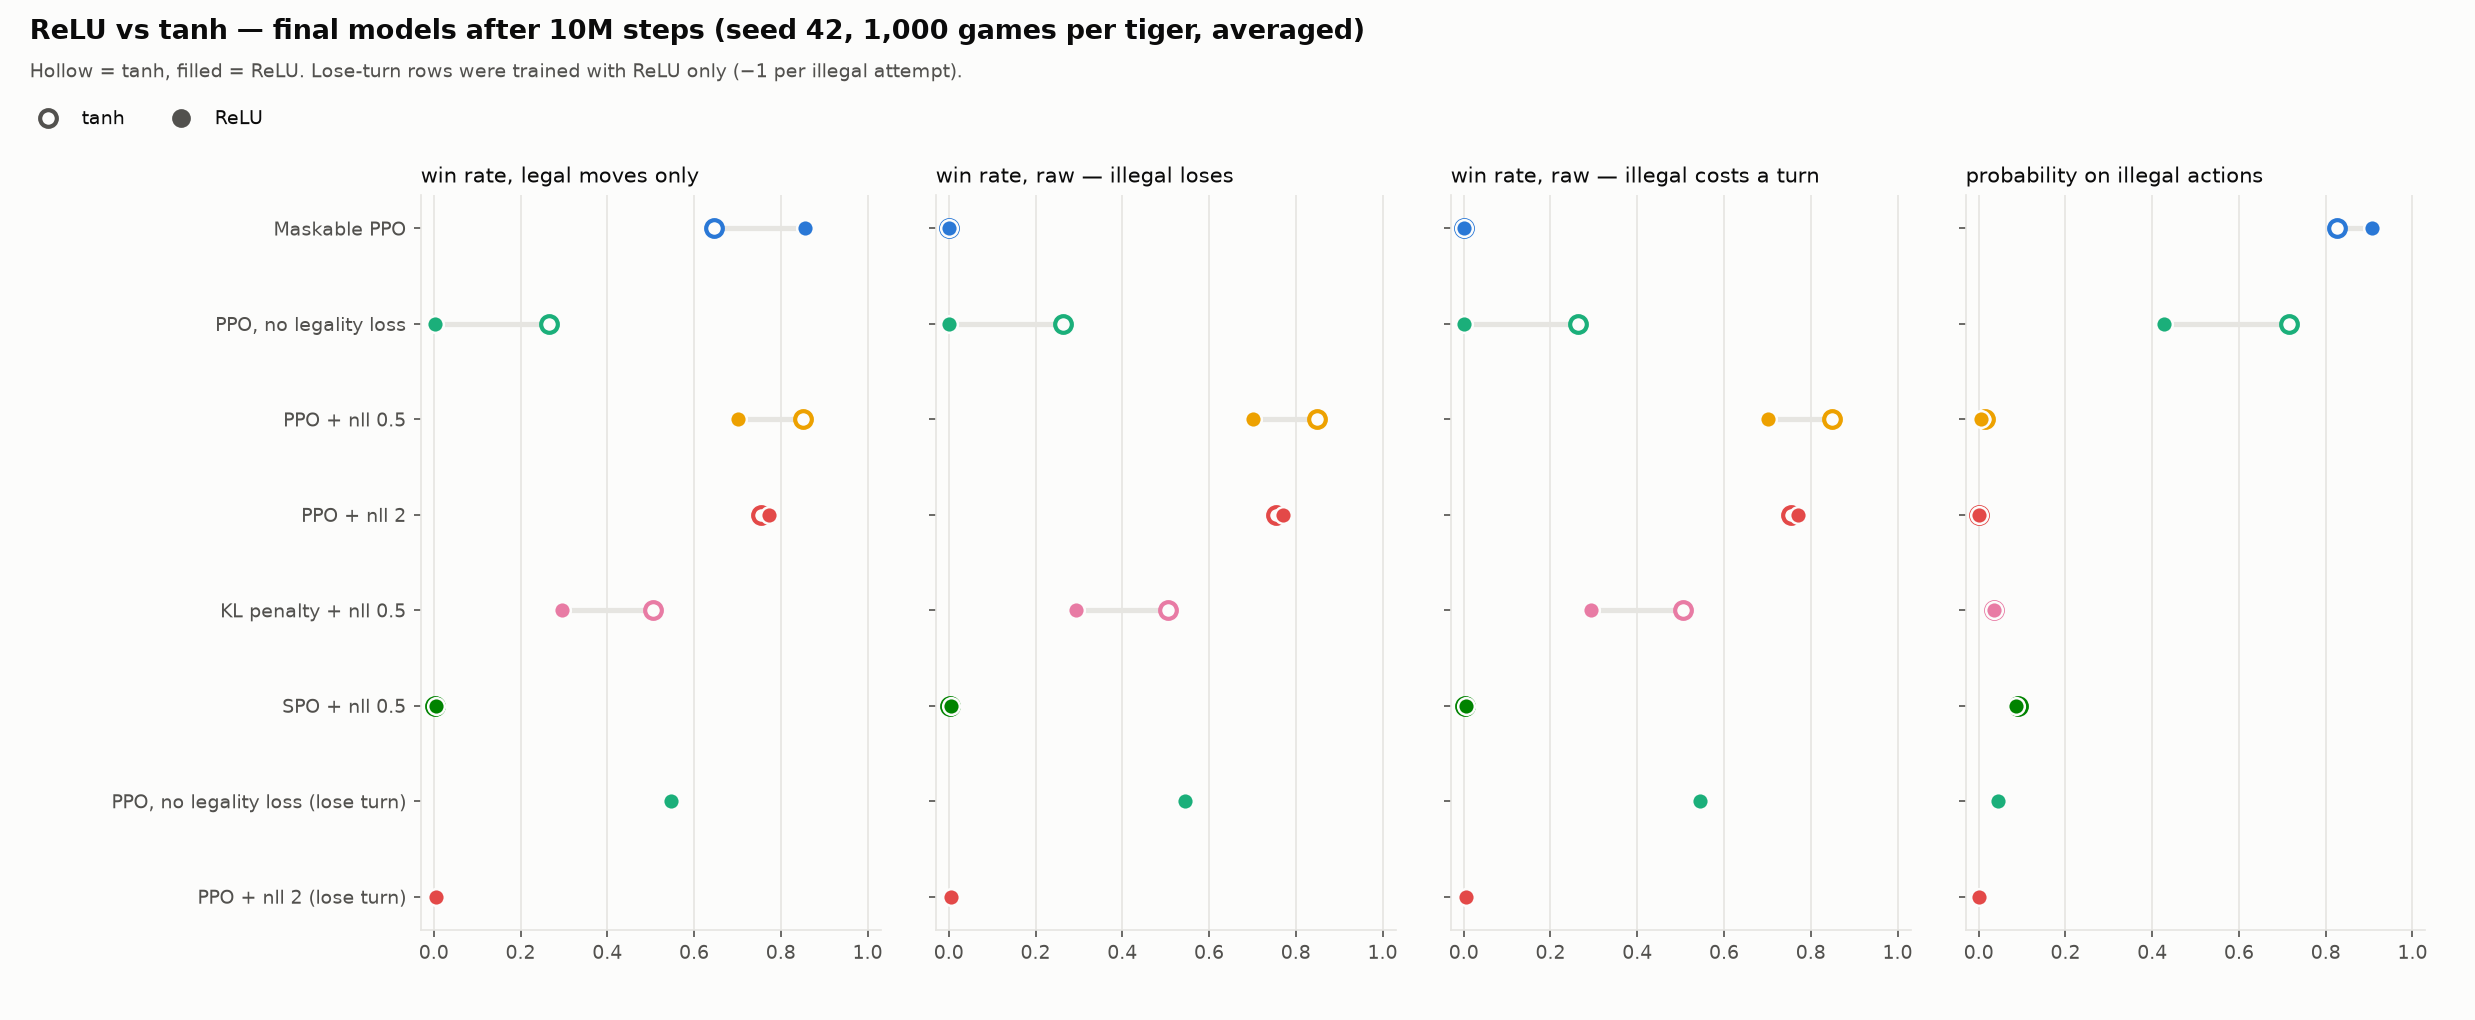
\includegraphics[width=0.8\linewidth]{figures/4_relu_vs_tanh.png}
\caption{ReLU against tanh, final models.}\label{fig:relu}
\end{figure}

\subsection{Variance of the invalid-action probability for the best model}\label{old:9.5}

Model: PPO + nll 0.5, tanh, seed 42. It played the 2,000 games of \S\ref{old:7} (1,000 per tiger) on its own: raw, argmax, an illegal move ends the game. At every decision we record $p_t = 1 - P_{\mathcal{L}}(s_t)$. Both sides are summed directly from float64 log-probabilities, so values down to about $10^{-9}$ are exact.

{\footnotesize
\begin{longtable}{@{}lrrrrrrrr@{}}
\toprule
\textbf{Decisions} & \textbf{$n$} & \textbf{mean $\bar p$} & \textbf{variance $\operatorname{Var}(p)$} & \textbf{std} & \textbf{median} & \textbf{95th pct} & \textbf{99th pct} & \textbf{max} \\
\midrule
\endhead
all & 46,810 & $4.23\times10^{-3}$ & $1.14\times10^{-3}$ & 0.034 & $4.0\times10^{-5}$ & $8.3\times10^{-3}$ & 0.094 & 0.995 \\
placement phase & 29,873 & $9.9\times10^{-4}$ & $1.27\times10^{-4}$ & 0.011 & $2.9\times10^{-5}$ & $2.5\times10^{-3}$ & 0.015 & 0.966 \\
movement phase & 16,937 & $9.95\times10^{-3}$ & $2.87\times10^{-3}$ & 0.054 & $7.6\times10^{-5}$ & 0.036 & 0.261 & 0.995 \\
vs greedy & 18,328 & $9.56\times10^{-3}$ & $2.79\times10^{-3}$ & 0.053 & $5.9\times10^{-5}$ & 0.031 & 0.254 & 0.995 \\
vs greedy, movement & 3,455 & 0.044 & 0.0123 & 0.111 & $4.4\times10^{-3}$ & 0.254 & 0.613 & 0.995 \\
vs smart & 28,482 & $8.05\times10^{-4}$ & $4.30\times10^{-5}$ & 0.0066 & $3.8\times10^{-5}$ & $2.2\times10^{-3}$ & 0.012 & 0.641 \\
\bottomrule
\end{longtable}\addtocounter{table}{-1}
}

\textbf{Decomposition.} By the law of total variance over games $j$:

\[
\operatorname{Var}(p) = \underbrace{\mathbb{E}_j\big[\operatorname{Var}(p \mid j)\big]}_{9.94\times10^{-4}\ (87\%)} + \underbrace{\operatorname{Var}_j\big(\mathbb{E}[p \mid j]\big)}_{1.44\times10^{-4}\ (13\%)}
\]
Most of the spread is between moves \emph{within} a game rather than between games.

\textbf{What drives it.} The distribution is heavy-tailed: half the decisions have $p_t < 4\times10^{-5}$, but rare movement-phase positions against the greedy tiger reach $p_t > 0.25$. The illegal probability rises through the game against greedy, from about $10^{-5}$ in early placement to a median near $2\times10^{-2}$ late in the movement phase. Against smart it stays near $10^{-4}$. In deterministic play only 73 of 46,810 choices were illegal.

\textbf{If the policy sampled instead of taking the argmax}, the probability that a whole game contains no illegal move along the same positions is $\prod_t (1 - p_t)$. Its mean is 0.93 (0.88 vs greedy, 0.98 vs smart).

\begin{figure}[H]
\centering
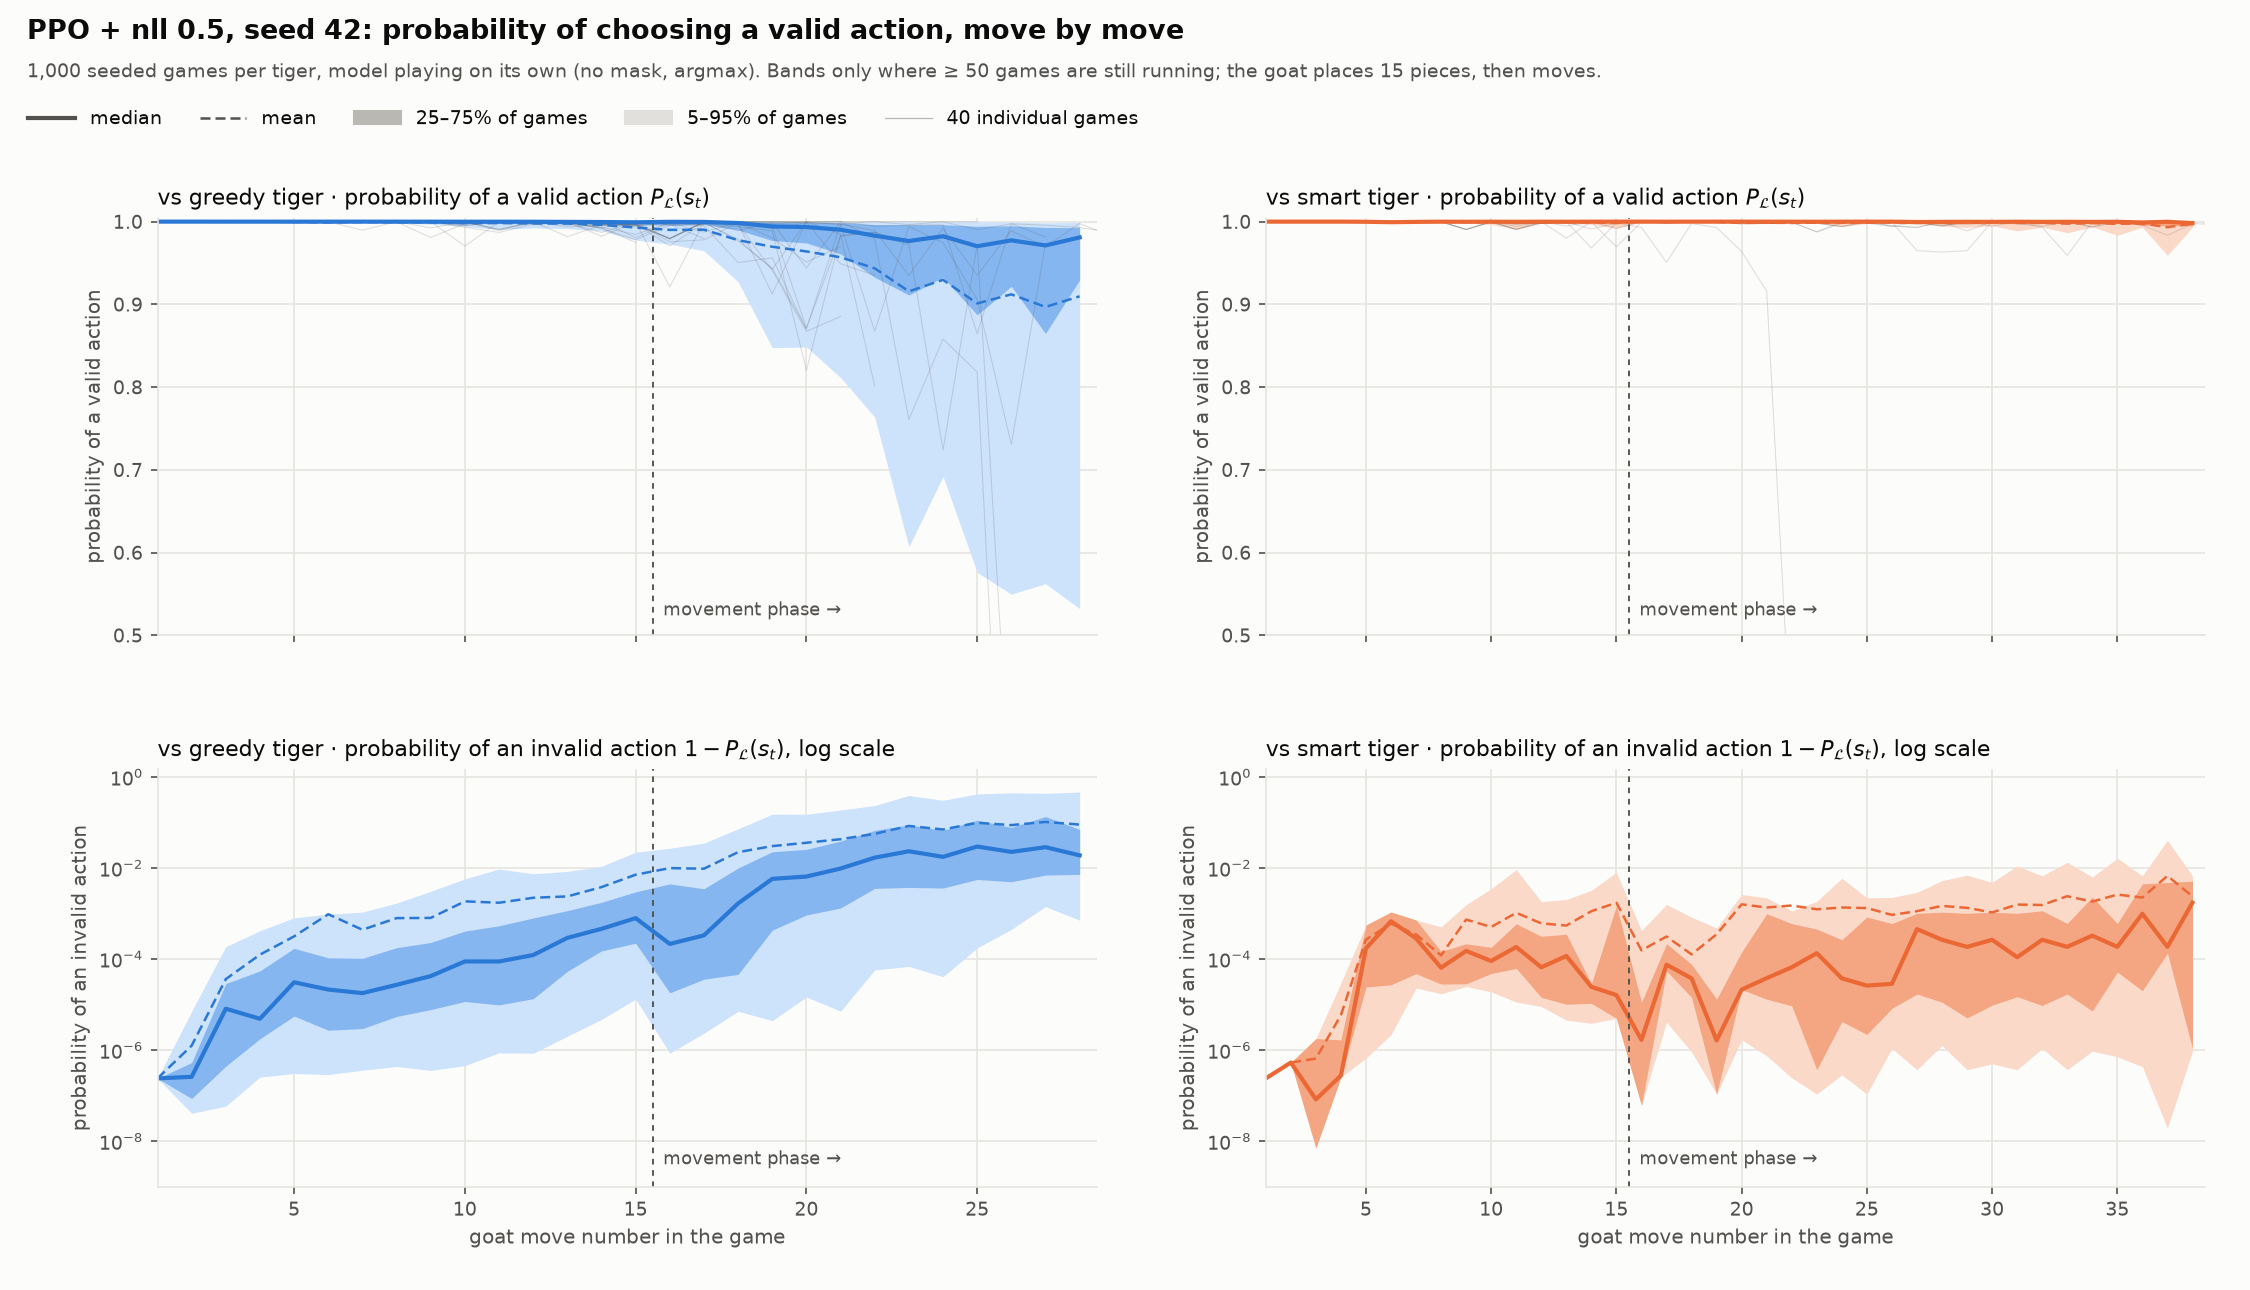
\includegraphics[width=0.98\linewidth]{figures/5_valid_probability_by_move.png}
\caption{Probability of a legal move by move number for the best model (PPO + nll 0.5, seed 42).}\label{fig:validprob}
\end{figure}

\begin{figure}[H]
\centering
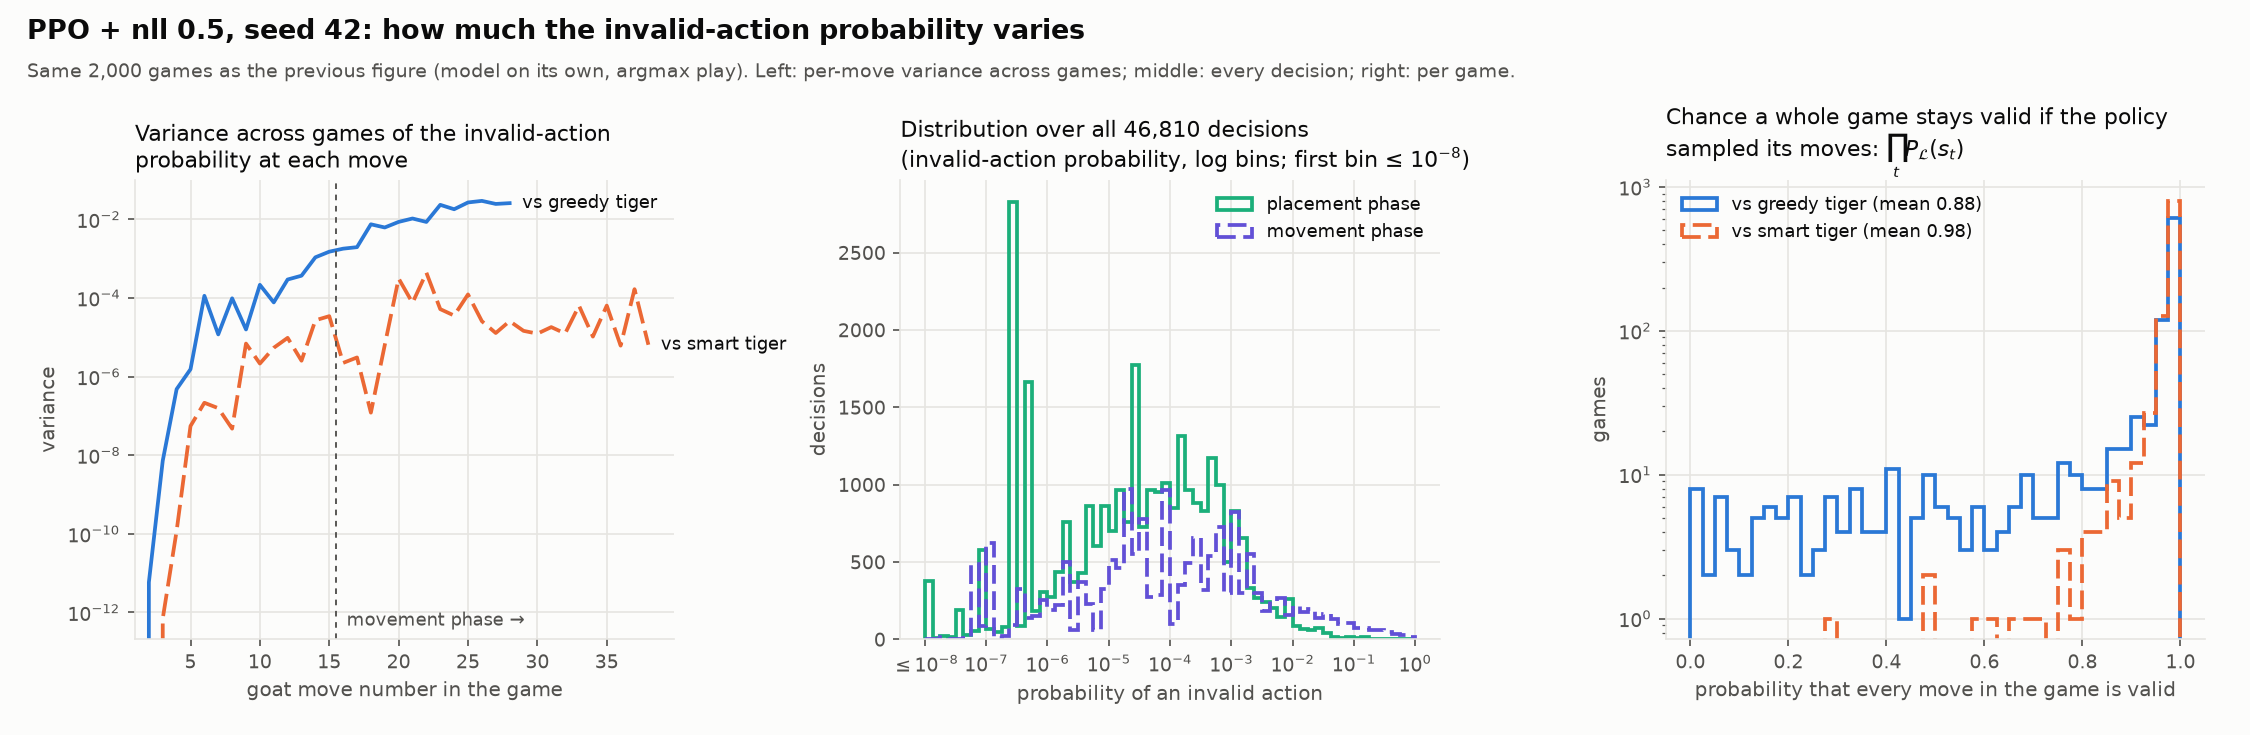
\includegraphics[width=0.98\linewidth]{figures/6_invalid_probability_variance.png}
\caption{Distribution and variance of the invalid-action probability for the same model.}\label{fig:variance}
\end{figure}

\section{Models against each other and against perfect play}\label{sec:comparisons}

Sections \ref{old:7}--\ref{old:9} compared models through win rates against the two scripted tigers. With the
game solved, three sharper questions can be asked. How do the models fare against each other? How do they
fare against a player that never errs? And, move by move, how often do they change the value of the
position? The experiment is \code{perfect\_play/compare\_models.py}; its results are in
\code{perfect\_play/tables/model\_comparison.json}.

\subsection{Setup}\label{sec:cmp-setup}

\textbf{Players.} Table~\ref{tab:players} lists them. Models play their deterministic masked move
(Section~\ref{old:3.2}), as in all earlier evaluations.

\begin{table}[H]
\centering\small
\caption{Players in the comparison.}\label{tab:players}
\begin{tabular}{@{}>{\raggedright\arraybackslash}p{0.22\linewidth}p{0.74\linewidth}@{}}
\toprule
Name & Player \\
\midrule
Perfect & reads the tables: fastest win, slowest loss. Among drawing moves it prefers positions not yet seen in the game, then the move after which the largest share of the opponent's replies lose (``trap-seeking'') \\
Perfect (plain) & reads the tables; picks uniformly among the moves of equal value and distance, with no preference among drawing moves \\
Random & uniform over legal moves \\
Greedy, Smart & the scripted tigers of Section~\ref{old:2.4} \\
NormalGoat, SmartGoat, RobustGoat & the shipped goat models (Section~\ref{old:6.2}; 100M, 100M and 60M steps) \\
PPO+nll & plain PPO with the legality loss, $c_{\text{legal}} = 0.5$, tanh, seed 42, 10M steps (Section~\ref{old:6.4}) \\
ReLU-Mask & Maskable PPO, ReLU, seed 42, 10M steps (Section~\ref{old:6.4}) \\
Tiger-N, Tiger-S, RobustTiger & the shipped tiger models, trained against NormalGoat, SmartGoat and RobustGoat \\
\bottomrule
\end{tabular}
\end{table}

\textbf{Games.} Every goat player meets every tiger player in 200 games from the opening, goats first, under
\code{TnGEnv}'s limits (200 plies; fourth repeat of a board with the goats to move). Game $i$ uses seed
$20{,}000 + i$ for all random choices. Two models always play the same game, so those pairings have one game.

\textbf{Judging moves.} Before and after each move the exact value of the position is read from the tables.
A move is a \textbf{blunder} if it lowers the value for the side that made it:
$\W{\to}\D$ (a forced win becomes a draw), $\W{\to}\Lo$, or $\D{\to}\Lo$ (a draw becomes a forced loss). All
other moves are value-preserving. A perfect player makes no blunders by construction; the tables confirm it
on its 382{,}163 decisions here.

\subsection{Results}

\begin{table}[H]
\centering\footnotesize
\caption{Round robin. Each cell is \emph{goat wins / tiger wins} in percent of 200 games; the rest are draws
by the turn limit or the repeat rule. $^\dagger$~Two deterministic models play one game: G, T or D is its
result.}\label{tab:roundrobin}
\begin{tabular}{@{}l cccccccc@{}}
\toprule
\tabin{generated/tab_roundrobin_head}
\midrule
\tabin{generated/tab_roundrobin}
\bottomrule
\end{tabular}
\end{table}

\begin{figure}[H]
\centering
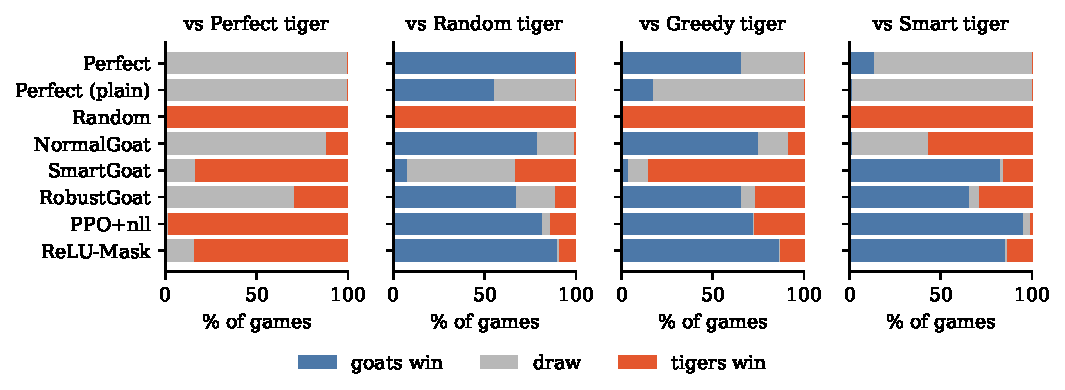
\includegraphics[width=\linewidth]{figures/outcomes_goat_players.pdf}
\caption{Outcomes of each goat player against four reference tigers (200 games each).}\label{fig:outcomes}
\end{figure}

\begin{table}[H]
\centering\footnotesize
\caption{Models against the perfect player, in percent of 200 games. ``Blunders'' is the mean number of
$\D{\to}\Lo$ moves per game; ``first'' is the mean ply of the first blunder in the games that have one.}\label{tab:vsperfect}
\begin{tabular}{@{}ll rrr r rr@{}}
\toprule
\multicolumn{8}{@{}l}{\textbf{Goat players against a perfect tiger}} \\
goats & perfect tiger & wins & draws & losses & plies & blunders & first \\
\midrule
\tabin{generated/tab_goats_vs_perfect}
\midrule
\multicolumn{8}{@{}l}{\textbf{Tiger players against a perfect goat}} \\
tigers & perfect goat & wins & draws & losses & plies & blunders & first \\
\midrule
\tabin{generated/tab_tigers_vs_perfect}
\bottomrule
\end{tabular}
\end{table}

\begin{table}[H]
\centering\footnotesize
\caption{Move quality of each player over all its round-robin games. ``Decisions in'' gives the share of the
player's decisions taken in positions that were won, drawn or lost for it. ``Win thrown'' is the share of
decisions in won positions that gave the win away; ``draw lost'' the share of decisions in drawn positions
that led to a forced loss. ``Converted'' counts the games in which the player held a forced win at some
point, and how many of them it won.}\label{tab:quality}
\begin{tabular}{@{}ll r rrr rr r l@{}}
\toprule
 & & & \multicolumn{3}{c}{decisions in (\%)} & \multicolumn{2}{c}{blunder rate (\%)} & blunders & \\
\cmidrule(lr){4-6}\cmidrule(lr){7-8}
 & player & decisions & won & drawn & lost & win thrown & draw lost & per 100 & converted \\
\midrule
\tabin{generated/tab_quality}
\bottomrule
\end{tabular}
\end{table}

\begin{figure}[H]
\centering
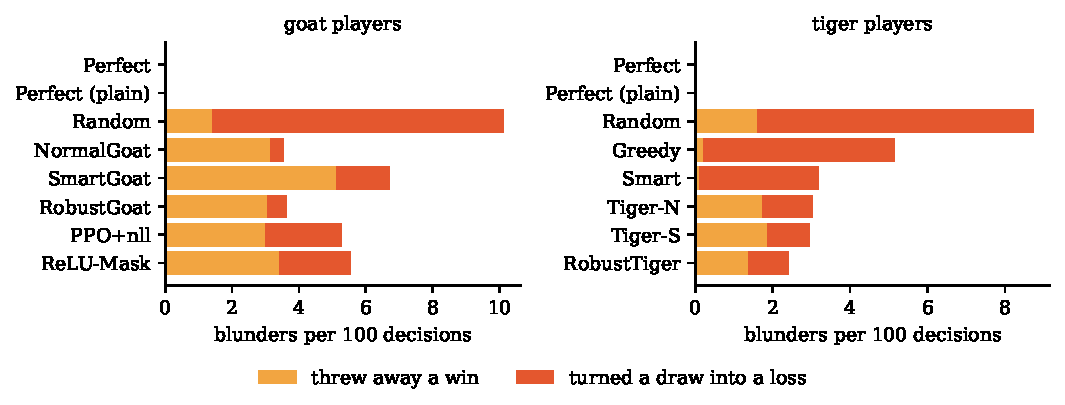
\includegraphics[width=\linewidth]{figures/blunders.pdf}
\caption{Blunders per 100 decisions, by kind, over all round-robin games of each player.}\label{fig:blunders}
\end{figure}

\subsection{Models against models}\label{sec:cmp-models}

Two deterministic models produce a single game, which says little. To get a distribution, the first four
plies are drawn uniformly from the moves that keep the game a draw; the models then play on. Those four
plies are not scored. Every game therefore starts from a different balanced position.

\begin{table}[H]
\centering\footnotesize
\caption{Goat models against tiger models from 200 balanced random openings, in percent. The last two
columns are blunders per 100 decisions of each side.}\label{tab:openings}
\begin{tabular}{@{}ll rrr r rr@{}}
\toprule
goats & tigers & goat wins & draws & tiger wins & plies & goat blunders & tiger blunders \\
\midrule
\tabin{generated/tab_openings}
\bottomrule
\end{tabular}
\end{table}

\subsection{The effect of the capture correction}\label{sec:cmp-fix}

The win rates of Section~\ref{old:9} were measured before the capture rule was corrected
(Section~\ref{sec:rulefix}); the round robin uses the corrected rule. To separate the two, the goat models
were replayed against the scripted tigers under both rules, 1{,}000 games each. Under the old rule a tiger
jumping from \code{d1} over \code{c1} to \code{b1} removes the goat on \code{b0} if there is one and otherwise
none.

\begin{table}[H]
\centering\footnotesize
\caption{Goat win rate under the old and the corrected capture rule (1{,}000 games per cell; standard error
at most 0.016). ``Study'' repeats the value of Sections \ref{old:9.1} and \ref{old:9.4}, measured in \code{TnGEnv}
before the correction. $\Delta$ is corrected minus old, in percentage points.}\label{tab:capturefix}
\begin{tabular}{@{}l rrrr rrrr@{}}
\toprule
 & \multicolumn{4}{c}{against Greedy} & \multicolumn{4}{c}{against Smart} \\
\cmidrule(lr){2-5}\cmidrule(l){6-9}
goats & study & old rule & corrected & $\Delta$ & study & old rule & corrected & $\Delta$ \\
\midrule
\tabin{generated/tab_capturefix}
\bottomrule
\end{tabular}
\end{table}

The ``old rule'' columns reproduce the study's values within sampling error, which confirms that the game
loop used here plays the same game as \code{TnGEnv} and that the difference in the other columns is the rule.

\subsection{Analysis}\label{sec:cmp-analysis}

\paragraph{1. Nobody beats the perfect player, and perfect against perfect is a draw.} All 800 games between
the two perfect players were drawn, 798 of them at the 200-ply limit and 2 by the repeat rule. In 5{,}600 games against other players a perfect player
never lost (Table~\ref{tab:roundrobin}, first two rows and columns). This is the solved value of the game seen
in play.

\paragraph{2. The goat models can all be beaten, some almost always.} Against the trap-seeking perfect tiger
the goats lose 11.5\% (NormalGoat), 29.5\% (RobustGoat), 83.5\% (SmartGoat), 84.0\% (ReLU-Mask) and 98.0\%
(PPO+nll) of their games (Table~\ref{tab:vsperfect}). A single $\D{\to}\Lo$ move decides each of these games: the
mean number of such blunders per game equals the loss rate, because the perfect tiger converts every one.
The first blunder comes late, on average between ply 43 and ply 91, well after the opening.

\paragraph{3. Strength against the training opponent and soundness are different things.} PPO+nll is the
strongest goat against the Smart tiger (96\% wins) and the easiest for a perfect tiger to beat (98\% losses).
NormalGoat wins only 2\% against Smart but holds a perfect tiger to a draw in 88.5\% of games. This is the
best-response effect of Section~\ref{sec:fp-br}: each model is tuned to the mistakes of its opponent and has
never been punished for its own. The longest-trained models (100M and 60M steps) are the hardest to exploit,
with SmartGoat the exception.

\paragraph{4. The tiger models fall into traps every time.} Against the trap-seeking perfect goat, all three
tiger models lose 200 games out of 200, in about 30 plies: they are immobilized as the placement phase ends.
The scripted Smart tiger survives 86.5\% of such games and even the Greedy tiger 34.5\%. Yet by average move
quality the tiger models are the \emph{best} non-perfect tigers, with 2.4--3.0 blunders per 100 decisions
against 3.2 for Smart (Table~\ref{tab:quality}). Against the plain perfect goat, which does not look for traps,
they draw 86--92\% of games. Average blunder rate measures typical play; exploitability measures the worst
case. A deterministic player with a few fixed weak spots can look good on the first and be lost on the second,
because a deterministic opponent that finds the weak spot finds it in every game.

\paragraph{5. A perfect player is not the best exploiter.} The plain perfect goat wins 17.5\% of its games
against Greedy and 1.5\% against Smart. NormalGoat wins 75\% against Greedy; PPO+nll wins 96\% against Smart.
Perfect play guarantees the value of the game, a draw, and nothing more: among moves that keep the draw it
has no reason to prefer the one the opponent is most likely to answer badly. Adding a one-ply preference
for traps raises the perfect goat to 65.5\% against Greedy, 13.5\% against Smart, 99.5\% against Random and 100\% against
the tiger models, still below the specialists against their own training opponent. The models earn their
wins by steering play into positions where that opponent errs: NormalGoat takes 46\% of its decisions in
positions that are already won for it.

\paragraph{6. Winning a won game is the hard part for some models.} Once a forced win is on the board, the
goat models convert it in 35\% (SmartGoat) to 90\% (ReLU-Mask) of games; the Random goat never does
(Table~\ref{tab:quality}). SmartGoat gives the win away in 30.7\% of its decisions in won positions, against
6.8--12.1\% for the other models. The tiger models give away 36--42\%, but for a tiger one wasted move in a
won position is often harmless, and they still convert all but one of the games in which they held a win.

\paragraph{7. Between models, the tigers come out ahead.} In the nine deterministic pairings of shipped models
the tigers win seven and draw two. From balanced random openings (Table~\ref{tab:openings}) the tigers win
between 19\% and 89\% of games and the goats at most 17.5\% (NormalGoat against RobustTiger). Blunder rates
are higher here than against scripted opponents, 5--14 per 100 decisions for the goats and 4--11 for the
tigers. A random opening and an unfamiliar opponent take both sides off the positions they were trained on.

\paragraph{8. The capture correction cost the models that leaned on the old rule.}
Table~\ref{tab:capturefix}: RobustGoat drops by 19 points against Greedy and 21 against Smart, and SmartGoat by
8 against Smart. Under the old rule a goat on \code{c1} could not be captured from \code{d1}, and these models
had learned to rely on it. NormalGoat and the two 10M-step models are unaffected (within one standard
error), although they too were trained under the old rule. All win rates in Section~\ref{old:9} should be
read with this in mind: they describe the game the models were trained on, not the corrected one.

\paragraph{9. Scale.} A uniformly random player makes 8.7 (tigers) to 10.1 (goats) blunders per 100
decisions. The trained models make 2.4--6.7. In drawn positions, where most decisions are made, the goat
models lose the draw in 0.8--3.3\% of decisions and the tiger models in 1.2--1.5\%, against 3.5\% for Smart
and 7.9\% for Greedy. The models have learned most of what keeps a position safe, and the remaining 1--3\% is
what a perfect opponent finds.

\paragraph{Limitations.}
\begin{itemize}
\item Each pairing has 200 games, so a percentage carries a standard error of up to 3.5 points.
\item Move quality in Table~\ref{tab:quality} pools a player's games against all opponents, which visit
  different positions. It ranks players loosely, not precisely.
\item Only games with the goats moving first were played. Models play deterministically.
\item The trap preference looks one ply ahead. A deeper search for the opponent's likely errors would
  exploit weak players more, at no risk.
\item One seed per training configuration, as in Section~\ref{old:9}.
\end{itemize}


\appendix
\part*{Appendices}
\addcontentsline{toc}{part}{Appendices}
\section{Reward functions and knobs}\label{app:rewards}
This appendix gives the full reward of each learner role. Part~II needs only that $r_t$ is a bounded function
of the transition; the details matter for reproducing a model.
\subsection{Goat-learner reward $r^{\text{goat}}_t$}\label{old:2.5}

\code{\_\allowbreak{}sparse\_\allowbreak{}reward\_\allowbreak{}goat}, \code{env\_\allowbreak{}tng.py:616}. Features (all computed in \code{\_\allowbreak{}step\_\allowbreak{}goat\_\allowbreak{}transition}):

{\footnotesize
\begin{longtable}{@{}>{\raggedright\arraybackslash}p{\dimexpr 0.113\linewidth-2\tabcolsep\relax}>{\raggedright\arraybackslash}p{\dimexpr 0.566\linewidth-2\tabcolsep\relax}>{\raggedright\arraybackslash}p{\dimexpr 0.264\linewidth-2\tabcolsep\relax}>{\raggedright\arraybackslash}p{\dimexpr 0.057\linewidth-2\tabcolsep\relax}@{}}
\toprule
\textbf{Symbol} & \textbf{Definition} & \textbf{Measured at} & \textbf{Code} \\
\midrule
\endhead
$M^+_t$ & $M(b^+_t)$, tiger mobility after the goat action; $M^+_{-1} = M(b_0)$ & before the reply & \code{:999} \\
$\Delta M_t$ & $M^+_{t-1} - M^+_t$ (positive = goats removed tiger options) & consecutive pre-reply boards & \code{:1011} \\
$U(b)$ & number of cells with $b_i \in \{0,1\}$ that no tiger can reach by walking through \textbf{empty} cells & — & \code{:1755} \\
$\Delta U_t$ & $U(b^+_t) - U(b^+_{t-1})$ & pre-reply boards & \code{:1015} \\
$\Sigma(b)$ & $\sum_{i<j} \text{dist}(x_i, x_j)$ over tiger squares $x$; graph distance ignoring pieces & — & \code{:1830} \\
$\Delta\Sigma_t$ & $\Sigma(b^+_{t-1}) - \Sigma(b^+_t)$ (positive = tigers pushed together) & pre-reply boards & \code{:1019} \\
$\ell_t$ & near-lock: $\ind[0 < M^+_t \leq 2]$ & $b^+_t$ & \code{:1005} \\
$Z^{\text{g}}_t$ & $\sum_{i \in K} \big(\knob{REWARD\_CENTER\_GOAT}\,\ind[b^+_{t,i}=1] + \knob{REWARD\_CENTER\_TIGER}\,\ind[b^+_{t,i}=2]\big)$, $K = \{0, 9, 10, 15, 16\}$ & $b^+_t$ & \code{:1022} \\
$k_t$ & goats captured by the reply: $c_{t+1} - c_t$ & after the reply & \code{:1080} \\
$h_t$ & earlier visits of the key $(b_{t+1}, c_{t+1}, \phi_{t+1})$ at post-reply checkpoints in this episode & after the reply & \code{:1107} \\
$\eta_t$ & shaping decay: $\knob{GOAT\_SHAPING\_DECAY\_BASE}^{\,n^{\text{mv}}_{t+1}}$ if $\phi_{t+1} = 1$, else 1 & after the step & \code{:679} \\
$\sigma_t$ & step cost: $\knob{REWARD\_STEP}$ if $\phi_t = 0$, else $\max\big(\knob{MOVE\_STEP\_BASE} + \knob{MOVE\_STEP\_SLOPE}\, n^{\text{mv}}_t,\ \knob{MOVE\_STEP\_MIN}\big)$ & before the action & \code{:949} \\
\bottomrule
\end{longtable}\addtocounter{table}{-1}
}

\textbf{Invalid actions and the goat win replace everything else:}

\[
r^{\text{goat}}_t = \begin{cases}
\knob{REWARD\_INVALID\_SOFT} & \text{invalid\_soft (illegal placement)} \\
\knob{REWARD\_INVALID\_HARD} & \text{invalid\_hard (illegal slide)} \\
\knob{REWARD\_GOAT\_WIN} - \knob{GOAT\_WIN\_TURN\_DECAY}\cdot \tau_{t+1} & \text{goat win} \\
\sum_k r^{(k)}_t & \text{otherwise}
\end{cases}
\]
Let $\chi_t$ flag a losing ending:
\[
\chi_t = \ind\big[\text{reason} \in \{\text{capture threshold},\ \text{max\_timeout},\ \text{repeat\_timeout}\}\big].
\] The decomposition matches the \code{info["reward\_\allowbreak{}*\_\allowbreak{}component"]} fields:

{\footnotesize
\begin{longtable}{@{}>{\raggedright\arraybackslash}p{\dimexpr 0.103\linewidth-2\tabcolsep\relax}>{\raggedright\arraybackslash}p{\dimexpr 0.278\linewidth-2\tabcolsep\relax}>{\raggedright\arraybackslash}p{\dimexpr 0.619\linewidth-2\tabcolsep\relax}@{}}
\toprule
\textbf{$k$} & \textbf{Component $r^{(k)}_t$} & \textbf{Formula} \\
\midrule
\endhead
step & \code{reward\_\allowbreak{}step\_\allowbreak{}component} & $\sigma_t$ \\
near-lock & \code{reward\_\allowbreak{}near\_\allowbreak{}lock\_\allowbreak{}component} & $(1-\chi_t)\ \knob{NEAR\_LOCK\_BONUS}\ \eta_t\ \ell_t$ \\
block & \code{reward\_\allowbreak{}block\_\allowbreak{}component} & $(1-\chi_t)\, B_t$, with $B_t$ below \\
bubble & \code{reward\_\allowbreak{}bubble\_\allowbreak{}component} & $(1-\chi_t)\ \knob{REWARD\_BUBBLE\_SPACE}\ \tanh(\Delta U_t)\ \eta_t\ \ind[\Delta U_t > 0]$ \\
cluster & \code{reward\_\allowbreak{}cluster\_\allowbreak{}component} & $(1-\chi_t)\ \knob{REWARD\_CLUSTER\_TIGERS}\ \tanh(\Delta\Sigma_t)\ \eta_t\ \ind[\Delta\Sigma_t > 0]$ \\
centre & \code{reward\_\allowbreak{}center\_\allowbreak{}component} & $(1-\chi_t)\ Z^{\text{g}}_t\ \ind[\phi_{t+1} = 0]$ \\
goat eaten & \code{reward\_\allowbreak{}goat\_\allowbreak{}eaten\_\allowbreak{}component} & $\knob{REWARD\_GOAT\_EATEN}\ k_t$ \\
repeat & \code{reward\_\allowbreak{}repeat\_\allowbreak{}component} & $(1-\chi_t)\ \knob{REWARD\_REPEAT\_STATE}\ h_t^2$ \\
terminal & \code{reward\_\allowbreak{}terminal\_\allowbreak{}component} & $\knob{REWARD\_TIGER\_WIN}\cdot S_t$, with $S_t$ below \\
(logged) & \code{reward\_\allowbreak{}decay\_\allowbreak{}mult} & $\eta_t$ (a multiplier, not added) \\
\bottomrule
\end{longtable}\addtocounter{table}{-1}
}

\[
B_t = \begin{cases} \lvert\knob{REWARD\_BLOCK\_TIGER}\rvert\ \tanh(\Delta M_t)\ \eta_t & \Delta M_t > 0 \\ \lvert\knob{REWARD\_BLOCK\_TIGER}\rvert\ \knob{MOBILITY\_BACKSLIDE\_SCALE}\ \Delta M_t & \Delta M_t < 0 \\ 0 & \Delta M_t = 0 \end{cases}
\]
\[
S_t = \begin{cases} 1 & \text{capture threshold} \\ \knob{MAX\_TIMEOUT\_SCALE} & \text{max\_timeout} \\ \knob{REPEAT\_STALL\_SCALE} & \text{repeat\_timeout} \\ 0 & \text{otherwise} \end{cases}
\]
Notes:

\begin{itemize}
\item Positive shaping is squashed by $\tanh$ and decayed by $\eta_t$. The mobility \emph{backslide} is linear in $\Delta M_t$ and not decayed. The step cost, centre term and capture penalty are never decayed.
\item $U$ counts every goat cell as unreachable, because the search never enters a goat square. Every placement on a reachable cell therefore raises $U$ by at least 1, so $r^{(\text{bubble})}$ fires on most placements.
\item The knob comment for $\knob{REWARD\_CLUSTER\_TIGERS}$ says ``spreading tigers apart'', but the code rewards a \emph{decrease} in $\Sigma$, i.e. tigers pushed together.
\item The centre score is measured on $b^+_t$ (before the reply), but gated by the post-reply phase $\phi_{t+1}$. The step that places the 15th goat therefore earns no centre term.
\item A \code{late} factor is computed and logged (\code{:1006}) but \textbf{not used} by the reward:
\[
\min\!\Big(\frac{\max(\tau_{t+1} - \knob{LATE\_GAME\_START\_TURN},\ 0)}{\knob{MAX\_TURNS} - \knob{LATE\_GAME\_START\_TURN}},\ 1\Big)
\]
\item The stall fires at $h_t = \knob{MAX\_REPEATS} - 1$; on that step the terminal term replaces the repeat penalty.
\item In the lose-a-turn variant, an invalid attempt on the final turn gets $\knob{REWARD\_STEP} + \knob{REWARD\_TIGER\_WIN}\cdot\knob{MAX\_TIMEOUT\_SCALE}$. Its \code{info} has no \code{step\_\allowbreak{}penalty} and no features, so the defaults apply.
\end{itemize}
\subsection{Tiger-learner reward $r^{\text{tiger}}_t$}\label{old:2.6}

\code{\_\allowbreak{}sparse\_\allowbreak{}reward\_\allowbreak{}tiger}, \code{env\_\allowbreak{}tng.py:790}. Features (from \code{\_\allowbreak{}step\_\allowbreak{}tiger\_\allowbreak{}transition}):

{\footnotesize
\begin{longtable}{@{}>{\raggedright\arraybackslash}p{\dimexpr 0.125\linewidth-2\tabcolsep\relax}>{\raggedright\arraybackslash}p{\dimexpr 0.750\linewidth-2\tabcolsep\relax}>{\raggedright\arraybackslash}p{\dimexpr 0.125\linewidth-2\tabcolsep\relax}@{}}
\toprule
\textbf{Symbol} & \textbf{Definition} & \textbf{Code} \\
\midrule
\endhead
$k_t$ & goats captured by the tiger's own move ($0$ or $1$) & \code{:1198} \\
$\Delta M^{\text{T}}_t$ & $M(b^+_t) - M(b^+_{t-1})$: mobility after this tiger move minus mobility after the previous tiger move ($M(b_0)$ at reset). The goat reply in between is included & \code{:1200–1203} \\
$Z^{\text{t}}_t$ & $\lvert\knob{REWARD\_CENTER\_GOAT}\rvert\ \big(\#\{i \in K: b^+_{t,i} = 2\} - \#\{i \in K: b^+_{t,i} = 1\}\big)$ & \code{:1205–1210} \\
\bottomrule
\end{longtable}\addtocounter{table}{-1}
}

\[
r^{\text{tiger}}_t = \begin{cases}
\knob{REWARD\_INVALID\_SOFT} & \text{invalid\_soft (malformed action)} \\
-\lvert\knob{REWARD\_INVALID\_HARD}\rvert & \text{invalid\_hard (illegal tiger move)} \\
r^{\text{play}}_t & \text{otherwise}
\end{cases}
\]
\begin{align*}
r^{\text{play}}_t ={}& \knob{REWARD\_STEP} + \knob{REWARD\_TIGER\_CAPTURE}\ k_t + \lvert\knob{REWARD\_BLOCK\_TIGER}\rvert\ \Delta M^{\text{T}}_t \\
&+ \ind[\phi_{t+1} = 0]\ Z^{\text{t}}_t + r^{\text{term}}_t
\end{align*}
{\small\[
r^{\text{term}}_t = \begin{cases}
+\knob{REWARD\_TIGER\_WIN\_BONUS} & \text{capture threshold or no goat moves} \\
-\knob{REWARD\_TIGER\_LOSS\_PENALTY} & \text{goat win} \\
-\knob{REWARD\_TIGER\_LOSS\_PENALTY}\cdot\knob{MAX\_TIMEOUT\_SCALE} & \text{max\_timeout} \\
0 & \text{otherwise}
\end{cases}
\]}
Notes:

\begin{itemize}
\item Unlike the goat reward:
\begin{itemize}
\item the shaping terms are kept on terminal steps;
\item mobility is linear (no $\tanh$, no decay);
\item there is no movement-phase step ramp, no repeat penalty, and no \code{reward\_\allowbreak{}*} component logging. Only the total is returned, and the component fields stay at their zero defaults.
\end{itemize}
\item The tiger centre term reuses $\lvert\knob{REWARD\_CENTER\_GOAT}\rvert$ for both signs; $\knob{REWARD\_CENTER\_TIGER}$ is ignored.
\item \code{invalid\_\allowbreak{}hard} returned $+\lvert\knob{REWARD\_INVALID\_HARD}\rvert$ before v1.1, rewarding illegal tiger moves. It is negative from v1.1 on (\code{env\_\allowbreak{}tng.py:822}).
\item In the lose-a-turn variant, an invalid attempt on the final turn gets the step cost minus the timeout penalty, $\knob{REWARD\_STEP} - \knob{REWARD\_TIGER\_LOSS\_PENALTY}\cdot\knob{MAX\_TIMEOUT\_SCALE}$.
\end{itemize}
\subsection{Reward and game knobs (\code{DEFAULT\_\allowbreak{}KNOBS}, \code{env\_\allowbreak{}tng.py:78})}\label{old:2.7}

Any knob can be overridden per run or phase with \code{reward\_\allowbreak{}overrides} / \code{REWARD\_\allowbreak{}OVERRIDES}. Fixed game constants: 23 squares, 15 goats to place, 6 captures to win, tigers start on $\{0, 3, 4\}$.

{\small
\begin{longtable}{@{}lll@{}}
\toprule
\textbf{Knob} & \textbf{Default} & \textbf{Used in} \\
\midrule
\endhead
$\knob{REWARD\_GOAT\_WIN}$ & 3.2 & goat win, before turn decay \\
$\knob{REWARD\_TIGER\_WIN}$ & −3.2 & goat terminal loss; scaled for timeouts \\
$\knob{REWARD\_TIGER\_CAPTURE}$ & 0.35 & tiger: per capture \\
$\knob{REWARD\_TIGER\_WIN\_BONUS}$ & 3.2 & tiger win \\
$\knob{REWARD\_TIGER\_LOSS\_PENALTY}$ & 3.2 & tiger loss and timeout (subtracted) \\
$\knob{REWARD\_STEP}$ & −0.001 & step cost: goat placement phase, every tiger step \\
$\knob{REWARD\_GOAT\_EATEN}$ & −0.35 & goat: per goat captured \\
$\knob{MAX\_TIMEOUT\_SCALE}$ & 1.5 & timeout multiplier (both roles) \\
$\knob{REPEAT\_STALL\_SCALE}$ & 1.25 & goat repeat-stall multiplier \\
$\knob{MAX\_TURNS}$ & 100 & turn limit (also the \code{max\_\allowbreak{}turns} argument) \\
$\knob{MOVE\_STEP\_BASE}$ & −0.01 & goat movement-phase step cost, intercept \\
$\knob{MOVE\_STEP\_SLOPE}$ & −0.01 & goat movement-phase step cost, per prior goat move \\
$\knob{MOVE\_STEP\_MIN}$ & −0.6 & goat movement-phase step cost, floor \\
$\knob{GOAT\_WIN\_TURN\_DECAY}$ & 0.01 & goat win reward lost per turn \\
$\knob{REWARD\_BLOCK\_TIGER}$ & 0.08 & mobility shaping magnitude (both roles) \\
$\knob{REWARD\_BUBBLE\_SPACE}$ & 0.02 & goat: unreachable-cell shaping \\
$\knob{REWARD\_CLUSTER\_TIGERS}$ & 0.02 & goat: tiger-spread shaping \\
$\knob{REWARD\_CENTER\_GOAT}$ & 0.03 & centre squares (goat; magnitude for tiger) \\
$\knob{REWARD\_CENTER\_TIGER}$ & −0.03 & goat's centre score, per tiger on $K$ \\
$\knob{NEAR\_LOCK\_BONUS}$ & 0.05 & goat near-lock bonus \\
$\knob{LATE\_GAME\_START\_TURN}$ & 40 & \code{late} factor only (unused by the reward) \\
$\knob{MOBILITY\_BACKSLIDE\_SCALE}$ & 0.5 & goat: penalty multiplier when $\Delta M_t < 0$ \\
$\knob{GOAT\_SHAPING\_DECAY\_BASE}$ & 0.95 & base of $\eta_t$ \\
$\knob{REWARD\_INVALID\_SOFT}$ & −0.05 & invalid\_soft \\
$\knob{REWARD\_INVALID\_HARD}$ & −1.0 & invalid\_hard (tiger uses $-\lvert\cdot\rvert$) \\
$\knob{REWARD\_REPEAT\_STATE}$ & −0.5 & goat repeat penalty, times $h_t^2$ \\
$\knob{MAX\_REPEATS}$ & 4 & repeat-stall threshold \\
$\knob{BASE\_TIGER\_CAPTURE\_BIAS}$ & 1.0 & greedy tiger: probability of preferring captures \\
\bottomrule
\end{longtable}\addtocounter{table}{-1}
}


\section{Verification tests}\label{old:8}

All tests run the notebook's own code (its cells executed in a headless IPython shell or through \code{nbclient}).

{\footnotesize
\begin{longtable}{@{}>{\raggedright\arraybackslash}p{\dimexpr 0.048\linewidth-2\tabcolsep\relax}>{\raggedright\arraybackslash}p{\dimexpr 0.476\linewidth-2\tabcolsep\relax}>{\raggedright\arraybackslash}p{\dimexpr 0.476\linewidth-2\tabcolsep\relax}@{}}
\toprule
\textbf{\#} & \textbf{Test} & \textbf{Result} \\
\midrule
\endhead
1 & Masked deterministic choice equals \code{MaskablePPO.predict(\ldots{}, action\_\allowbreak{}masks)} (2 shipped goats × 2 tigers × 10 games) & 1,981 / 1,981 decisions equal \\
2 & \S\ref{old:5.3} with clip, MSE and $c_{\text{legal}} = 0$ matches SB3 \code{PPO} (same seed, 256 steps, 3 epochs) & $\max\lvert\Delta\theta\rvert = 0$ \\
3 & Stored masks match their observations: for placement states, $\mathcal{L}(s) = \{5p : b_p = 0\}$ & 128 / 128 \\
4 & Every loss variant trains, saves and reloads as plain \code{PPO} with its \code{loss\_\allowbreak{}settings} & pass (KL penalty adapted $\beta$ to 0.25) \\
5 & The legality loss lowers \code{train/illegal\_\allowbreak{}prob} (20k steps, $c_{\text{legal}} = 0$ vs 0.5) & 0.673 → 0.369 \\
6 & A tiger learner's illegal move is penalized (v1.1 fix) & $r = -1.00$, reason \code{invalid\_\allowbreak{}hard} \\
7 & Control center v1.1 vs v1.2 with tanh, both algorithms, 16,384 steps & $\max\lvert\Delta\theta\rvert = 0$ \\
8 & End-to-end notebook runs & 13 configurations pass. Three deliberate misconfigurations stop with a clear error: an unknown \code{ALGORITHM}, a run-level setting placed inside a phase, and resuming with several seeds \\
\bottomrule
\end{longtable}\addtocounter{table}{-1}
}

Test 8 covered:

\begin{itemize}
\item every feature switch and preset
\item both algorithms and all three policy losses
\item curriculum phases with model-goat mixing
\item resuming
\item several seeds per run, with masked and plain PPO in one \code{TRAINING\_\allowbreak{}RUNS}
\item both illegal-move modes
\item \code{ENV\_\allowbreak{}SOURCE = "repo"}
\item a fresh clone in a Colab-like empty folder
\end{itemize}

\section{The longest-win games}\label{app:games}
Each game runs from the opening to the record position by a shortest route and then follows perfect play to
the end (Section~\ref{sec:longest}). The moves before the record position are only a way to reach it, not good
play. Squares are numbered 0--22 (Figure~\ref{fig:board}); \code{@15} places a goat on square 15, \code{3-2} slides
a piece, and \code{10x0} is a capture landing on square 0. The text can be pasted into the visualizer
(\code{tngviz}, Ctrl+V) or loaded with \code{tngviz/run.sh -{}-game FILE}. Text copied from this PDF works too: line breaks are ignored.
\paragraph{Goats first: the goats' longest forced win (213 plies from ply 10).} File \code{perfect\_play/games/goats\_first\_goats\_win\_213.txt}.
\begin{gamelisting}
start: tigers=0,3,4 goats= captured=0 mover=goat\par
first: goat\par
moves: 1. @22 3-2 2. @18 2-8 3. @15 4-5 4. @6 0-2 5. @0 2-1 6. @3 5-4 7. @2 4-10 8. @19 1-7 9. @21 8-9 10. @20 10-16 11. @14 9-10 12. @4 7-13 13. @5 13-7 14. @11 7-8 15. @9 8-7 16. 2-8 7-1 17. 6-12 1-2 18. 22-17 2-1 19. 5-6 1-2 20. 21-22 2-1 21. 11-5 1-2 22. 17-11 2-1 23. 20-21 1-2 24. 22-17 2-1 25. 0-2 10x0 26. 15-20 1-7 27. 14-13 7-1 28. 19-14 1-7 29. 20-15 7-1 30. 21-22 16-10 31. 5-4 0-5 32. 4-0 5-4 33. 15-20 1-7 34. 14-19 7-1 35. 20-21 1-7 36. 17-16 4-5 37. 18-17 5-4 38. 19-20 7-1 39. 8-7 10x8 40. 11-10 8-9 41. 12-11 9-15 42. 6-12 15-9 43. 20-19 9-15 44. 21-20 15-9 45. 19-14 9-15 46. 14-8 15-9 47. 22-21 4-5 48. 10-4 5-6 49. 12-18 6-12 50. 16-10 12-6 51. 8-14 6-12 52. 14-15 12-6 53. 15-16 6-5 54. 18-12 5-6 55. 17-18 6-5 56. 16-17 5-6 57. 21-16 6-5 58. 12-6 9-8 59. 18-12 8-9 60. 16-15 9-8 61. 15-9 8-14 62. 10-16 14-15 63. 12-18 15-14 64. 20-15 14-19 65. 6-12 19-20 66. 11-10 5-11 67. 17-22 11-17 68. 4-5 20-21 69. 12-11 21-20 70. 0-4 20-21 71. 9-8 21-20 72. 10-9 20-19 73. 11-10 17-11 74. 5-6 11-17 75. 16-21 17-16 76. 15-20 16-17 77. 9-15 17-16 78. 15-14 16-17 79. 4-0 17-11 80. 10-16 11-17 81. 16-15 17-11 82. 18-17 11-5 83. 15-16 5-11 84. 6-12 11-5 85. 12-11 5-4 86. 17-18 4-5 87. 22-17 5-4 88. 18-12 4-5 89. 14-15 5-6 90. 17-18 6-5 91. 11-10 5-11 92. 8-9 11-5 93. 12-6 5-11 94. 6-5 19-14 95. 20-19 11-17 96. 5-4 14-8 97. 21-22 8-14 98. 9-8 17-11 99. 10-9 11-12 100. 4-10 12-6 101. 10-11 6-12 102. 9-10 12-6 103. 22-17 6-5 104. 10-4 5-6 105. 0-5 6-12 106. 4-10 12-6 107. 5-4 6-12 108. 4-0 12-6 109. 18-12 6x18 110. 0-5 18-12 111. 5-6 12-18 112. 11-12\par
result: Goats win (the tigers have no legal move) after 223 plies\par
\end{gamelisting}

\paragraph{Tigers first: the goats' longest forced win (214 plies from ply 14).} File \code{perfect\_play/games/tigers\_first\_goats\_win\_214.txt}.
\begin{gamelisting}
start: tigers=0,3,4 goats= captured=0 mover=tiger\par
first: tiger\par
moves: 1. 3-2 @22 2. 2-8 @21 3. 8-14 @20 4. 4-5 @19 5. 5-6 @18 6. 0-2 @16 7. 2-1 @10 8. 14-15 @4 9. 6-5 @3 10. 15-9 @0 11. 1-2 @14 12. 2-8 @2 13. 5-11 @15 14. 11-5 @6 15. 8-7 @8 16. 7-13 18-12 17. 9x11 8-9 18. 11-10 2-8 19. 13-7 16-17 20. 10-16 17-18 21. 7-1 8-2 22. 1-7 9-10 23. 7-13 2-8 24. 5-11 10-9 25. 13-7 0-2 26. 7-1 4-0 27. 11-5 22-17 28. 1-7 21-22 29. 5-4 12-11 30. 16-10 11-5 31. 7-13 20-21 32. 10-11 18-12 33. 11-10 17-11 34. 13-7 14-13 35. 10-16 19-14 36. 16-10 15-16 37. 7-1 11-17 38. 1-7 5-11 39. 7-1 14-15 40. 1-7 15-20 41. 7-1 8-7 42. 10x8 11-10 43. 8-9 12-11 44. 9-15 6-12 45. 15-9 20-19 46. 9-15 21-20 47. 15-9 19-14 48. 9-15 14-8 49. 15-9 22-21 50. 4-5 10-4 51. 5-6 12-18 52. 6-12 16-10 53. 12-6 8-14 54. 6-12 14-15 55. 12-6 15-16 56. 6-5 18-12 57. 5-6 17-18 58. 6-5 16-17 59. 5-6 21-16 60. 6-5 12-6 61. 9-8 18-12 62. 8-9 16-15 63. 9-8 15-9 64. 8-14 10-16 65. 14-15 12-18 66. 15-14 20-15 67. 14-19 6-12 68. 19-20 11-10 69. 5-11 17-22 70. 11-17 4-5 71. 20-21 12-11 72. 21-20 0-4 73. 20-21 9-8 74. 21-20 10-9 75. 20-19 11-10 76. 17-11 5-6 77. 11-17 16-21 78. 17-16 15-20 79. 16-17 9-15 80. 17-16 15-14 81. 16-17 4-0 82. 17-11 10-16 83. 11-17 16-15 84. 17-11 18-17 85. 11-5 15-16 86. 5-11 6-12 87. 11-5 12-11 88. 5-4 17-18 89. 4-5 22-17 90. 5-4 18-12 91. 4-5 14-15 92. 5-6 17-18 93. 6-5 11-10 94. 5-11 8-9 95. 11-5 12-6 96. 5-11 6-5 97. 19-14 20-19 98. 11-17 5-4 99. 14-8 21-22 100. 8-14 9-8 101. 17-11 10-9 102. 11-12 4-10 103. 12-6 10-11 104. 6-12 9-10 105. 12-6 22-17 106. 6-5 10-4 107. 5-6 0-5 108. 6-12 4-10 109. 12-6 5-4 110. 6-12 4-0 111. 12-6 18-12 112. 6x18 0-5 113. 18-12 5-6 114. 12-18 11-12\par
result: Goats win (the tigers have no legal move) after 228 plies\par
\end{gamelisting}

\paragraph{Goats first: longest win inside the 200-ply limit (191 plies from ply 6).} File \code{perfect\_play/games/goats\_first\_goats\_win\_within\_200\_plies\_191.txt}.
\begin{gamelisting}
start: tigers=0,3,4 goats= captured=0 mover=goat\par
first: goat\par
moves: 1. @17 3-9 2. @2 9-8 3. @1 0-5 4. @0 4-10 5. @3 5-11 6. @22 10-16 7. @18 11-10 8. @4 8-14 9. @7 10-9 10. @8 14-15 11. @19 15-20 12. @21 20-15 13. @20 16-10 14. @16 10-11 15. @10 11-12 16. 17-11 15x17 17. 4-5 17-16 18. 3-4 9-3 19. 22-17 16-15 20. 21-16 15-9 21. 16-15 12-6 22. 8-14 6-12 23. 2-8 12-6 24. 17-22 3-2 25. 22-21 2-3 26. 11-12 9x11 27. 8-9 11-17 28. 7-8 17-16 29. 1-7 16-10 30. 21-22 10-11 31. 20-21 11-10 32. 19-20 10-11 33. 21-16 11-10 34. 22-21 3-2 35. 9-3 10-9 36. 16-17 2-1 37. 14-13 1-2 38. 15-14 9-15 39. 21-16 15-9 40. 16-15 9-10 41. 17-22 10-11 42. 7-1 11-17 43. 13-7 17-11 44. 15-9 11-17 45. 20-15 17-11 46. 22-21 11-10 47. 15-16 10-11 48. 16-10 11-17 49. 9-15 17-16 50. 7-13 16-17 51. 21-16 17-22 52. 1-7 22-21 53. 8-9 2-8 54. 14-19 8-14 55. 3-2 21-22 56. 7-8 22-17 57. 10-11 17-22 58. 0-3 22-17 59. 9-10 17-22 60. 8-9 14-8 61. 2-1 8-14 62. 15-20 14-15 63. 16-21 15-14 64. 10-16 14-15 65. 16-17 15-14 66. 3-0 14-8 67. 9-10 8-14 68. 10-16 14-8 69. 13-14 8-2 70. 16-15 2-8 71. 1-7 8-2 72. 7-8 2-3 73. 14-13 3-9 74. 13-7 9-3 75. 19-14 3-9 76. 14-13 9-3 77. 8-9 3-2 78. 17-16 2-8 79. 11-10 8-2 80. 7-1 2-8 81. 1-2 22-17 82. 21-22 8-14 83. 2-3 14-8 84. 20-19 8-14 85. 10-11 14-8 86. 9-10 8-9 87. 19-20 9-8 88. 13-7 8-2 89. 7-1 2-8 90. 3-9 8-2 91. 20-19 2-8 92. 1-2 8-7 93. 2-8 7-1 94. 9-3 1-2 95. 19-14 2-1 96. 0-2 1-7 97. 10-9 7-1 98. 14-13 1-7 99. 2-1\par
result: Goats win (the tigers have no legal move) after 197 plies\par
\end{gamelisting}

\paragraph{Tigers first: longest win inside the 200-ply limit (193 plies from ply 7).} File \code{perfect\_play/games/tigers\_first\_goats\_win\_within\_200\_plies\_193.txt}.
\begin{gamelisting}
start: tigers=0,3,4 goats= captured=0 mover=tiger\par
first: tiger\par
moves: 1. 4-5 @19 2. 3-2 @4 3. 2-1 @3 4. 1-7 @9 5. 0x10 @8 6. 7-13 @0 7. 5-4 @2 8. 13-14 @18 9. 10-11 @21 10. 14-15 @22 11. 11-10 @12 12. 10-11 @17 13. 11-10 @16 14. 15-14 @15 15. 14-13 @14 16. 4-5 12-6 17. 5-4 18-12 18. 4-5 19-20 19. 5-4 17-11 20. 4-5 16-17 21. 5-4 0-5 22. 13-7 15-16 23. 7-13 20-15 24. 13-7 14-13 25. 7-1 5-0 26. 1-7 15-20 27. 7-1 8-7 28. 10x8 11-10 29. 8-9 12-11 30. 9-15 6-12 31. 15-9 20-19 32. 9-15 21-20 33. 15-9 19-14 34. 9-15 14-8 35. 15-9 22-21 36. 4-5 10-4 37. 5-6 12-18 38. 6-12 16-10 39. 12-6 8-14 40. 6-12 14-15 41. 12-6 15-16 42. 6-5 18-12 43. 5-6 17-18 44. 6-5 16-17 45. 5-6 21-16 46. 6-5 12-6 47. 9-8 18-12 48. 8-9 16-15 49. 9-8 15-9 50. 8-14 10-16 51. 14-15 12-18 52. 15-14 20-15 53. 14-19 6-12 54. 19-20 11-10 55. 5-11 17-22 56. 11-17 4-5 57. 20-21 12-11 58. 21-20 0-4 59. 20-21 9-8 60. 21-20 10-9 61. 20-19 11-10 62. 17-11 5-6 63. 11-17 16-21 64. 17-16 15-20 65. 16-17 9-15 66. 17-16 15-14 67. 16-17 4-0 68. 17-11 10-16 69. 11-17 16-15 70. 17-11 18-17 71. 11-5 15-16 72. 5-11 6-12 73. 11-5 12-11 74. 5-4 17-18 75. 4-5 22-17 76. 5-4 18-12 77. 4-5 14-15 78. 5-6 17-18 79. 6-5 11-10 80. 5-11 8-9 81. 11-5 12-6 82. 5-11 6-5 83. 19-14 20-19 84. 11-17 5-4 85. 14-8 21-22 86. 8-14 9-8 87. 17-11 10-9 88. 11-12 4-10 89. 12-6 10-11 90. 6-12 9-10 91. 12-6 22-17 92. 6-5 10-4 93. 5-6 0-5 94. 6-12 4-10 95. 12-6 5-4 96. 6-12 4-0 97. 12-6 18-12 98. 6x18 0-5 99. 18-12 5-6 100. 12-18 11-12\par
result: Goats win (the tigers have no legal move) after 200 plies\par
\end{gamelisting}

\paragraph{Goats first: the tigers' longest forced win (67 plies from ply 19).} File \code{perfect\_play/games/goats\_first\_tigers\_win\_67.txt}.
\begin{gamelisting}
start: tigers=0,3,4 goats= captured=0 mover=goat\par
first: goat\par
moves: 1. @2 3x1 2. @7 1x13 3. @18 0-5 4. @3 4x2 5. @12 2-0 6. @11 0-2 7. @10 2-0 8. @8 0-2 9. @7 2-1 10. @6 5x17 11. @15 13-14 12. @16 1x13 13. @2 13-7 14. @9 7-1 15. @3 17-11 16. 15-20 14-15 17. 16-21 11-5 18. 10-4 5-0 19. 4-10 15-16 20. 10-11 16-17 21. 6-5 17-22 22. 12-6 1-7 23. 6-12 7-13 24. 12-6 13-14 25. 6-12 14-15 26. 18-17 0-4 27. 5-6 15-14 28. 12-18 14-13 29. 18-12 13-7 30. 12-18 7-1 31. 18-12 4-5 32. 8-14 1-7 33. 14-8 5-0 34. 6-5 7-13 35. 5-6 13-14 36. 6-5 14-15 37. 5-6 15-16 38. 12-18 16-10 39. 18-12 0-4 40. 17-18 22-17 41. 11-5 4-0 42. 5-4 10-16 43. 2-1 0x10\par
result: Tigers win (6th goat captured) after 86 plies\par
\end{gamelisting}

\paragraph{Tigers first: the tigers' longest forced win (67 plies from ply 20).} File \code{perfect\_play/games/tigers\_first\_tigers\_win\_67.txt}.
\begin{gamelisting}
start: tigers=0,3,4 goats= captured=0 mover=tiger\par
first: tiger\par
moves: 1. 4-5 @2 2. 3x1 @7 3. 1x13 @2 4. 0x8 @18 5. 8-2 @12 6. 2-0 @11 7. 0-2 @10 8. 2-0 @8 9. 0-2 @7 10. 2-1 @6 11. 5x17 @15 12. 13-14 @16 13. 1x13 @2 14. 13-7 @9 15. 7-1 @3 16. 17-11 15-20 17. 14-15 16-21 18. 11-5 10-4 19. 5-0 4-10 20. 15-16 10-11 21. 16-17 6-5 22. 17-22 12-6 23. 1-7 6-12 24. 7-13 12-6 25. 13-14 6-12 26. 14-15 18-17 27. 0-4 5-6 28. 15-14 12-18 29. 14-13 18-12 30. 13-7 12-18 31. 7-1 18-12 32. 4-5 8-14 33. 1-7 14-8 34. 5-0 6-5 35. 7-13 5-6 36. 13-14 6-5 37. 14-15 5-6 38. 15-16 12-18 39. 16-10 18-12 40. 0-4 17-18 41. 22-17 11-5 42. 4-0 5-4 43. 10-16 2-1 44. 0x10\par
result: Tigers win (6th goat captured) after 87 plies\par
\end{gamelisting}


\section{Reproducing the numbers}\label{app:repro}

{\small
\begin{longtable}{@{}>{\raggedright\arraybackslash}p{0.52\linewidth}>{\raggedright\arraybackslash}p{0.44\linewidth}@{}}
\toprule
\textbf{Command (from the repository root)} & \textbf{Produces} \\
\midrule
\endhead
\code{python perfect\_play/prove\_rules.py} & rule and index equivalence with \code{TnGEnv} (Section~\ref{sec:dp-proof}); about 11 minutes \\
\code{python perfect\_play/solve.py} & movement tables and placement values; needs CuPy and a CUDA GPU \\
\code{python perfect\_play/solve\_placement\_dtm.py -{}-delete-u2} & placement ply counts \\
\code{python perfect\_play/check\_all.py} & the independent check of every position; about 3 minutes on 16 threads \\
\code{python perfect\_play/reachable.py} & reachable positions, longest forced wins and their games (Section~\ref{sec:longest}); about 1 minute \\
\code{python perfect\_play/compare\_models.py} & the comparison of Section~\ref{sec:comparisons}; needs torch and sb3-contrib, and the study models in \code{artifacts/legality\_study/}; about 1 minute \\
\code{python docs/mathematical\_architecture/make\_tables.py} & the generated tables and figures of this document \\
\code{pdflatex TnG\_Mathematical\_Architecture.tex} (twice, in \code{docs/mathematical\_architecture/}) & this PDF \\
\bottomrule
\end{longtable}\addtocounter{table}{-1}
}

The tables (21 GB) are not in the repository; the first three commands rebuild them in about a minute of GPU
time. The legality study of Section~\ref{old:9} is reproduced with \code{TnG\_Notebook.ipynb} and the run
configurations of Section~\ref{old:6.4}.

\end{document}
